\documentclass[lettersize,journal]{IEEEtran}
\usepackage{amsmath,amsfonts}
\DeclareMathOperator*{\argmax}{arg\,max}
\DeclareMathOperator*{\argmin}{arg\,min}
\usepackage{algorithm}
\usepackage{algpseudocode}
\usepackage{array}
% \usepackage[caption=false,font=normalsize,labelfont=sf,textfont=sf]{subfig}
\usepackage{textcomp}
\usepackage{stfloats}
\usepackage{url}
\usepackage{verbatim}
\usepackage{graphicx}
\usepackage{pgfplots}
\usepackage{svg}
\usepackage{cite}
\usepackage{kotex}
\usepackage{booktabs} % For better looking tables
\usepackage{caption} % For customising the captions
\usepackage{subcaption}
\usepackage{siunitx} % For alignment of numbers on decimal point
\usepackage{xcolor}
\hyphenation{op-tical net-works semi-conduc-tor IEEE-Xplore}
% updated with editorial comments 8/9/2021


% MACROS
\newcommand\ie{\textit{i.e.}}
\newcommand\eg{\textit{e.g.}}

\begin{document}

\title{Overcoming the Diffraction Limit: Self-Supervised Image Restoration using Terahertz Self-Aligned Hyperspectral Images}

\author{Woon-Ha Yeo, Seung-Hwan Jung, Inhee Maeng, Youngbin Ji, Seung Jae Oh*\thanks{* Corresponding author.}, and Han-Cheol Ryu*
        % <-this % stops a space
\thanks{This paper was produced by the IEEE Publication Technology Group. They are in Piscataway, NJ.}% <-this % stops a space
\thanks{Manuscript received April 19, 2023; revised August 16, 2023.}}

\markboth{Journal of \LaTeX\ Class Files,~Vol.~14, No.~8, August~2023}%
{Shell \MakeLowercase{\textit{et al.}}: A Sample Article Using IEEEtran.cls for IEEE Journals}

\IEEEpubid{0000--0000/00\$00.00~\copyright~2023 IEEE}
% Remember, if you use this you must call \IEEEpubidadjcol in the second
% column for its text to clear the IEEEpubid mark.

\maketitle

\begin{abstract}
This study proposes a novel self-supervised deep learning image restoration method to overcome the diffraction limit of terahertz (THz) imaging using a terahertz time-domain spectroscopy (THz-TDS) system. Our proposed method employs self-supervised learning using self-aligned hyperspectral (SAHS) data obtained through the THz-TDS system, without additional training datasets, thereby overcoming the diffraction limit of THz waves and enhancing image quality. The key to this learning method is that it can learn from the frequency characteristics of THz SAHS images without the need for artificial image degradation typically used in conventional image restoration learning. This paper presents a framework for self-supervised learning based on THz SAHS images, which includes one-to-one frequency mapping, recurrent learning, and zero-shot super-resolution. Experimental results demonstrate that the proposed method significantly improves the clarity of THz images by overcoming the diffraction limit in low-frequency regions and effectively reduces noise in high-frequency regions. These results are expected to enhance the image quality of various THz imaging systems by overcoming the THz wave’s diffraction limit and generating high-resolution images.
\end{abstract}

\begin{IEEEkeywords}
Deep learning, self-supervised learning, terahertz self-aligned hyperspectral images, terahertz time-domain spectroscopy, image restoration
\end{IEEEkeywords}

\section{Introduction}
Terahertz (THz) waves, situated in the electromagnetic spectrum between microwaves and infrared, span a frequency range of approximately 0.1 THz to 10 THz. They are utilized in various fields due to their unique properties. For instance, because THz waves can penetrate most non-metallic materials, they are beneficial in applications such as security scanning and non-destructive testing. Additionally, THz waves can capture information regarding the rotational and vibrational states of molecules, thus enabling their use in the detection and analysis of chemical substances; as well as the imaging of biological tissues.

Imaging across various electromagnetic wave bands, including X-rays and visible light, has revolutionized our daily lives. In medical diagnostics, X-ray imaging is crucial  for detecting conditions such as cancer and dental diseases, owing to its high penetration depth through various materials. Visible-light imaging has not only transformed the manner by which we record life but has also contributed to the development of artificial intelligence (AI) applications in surveillance security and surface-defect inspection. However, both of these imaging techniques have unresolved issues. Ionizing X-ray imaging can harm biological entities, thus severely limiting its application. Non-ionizing and non-destructive visible light imaging cannot probe the interiors of most optically opaque objects because of the highly absorptive and scattering behavior of light in the visible band.

THz imaging can be used to address these issues. THz imaging, which creates images by measuring the intensity or phase of THz waves, is non-ionizing and non-destructive and has garnered significant attention for its ability to classify materials as well as detect and inspect objects. Because THz radiation can partially penetrate various optically opaque materials, hidden information regarding the material is transmitted along with the wave, thus enabling the visualization of the interior without damaging the exterior~\cite{thz_imaging1,thz_imaging2,thz_imaging3,thz_imaging4}.

Over the recent decades, terahertz time-domain spectroscopy (THz-TDS) has become one of the most prominent forms of THz imaging; it enables non-invasive evaluations owing to its unique ability to extract the geometric and multifunctional information of objects. Because of its distinctive material interaction information in multi-dimensional domains such as space, time, frequency, and phase, THz-TDS imaging has been applied in various emerging areas, including drug detection~\cite{kawase2003nondest}, industrial inspection, cultural-heritage examination~\cite{fukunaga2016thz}, advanced-material investigation~\cite{spies2020terahertz}, and cancer detection~\cite{bowman2018pulsed}.

\begin{figure*}[htbp]
    \centering
    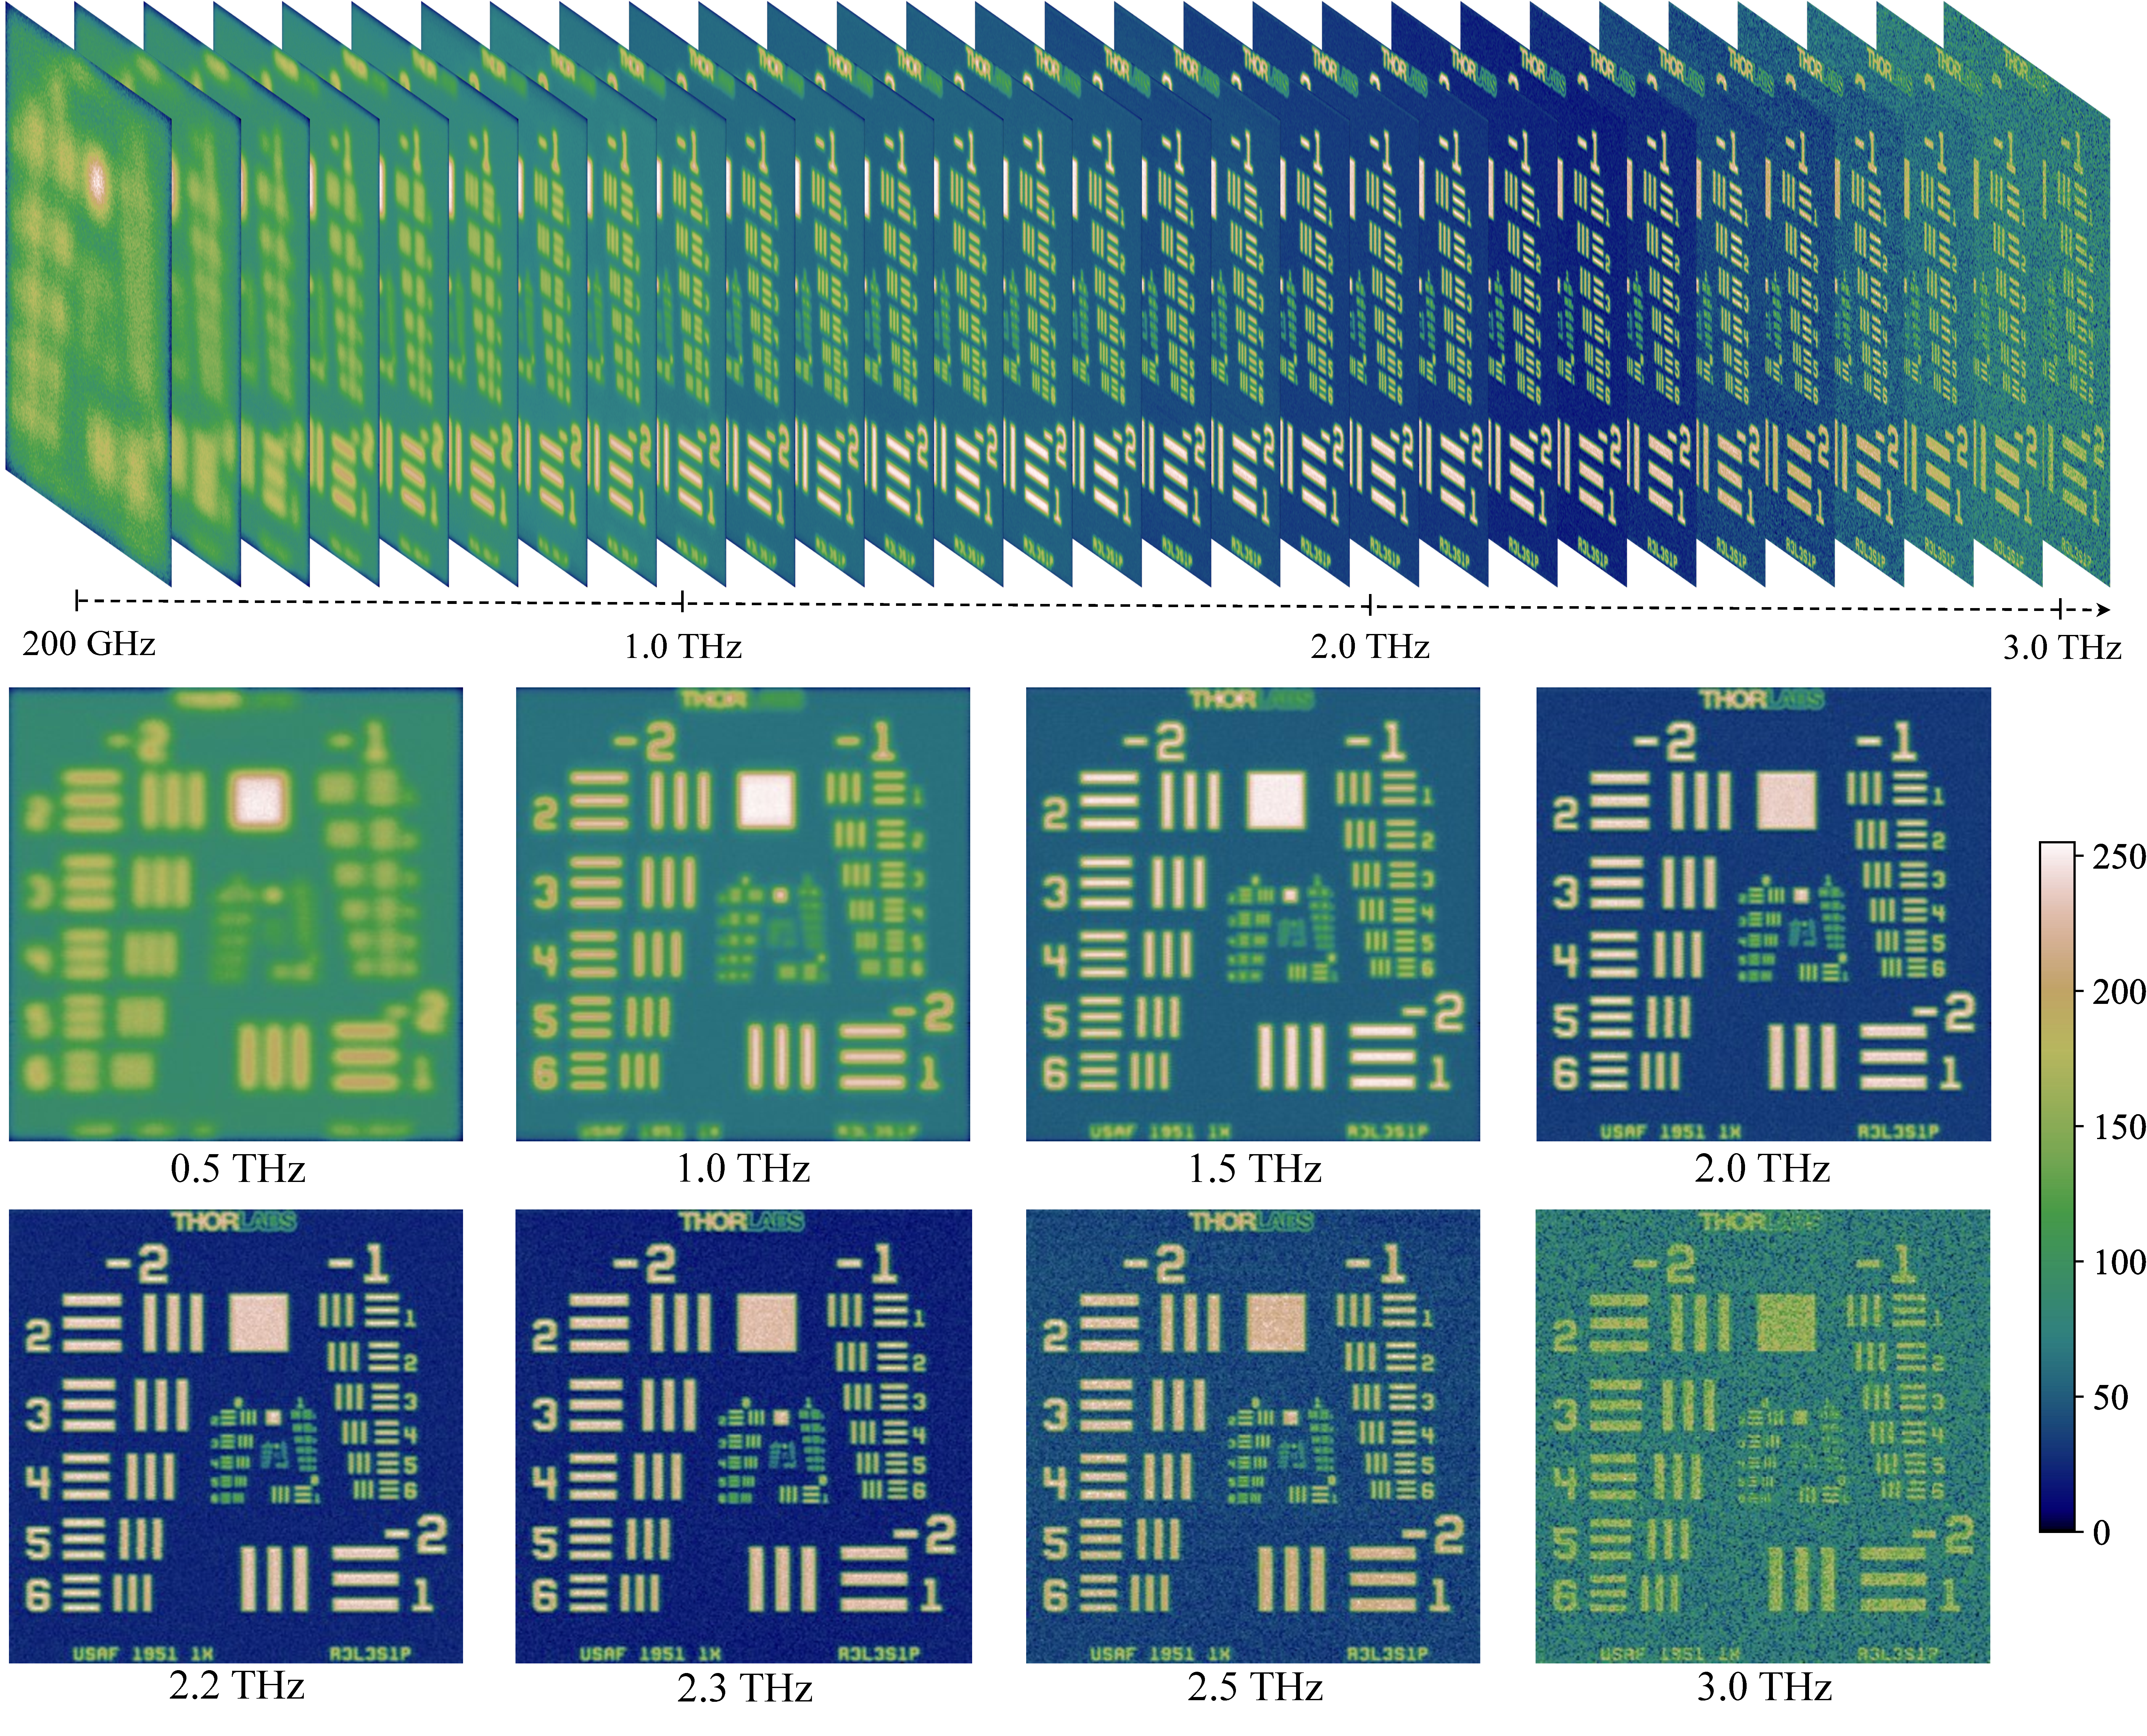
\includegraphics[width=0.85\textwidth]{fig/Ryu-fig1.pdf}
    \caption{THz SAHS image of the positive USAF 1951 resolution test target.}
    \label{fig:hyperspectral}
\end{figure*}

\IEEEpubidadjcol % 글자 겹치는거 방지용 
However, THz imaging is typically associated with image quality degradation owing to its strong water-absorption characteristics and low noise tolerance, thus resulting in undesirable blurring and distortion. Additionally, THz images obtained using THz-TDS system exhibit distinctly different characteristics depending on the frequency. Fig.~\ref{fig:hyperspectral} shows a THz self-aligned hyperspectral (SAHS) image obtained using the THz-TDS system of the positive United States Air Force (USAF) 1951 resolution test target (Thorlabs R3L3S1P). It shows frequency-specific images ranging from 200 GHz to 3 THz, in increments of 0.1 THz. Since the pixel values at the same location in SAHS images are acquired from the same TDS data, images of all frequencies within the SAHS image are automatically aligned without additional post-processing. All the THz images used in this study are based on the color map shown in Fig.~\ref{fig:hyperspectral}. Images in the lower-frequency band appear visually blurred but less noisy owing to the diffraction limit, whereas those in the higher frequencies offer better spatial resolution but increased noise owing to a lower signal-to-noise ratio (SNR).

Fig.~\ref{fig:iqa} shows the variations in the image sharpness, noise level, and contrast with frequency. The x-axis represents frequency, the left y-axis indicates the sharpness and noise level~\cite{chen2015noiselevel}, and the right y-axis represents the contrast. The image contrast increases gradually with frequency and reaches a maximum at 2.2 THz before decreasing. The sharpness increases continually with frequency, whereas the noise level decreases up to 1.0 THz and then increase as the frequency increase. The detailed descriptions of each image quality assessment metric are provided in Appendix~\ref{subsec:iqa}.

\begin{figure}[htbp]
    \centering
    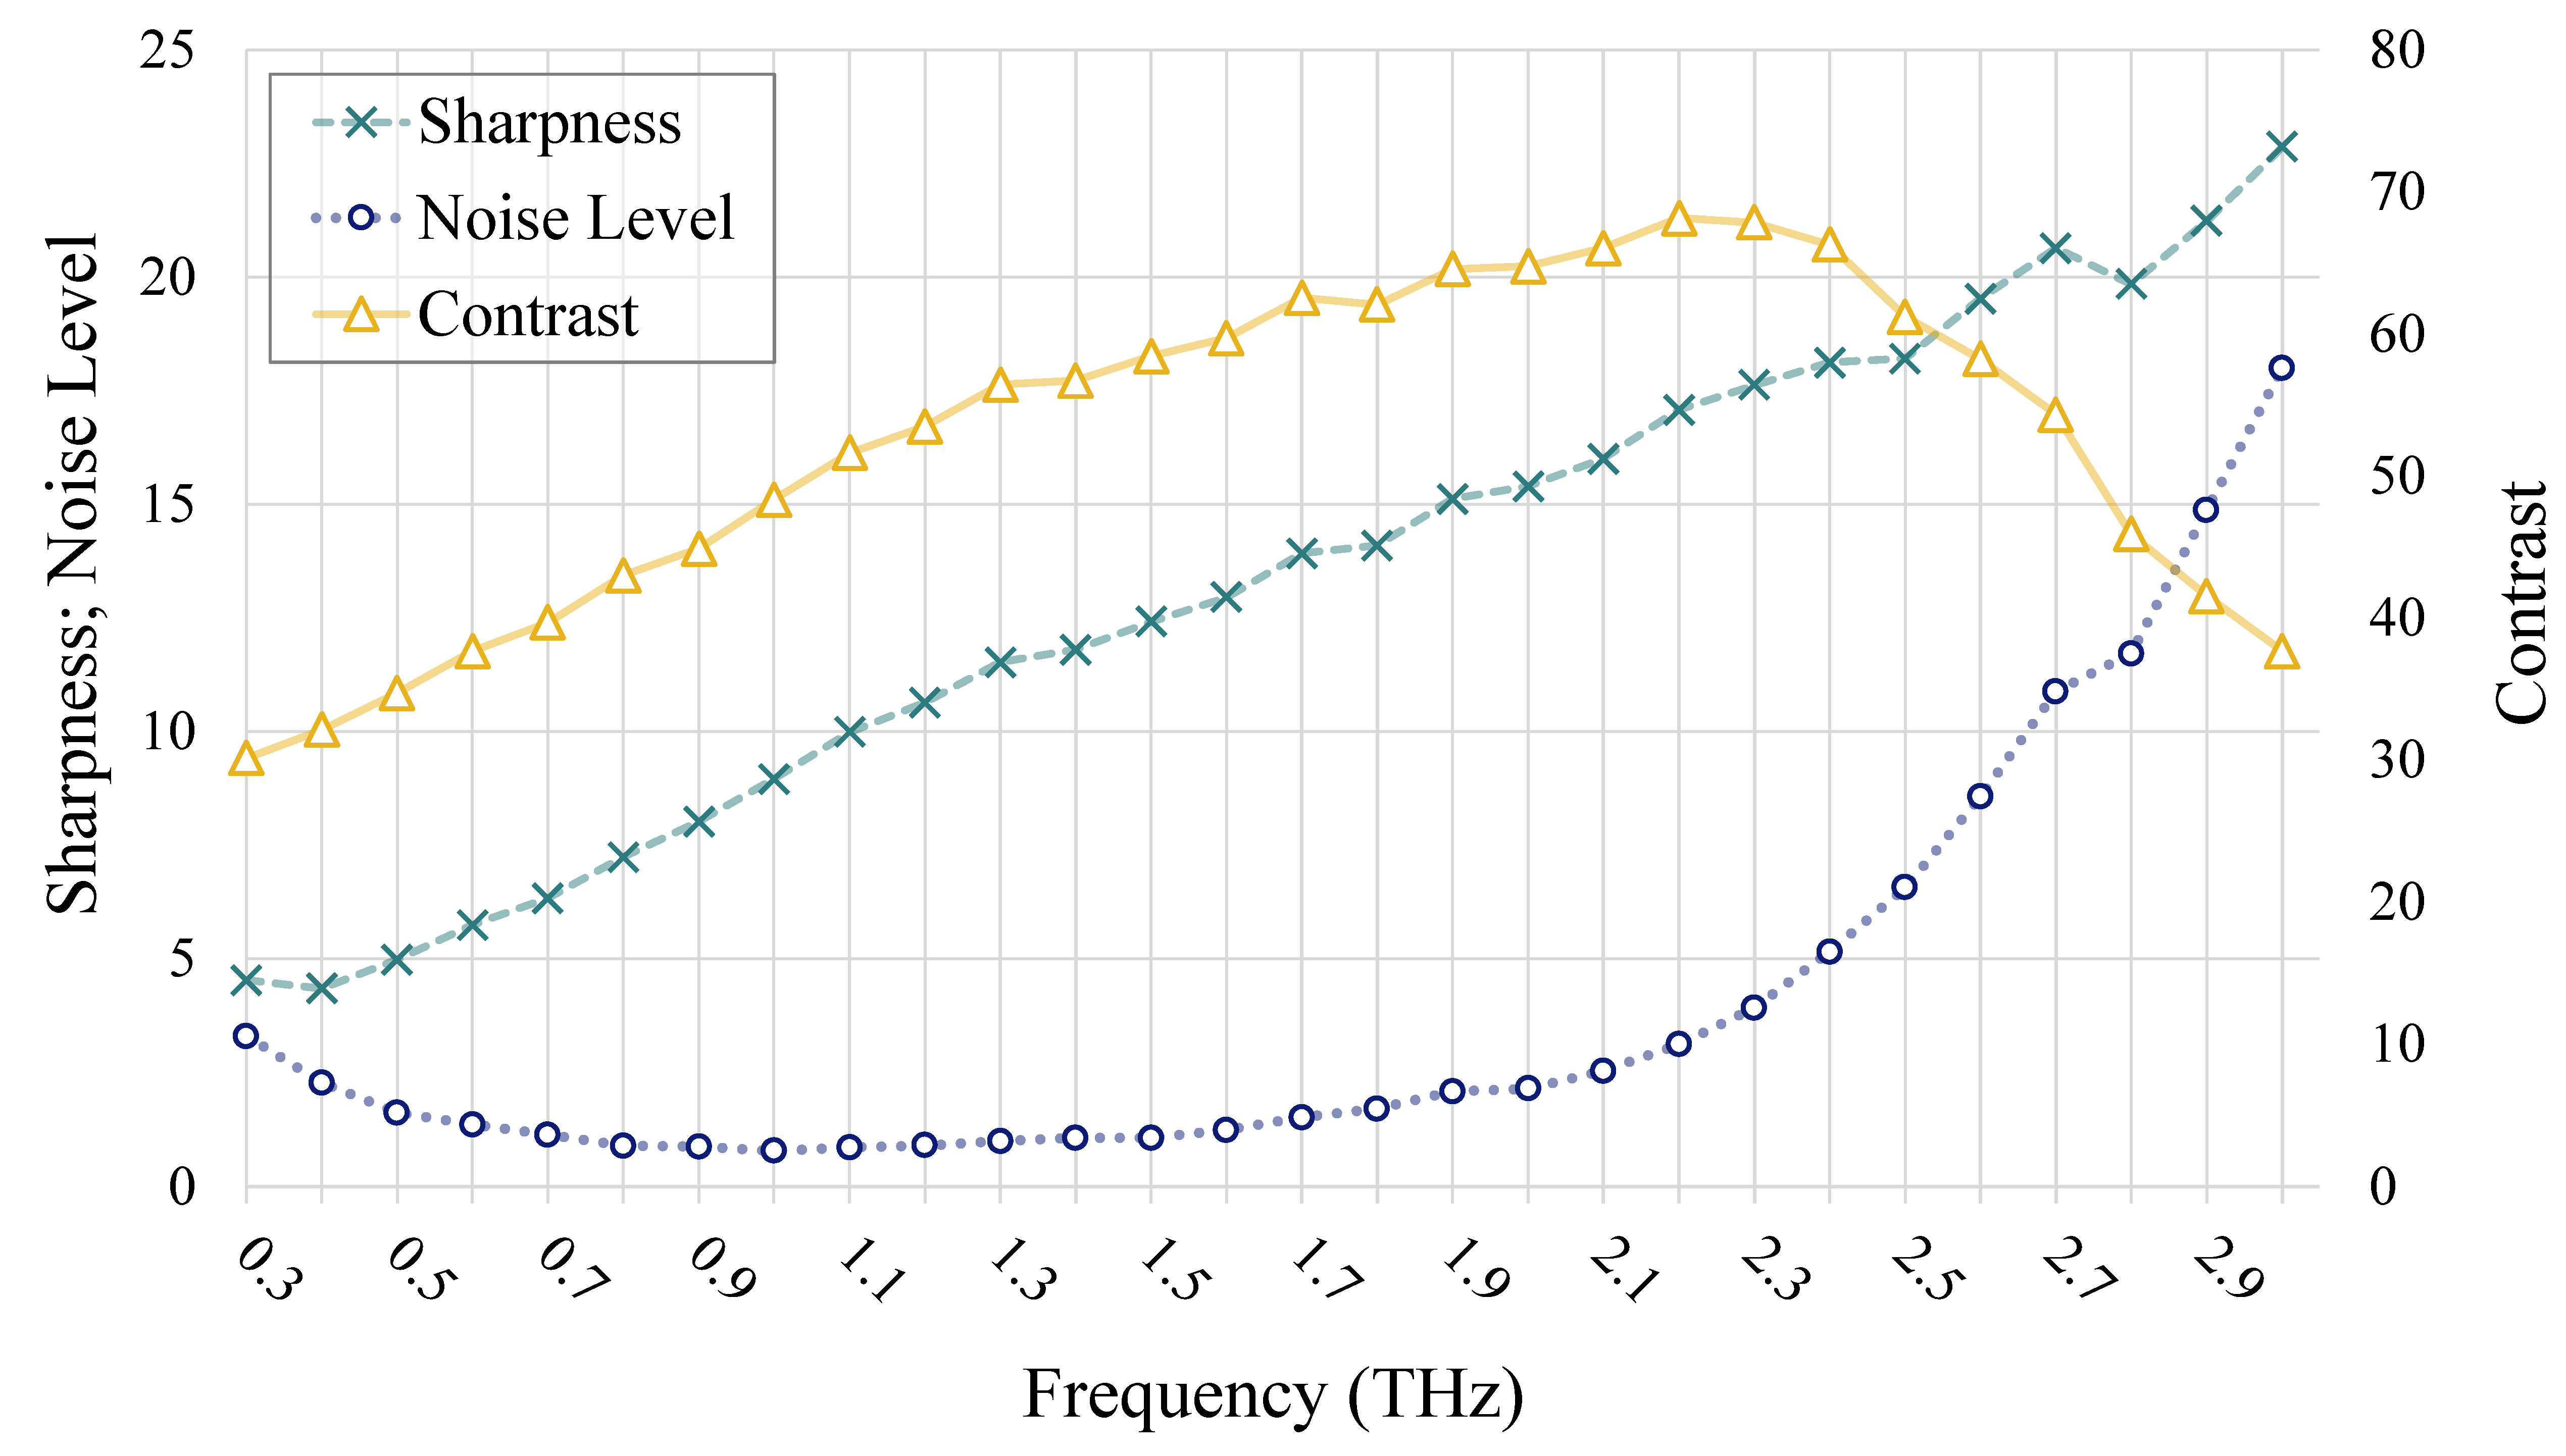
\includegraphics[width=\columnwidth]{fig/Ryu-fig2.pdf}
    \caption{Image quality assessment of the original THz SAHS images.}
    \label{fig:iqa}
\end{figure}

Conventional supervised-learning methods can be used to remove blurs in low-frequency images and noise in high-frequency images to achieve clearer images. However, applying supervised learning to THz images is challenging due to the difficulty in obtaining clean target images that directly correspond to these THz images. Hence, this study proposes a method for enhancing the quality of THz images through self-supervised learning using THz SAHS images obtained from a THz-TDS imaging system. Additionally, owing to the wavelength size and technical limitations of the imaging system, the typical image pixel resolution in THz imaging is extremely low. To overcome this, we apply image super-resolution (SR) based on self-supervised learning.

The primary objective of this study is to enhance the quality of an image obtained from a single measurement by utilizing the image. To achieve this, we propose a framework that includes a series of self-supervised image restoration methods using THz SAHS images. By performing self-supervised learning, the THz image data can be trained  without clean image targets, thereby enabling the learning of complex patterns necessary for THz image restoration.

Specifically, we train a deep learning model to learn the mapping between THz frequency bands, either from low to high frequency or vice versa. The model, which is trained to map from low to high frequency, enables blurry low-frequency images to emulate the characteristics of sharp high-frequency images. Additionally, this trained model can be applied to previously unseen images without requiring further training to render them as clear as high-frequency images. This implies that the model can overcome the diffraction limit of THz low-frequency images to yield results similar to those of high-frequency images without noise. This process of learning mapping between two frequency images can be repeated to further improve the image quality. Furthermore, using a model trained for high-to-low-frequency mapping enables noise reduction in noisy high-frequency images, although this may slightly degrade the image sharpness. Finally, we apply the zero-shot image super-resolution (ZSSR) technique, which can increase the resolution of an image by itself, to obtain visually enhanced images from a single THz SAHS image.


% 5. Main contributions %
The main contributions of this study are summarized as follows:
\begin{itemize}
\item We propose a framework that includes a series of processes to restore a single THz SAHS image obtained from a single measurement using a THz-TDS system.
\item We propose a self-supervised image restoration method based on one-to-one (O2O) mapping between frequencies, which utilizes the characteristics of a single THz SAHS image obtained via THz-TDS.
\item Our method can create images resembling high-frequency images by overcoming the diffraction limit of  low-frequency THz images and it can also reduce noise in high-frequency THz images with low SNRs.
\item The model trained using our proposed method is not limited to a specific imaging system and can be applied to all electromagnetic wave-based images.
\end{itemize}
\subsection{Deep Image Restoration}
\label{sec:dir}
In general optical image restoration, deep learning-based methods, particularly those based on convolutional neural networks (CNNs), have demonstrated significantly better performance than conventional model-based image restoration methods~\cite{gu2012fast, timofte2013anchored, timofte2015a+, michaeli2013nonparametric, he2010single}. These methods typically learn mapping from low-quality to high-quality images using large-scale paired datasets. Notable CNN-based image restoration networks include the SRCNN~\cite{dongSRCNN2014}, a CNN architecture for image SR, and the DnCNN~\cite{zhangDnCNN2017} for image denoising, along with others~\cite{kim2016accurate, wang2018esrgan, zhang2021plug, zhang2020residual, peng2019dilated, chen2022simple, fu2021model}. Recently, Transformer-based image restoration methods~\cite{liangSwinIRImageRestoration2021, wangUformerGeneralUShaped2022, chenActivatingMorePixels2023} have emerged, following the success of Transformers~\cite{vaswani2017attention} in computer vision. However, these learning methods typically require large-scale training datasets.


\subsection{THz Image Restoration}
Conventional algorithm-based methods for THz image restoration primarily rely on deconvolution procedures~\cite{li2010continuous, ding2010high, xu2014high, wongComputationalImageEnhancement2018, ningResolutionEnhancementTerahertz2019}. These methods depend on the accurate estimation of the beam point spread function (PSF) of THz imaging systems. Owing to the success of deep learning in image restoration, researchers have begun to apply it to THz image restoration has also begun. In particular, researchers have applied the leading methods of deep image restoration to optical images, as introduced in Section~\ref{sec:dir}. Dong et al.~\cite{liTerahertzImageSuperresolution2017a} trained the SRCNN~\cite{dongSRCNN2014} model on 91 natural images. Henceforth, various studies pertaining to for THz image restoration have been conducted ~\cite{leiTerahertzTimedomainSuperresolution2021,wongTrainingAutoencoderbasedOptimizers2019,marinaljubenovicJointDeblurringDenoising2020,hanTerahertzImageRestoration2020,wangTerahertzImageSuperresolution2021,longTerahertzImageSuperresolution2019,zhangRestorationIntegratedCircuit2021,zhangTerahertzImageRestoration2022,luMathematicalDegradationModel2021a,ruanEfficientSubpixelConvolutional2022,maoImageFusionBased2020,suDataDrivenBasedTerahertzImage2023,liAdaptiveTerahertzImage2020,wangComplexZeroshotSuperresolution2022,ljubenovicCNNbasedDeblurringTerahertz2020,yangSuperresolutionReconstructionTerahertz2022,ljubenovicBeamShapeEffectsNoise2022}. 

Lei et al.~\cite{leiTerahertzTimedomainSuperresolution2021} investigated the potential of a graph neural network (GNN) by training it on 8 THz images and testing it on one image.
Wong et al.~\cite{wongTrainingAutoencoderbasedOptimizers2019} investigated the image restoration of frequency modulation continuous wave (FMCW) three-dimensional (3D) images using AutoEncoders, thus providing a novel approach in THz imaging for 3D image restoration.
Marinal et al.~\cite{marinaljubenovicJointDeblurringDenoising2020} investigated a non-deep learning-based approach for THz image restoration that does not require the estimation of the PSF of a beam.
Han et al.~\cite{hanTerahertzImageRestoration2020} were the first to employ ZSSR technique in THz image restoration, which entails  learning directly from an image without requiring additional external data.
Wang et al.~\cite{wangTerahertzImageSuperresolution2021} used a complex CNN (CCNN) to enhance the quality of THz images.
Long et al.~\cite{longTerahertzImageSuperresolution2019} presented a method using a network based on residual connections, which marked a significant advancement in THz image restoration.
Zhang et al.~\cite{zhangRestorationIntegratedCircuit2021} developed a wavelet denoising technique for integrated circuits that reduced noise in THz images.
Zhang et al.~\cite{zhangTerahertzImageRestoration2022} provided a benchmark dataset; however, it was synthetically generated using a PSF and may not be optimized for all THz imaging systems.
Lu et al.~\cite{luMathematicalDegradationModel2021a} developed a mathematical degradation model for restoring THz images.
Ruan et al.~\cite{ruanEfficientSubpixelConvolutional2022} improved the restoration quality of THz images using an efficient sub-pixel convolutional network (ESPCN)~\cite{shi2016real}.
Su et al.~\cite{suDataDrivenBasedTerahertzImage2023} investigated the synthesis of THz images using a data-driven approach.
Li et al.~\cite{liAdaptiveTerahertzImage2020} performed THz image restoration using an adaptive network.
Wang et al.~\cite{wangComplexZeroshotSuperresolution2022} proposed a complex ZSSR (CZSSR) technique that utilizes complex domain data.
Ljubenovic et al.~\cite{ljubenovicCNNbasedDeblurringTerahertz2020} applied CNN-based deblurring to aTHz-TDS system to improve the quality of THz images.
Yang et al.~\cite{yangSuperresolutionReconstructionTerahertz2022} implemented SR to THz images using a residual channel attention network (RCAN)~\cite{zhang2018image} structure.

Recent investigations into THz image restoration have progressed significantly through the application of various deep learning techniques. However, a key challenge is the absence of effective training datasets. Most studies have adopted widely used optical image datasets~\cite{agustsson2017ntire, timofte2017ntire} to emulate the characteristics of actual THz images. In this process, synthetic THz images are created by estimating the PSF of the THz imaging system and applying an isotropic Gaussian blur to the optical images.
However, this approach requires the optimization of the PSF for each THz imaging system. Hence, researchers adopted a random degradation approach that applies various forms of blur. However, the PSF in actual THz imaging systems is not precisely isotropic and varies from system to system. Moreover, THz images have characteristics different from those of conventional optical images. Therefore, models trained on artificially generated data using optical images exhibit performance limitations when directly applied to various THz images.

To address these challenges, we propose a self-supervised learning method using hyperspectral images obtained from a THz-TDS system. This approach does not rely on artificially degrading the image quality for training; instead, it learns the frequency characteristics of the acquired hyperspectral images, thereby overcoming the limitations of conventional training methods. This closely mirrors the actual characteristics of THz imaging systems, thereby enhancing the efficiency and accuracy of THz image restoration.






\section{Self-supervised image restoration via THz SAHS images}
\subsection{Data Acquisition}
THz SAHS images were acquired using a THz-TDS reflection setup, as shown in Fig.~\ref{fig:system}. THz pulses were generated using femtosecond and photoconductive antennas. The femtosecond laser featured a central wavelength of 1.5 μm and a pulse width of 80 fs. A fiber-coupled antenna (TERA15-TX-FC, Menlo Systems) was used as the photoconductive antenna to generate THz pulses, and another fiber-coupled dipole antenna (TERA15-RX-FC, Menlo Systems) was used to detect THz signals. To acquire THz signals rapidly, we employed an ultrafast scanner with a frequency and time width of 20 Hz and 30ps, respectively.

The THz signal was amplified using a low-noise current preamplifier (SRS570, Stanford Research) and subsequently digitized using a data-acquisition board. The generated THz pulses were guided through polymethylpentene (TPX) lenses and plate mirrors. The TPX lens focused the THz signal onto the sample stage, and the signal reflected from the sample was guided to the detector through a silicon beam splitter andanother TPX lens. All components except for the sample were placed within a dry air chamber to avoid signal distortion due to water vapor absorption. To obtain a two-dimensional image, the sample was shifted along the x- and y-axes to form a THz image with a spatial resolution of 282$\times$282 pixels, totaling 79,524 pixels. The time-domain signals obtained at each pixel were transformed into the frequency domain via the fast Fourier transform (FFT) to acquire broadband THz-wave characteristics.

\begin{figure}[htbp]
    \centering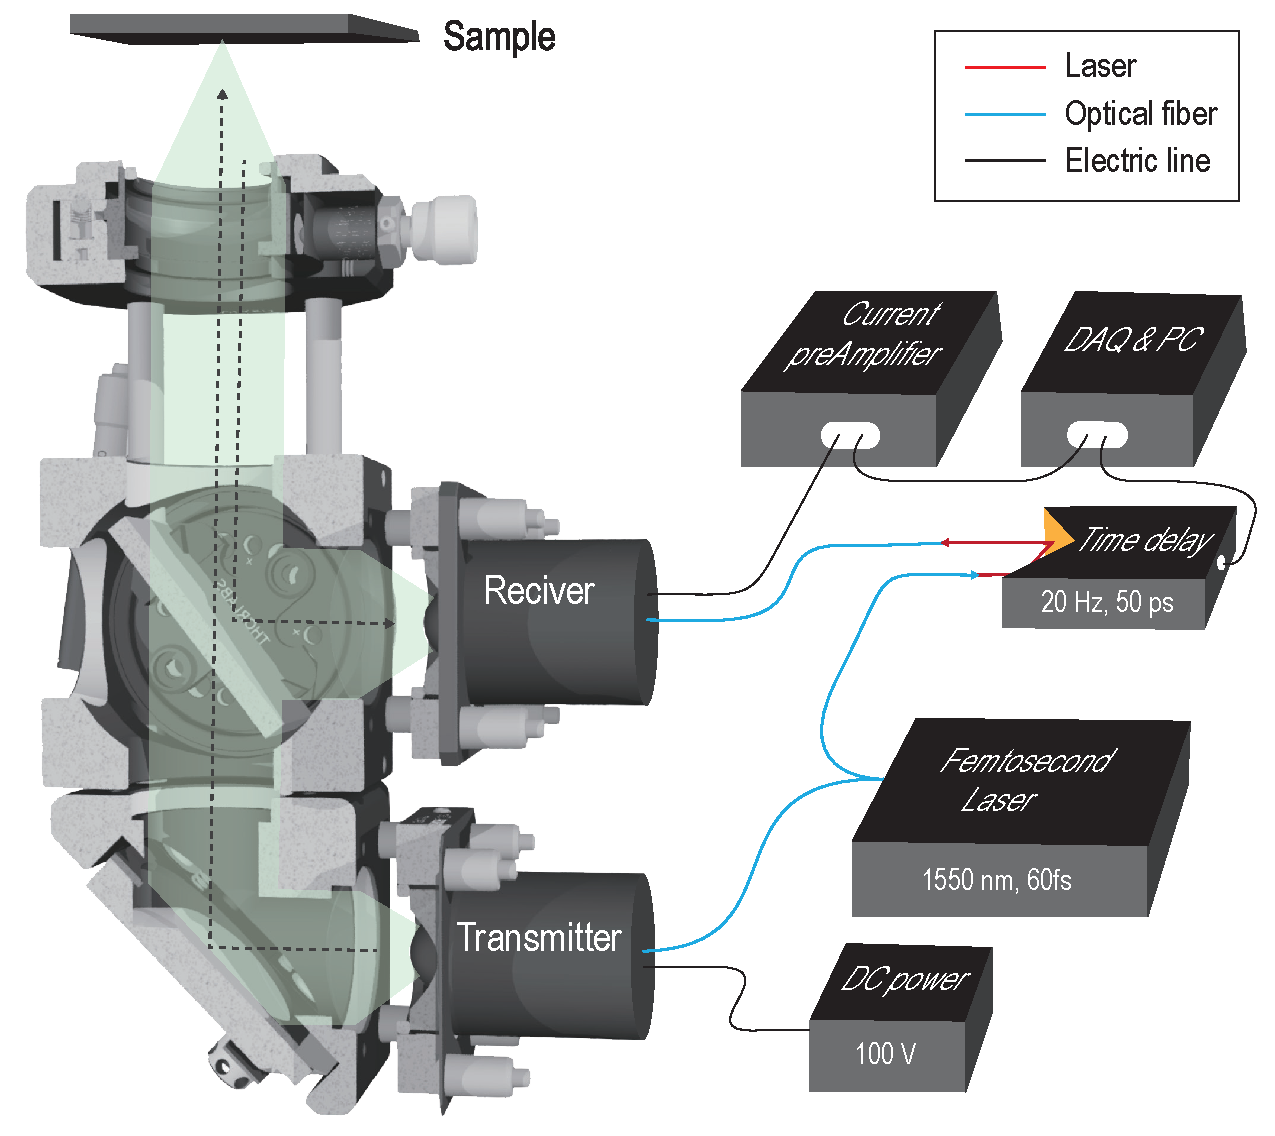
\includegraphics[width=\columnwidth]{fig/Ryu-fig3.pdf}
    \caption{Configuration of a THz-TDS imaging system.}
    \label{fig:system}
\end{figure}


\subsection{Diffraction Limit in Optics} % Preliminary

The diffraction limit refers to the theoretical minimum spatial resolution of optical and electromagnetic imaging systems. Equation~\ref{eq:resolution} expresses the diffraction limit of the system, i.e., the minimum resolvable distance, which is the smallest separation at which two points can be distinguished~\cite{rayleigh1879xxxi,nguyen2017enhancement}. In this equation, $\lambda$ represents the wavelength of light or electromagnetic waves, and $n\sin\theta$ denotes the numerical aperture (NA).

\begin{equation}
\label{eq:resolution}
% R \approx 1.22 \frac{\lambda}{D}
{\displaystyle d={\frac {\lambda }{2n\sin \theta }}={\frac {\lambda }{2\mathrm {NA} }}}
\end{equation}
The NA represents the amount of light or electromagnetic waves that an optical or electromagnetic imaging system can collect from a sample. It is adjustable based on the size of the lens aperture, the distance between the lens and sample, and the refractive index of the medium. However, once the wavelength of the light or electromagnetic waves is determined by the source constituting the imaging system, it cannot be adjusted: thus, the diffraction limit of the system is determined by the wavelength of the source.

As the frequency increases, the wavelength decreases, thus enhancing the spatial resolution of the imaging system (theoretically). However, in typical THz imaging systems, the output of the system decreases as the frequency increases, thus increasing the amount of noise and rendering the acquisition of  high-quality images difficult. Hence, models are trained using THz SAHS images acquired using a THz-TDS system. By applying these models to images obtained at lower frequencies with sufficient output, and performing inferences, one can obtain results similar to those yielded at higher frequencies can be achieved. This method allows enables overcoming the diffraction limit of frequencies in imaging systems. In other words, it allows for surpassing the spatial resolution limits of low-frequency imaging systems with sufficient output, thereby generating images equivalent to those at the diffraction limit of higher frequencies.


\subsection{Overall Framework}
We propose a new mage restoration method that overcomes the diffraction limit through self-supervised learning using THz SAHS images acquired from a THz-TDS reflective system. Fig.~\ref{fig:overall} illustrates the overall framework of the proposed image restoration method. The first stage of this framework involves learning from one frequency image to another, which abbreviated as one-to-one (O2O). The second stage, named recurrent (RE), involves repeating the previous stage by replacing the input with previous target and the target with previous output of the model. The third stage is ZSSR, where the image resolution increases using the image by itself. The stages are described in the corresponding subsections.

\begin{figure}[htbp]
    \centering
    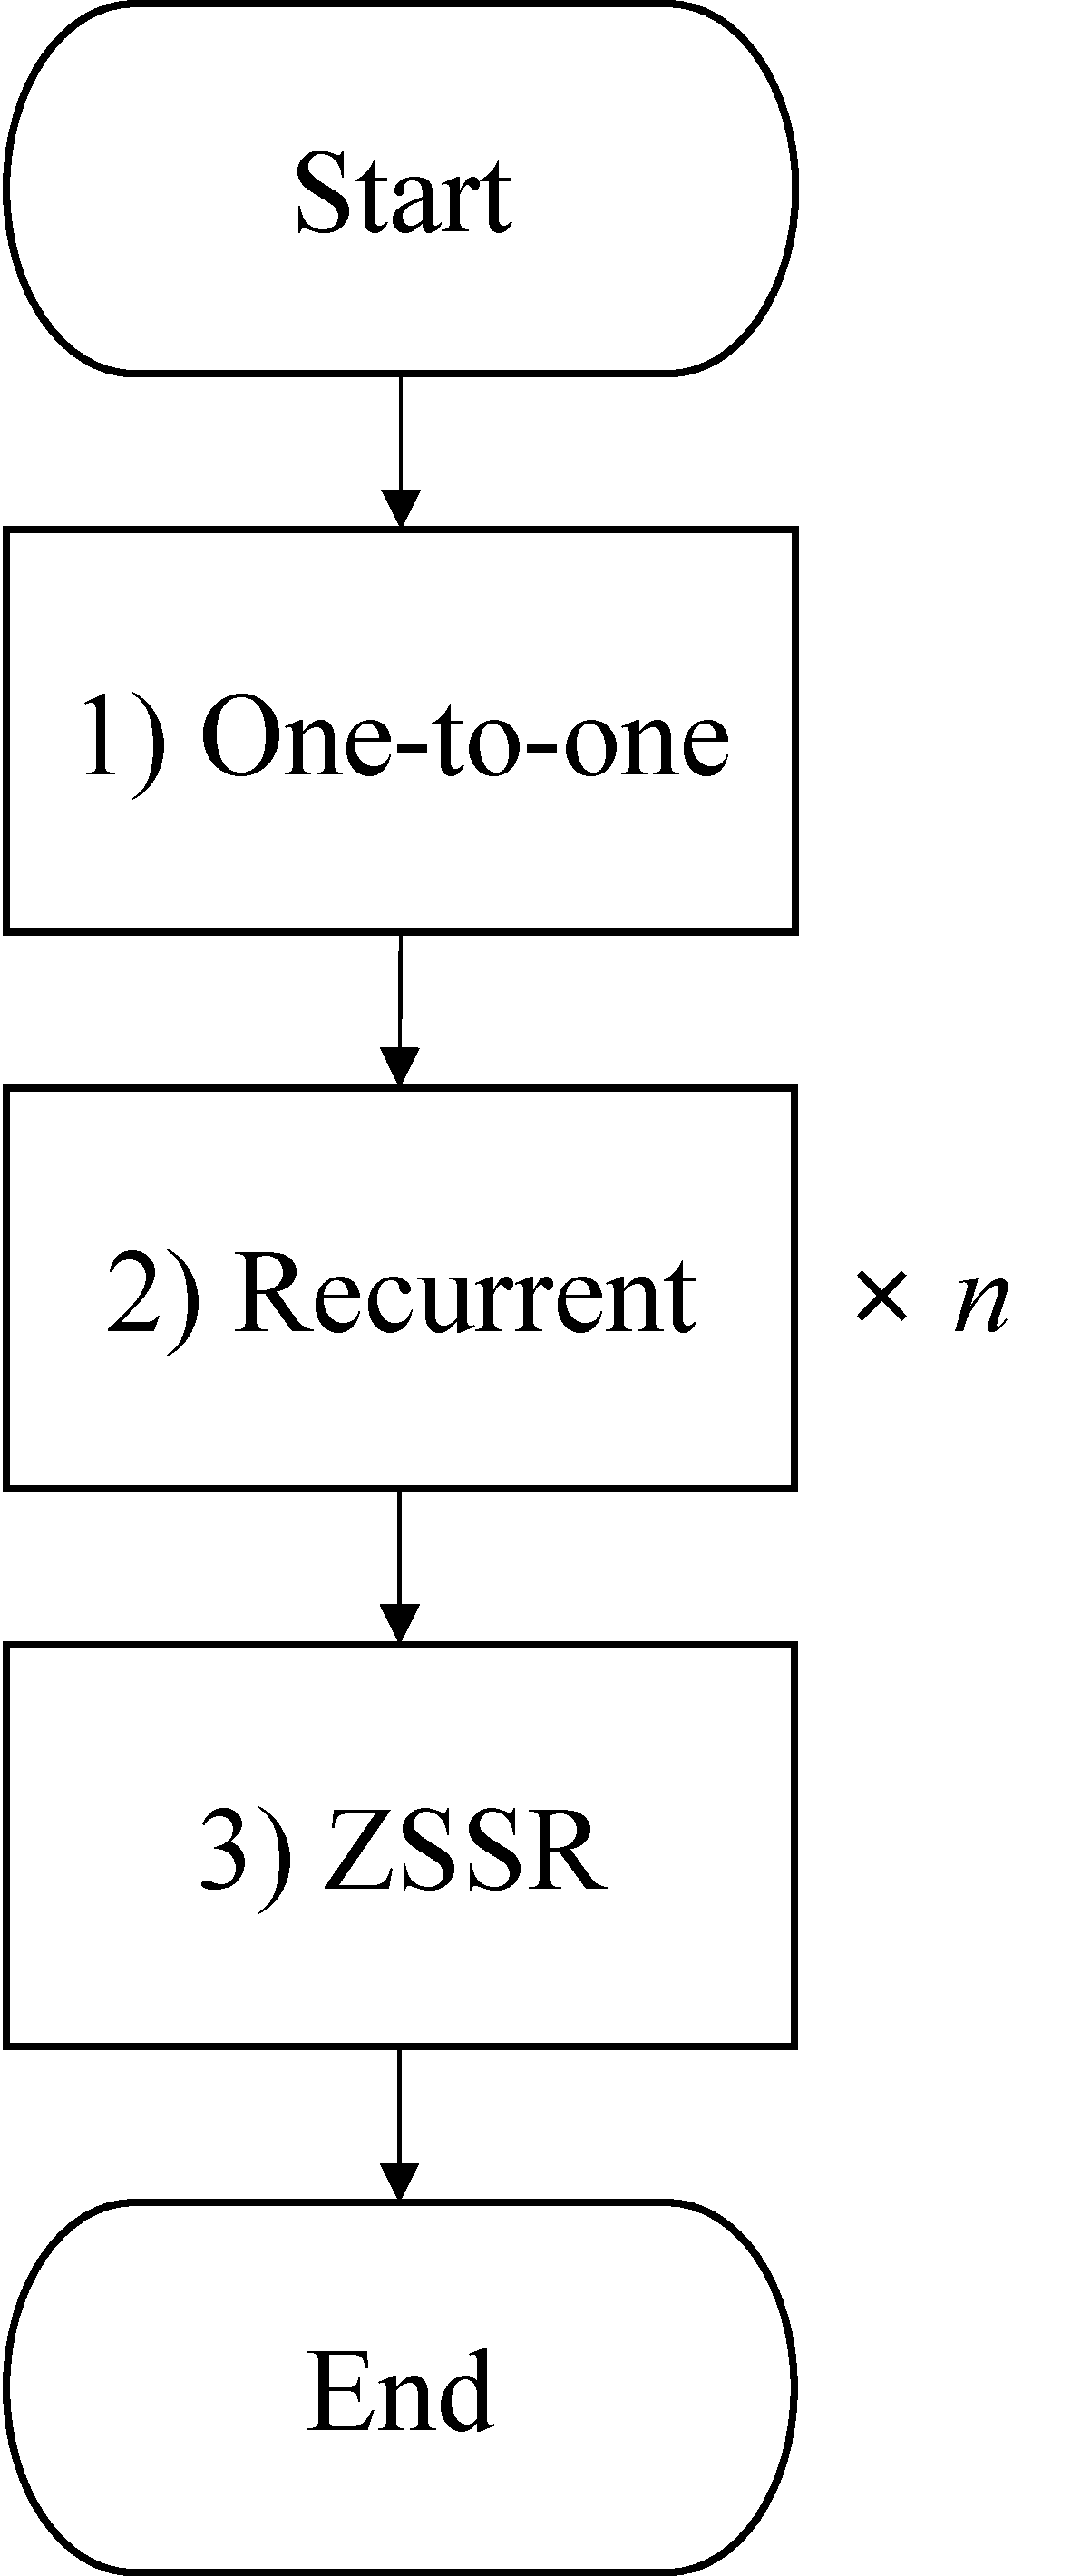
\includegraphics[width=0.3\columnwidth]{fig/Ryu-fig4.pdf}
    \caption{Overall framework of proposed image restoration method.}
    \label{fig:overall}
\end{figure}

\subsubsection{O2O}
O2O mapping learning is conducted in this study, in which one image is trained to follow the characteristics of another image. This allows the network to be trained such that the low-frequency images can mimic the characteristics of the high-frequency images. In this method, a deep neural network $\mathcal{D}$ with learning parameters $\Theta$ is trained to map an image at $\alpha$ THz, $I_\alpha$, to an image at $\beta$ THz, $I_\beta$. The objective of the training is to obtain the parameter $\Theta$ such that minimizes the loss between the output image $\mathcal{D}({I_\alpha};\Theta)$ generated through the network and target image $I_\beta$, as expressed in Equation~\ref{eq1}.

\begin{equation}
\argmin_{\Theta} \mathcal{L}(\mathcal{D}({I_\alpha};\Theta), I_\beta),
\label{eq1}
\end{equation}
where $\mathcal{L}$ denotes the loss function for supervised learning.

In this study, the network is trained using source images, with target images serving as the ground truth. During the inference, the input images used are called inference images. A network trained with $I_\alpha$ as the source and $I_\beta$ as the target is succinctly denoted as $\mathcal{D}_{I_\alpha\rightarrow I_\beta}$. The process of inferring an image at $\gamma$ THz, $I_\gamma$, using this model can be written as
\begin{equation}
\mathcal{D}_{I_\alpha\rightarrow I_\beta}(I_\gamma).
\end{equation}

Fig.~\ref{fig:o2o_explain} illustrates the training and inference procedures of the One-to-one method. Fig.~\ref{fig:o2o_explain}(a) shows the training process. As described earlier, based on $I_\alpha$ as the source and $I_\beta$ as the target, the network is trained to minimize the loss between the network output and target. Fig.~\ref{fig:o2o_explain}(b) shows the process of inferring an inference image $I_\gamma$, obtained within (intra) the THz SAHS images, using the trained network $\mathcal{D}_{I\alpha\rightarrow I_\beta}$, which is termed ``intra-data inference.'' As shown in Fig.~\ref{fig:o2o_explain}(c), the same network is used for cross-data inference, where a new image $J$, which is unrelated to the THz SAHS images used for training, is inferred. Image $J$ can exhibit a completely different form the training images and can be obtained using a system different from that used for the training images. This process is known to as ``cross-data inference.''

\begin{figure*}[htbp]
    \centering
    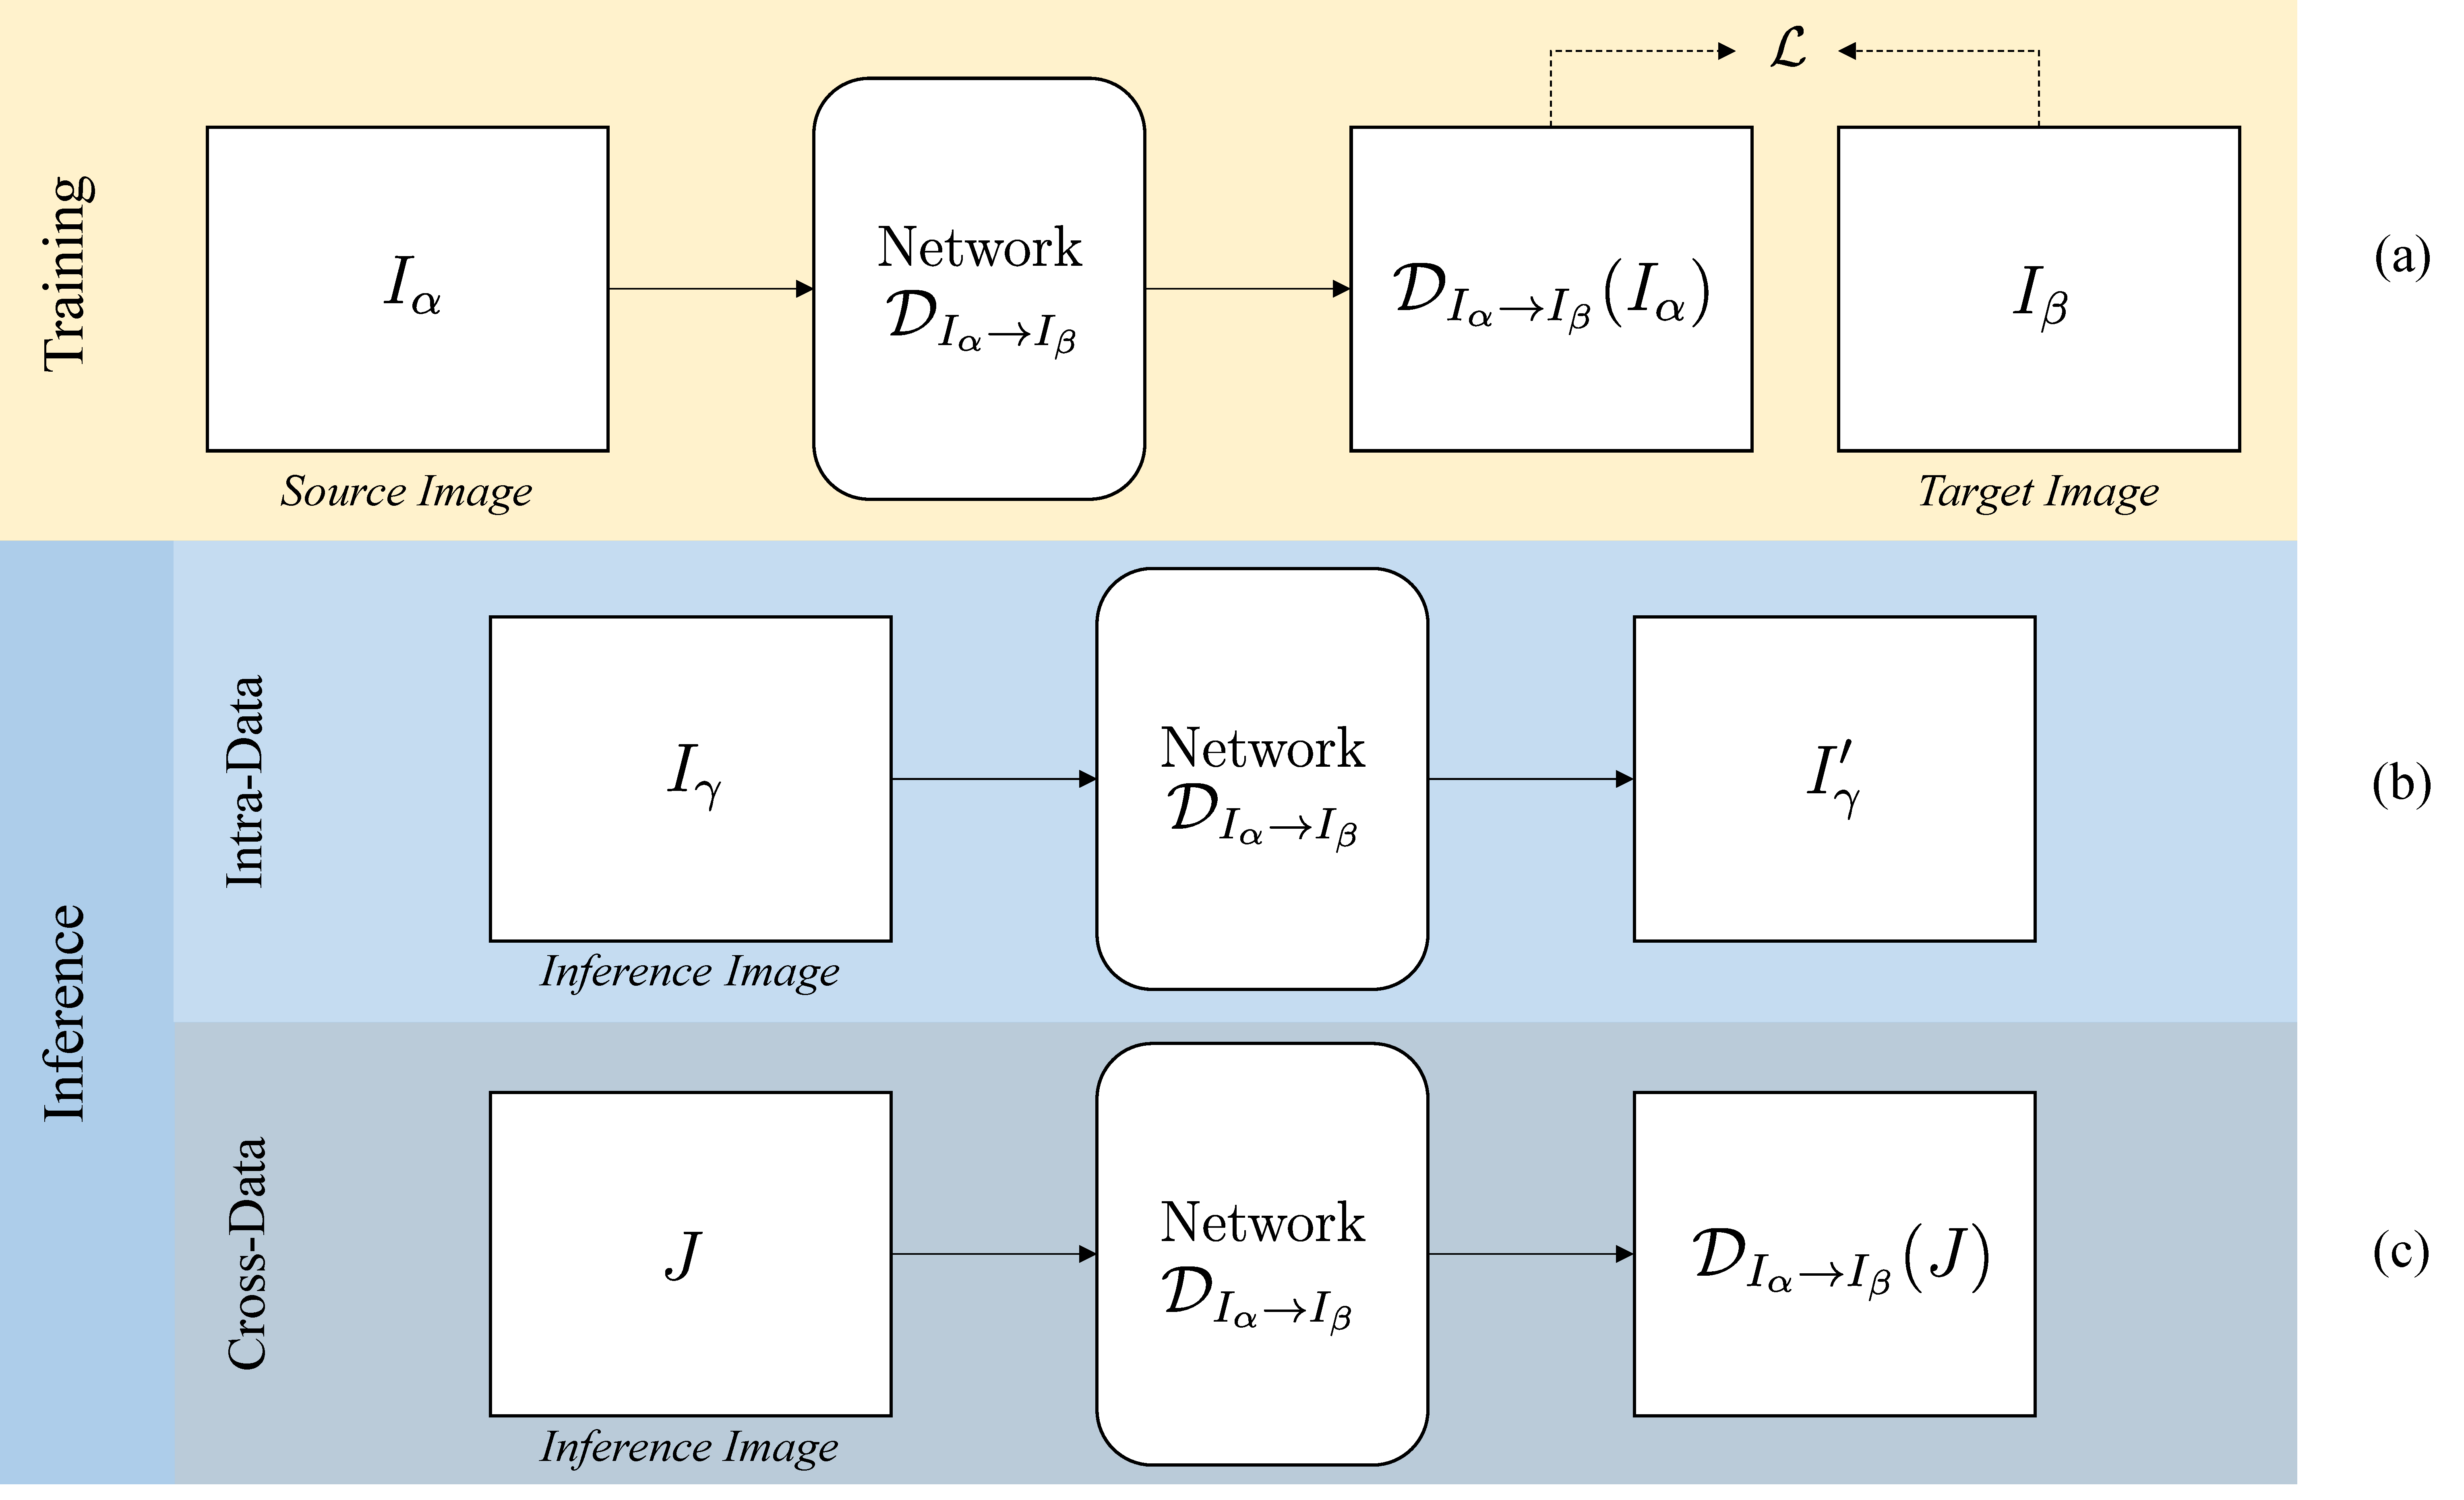
\includegraphics[width=0.7\textwidth]{fig/Ryu-fig5.pdf}
    \caption{O2O training and inference process. (a) Training; (b) inference with intra-data; (c) inference with cross-data.}
    \label{fig:o2o_explain}
\end{figure*}

The results of applying $I_\gamma$ vary depending on how $\alpha$ and $\beta$ are set. Using a model that maps from low to high frequency $(\alpha < \beta)$ enhances the spatial resolution of low-frequency images. This enhancement occurs because the blurry low-frequency images mimic the sharpness of the high-frequency images, thereby overcoming the diffraction limit of the low-frequency images. Conversely, mapping an image obtained from high-frequency with a weak signal in the THz-TDS system to an image obtained from low-frequency with a relatively stronger signal  $(\alpha > \beta)$ helps in reducing noise in high-frequency images, although this may introduce some blurring owing to the emulation of low-frequency images. The model trained as such can be applied to new THz images unrelated to the training data to enhance image sharpness or reduce noise. More detailed experimental results are presented in Section~\ref{sec:exp}.

\subsubsection{RE}
The image inferred using a network trained using the One-to-one method is used as a target for repeating the O2O training. This process, which is repeated $n$ times, allows for further improvements to the enhanced image and is abbreviated as RE.

After conducting One-to-one training, the result of inferring $I_\beta$ using the obtained model is denoted as $I_\beta'$. This can be expressed as shown in Equation~\ref{eq:o2o}.
\begin{equation}
\mathcal{D}_{I_\alpha\rightarrow I_\beta}(I_\beta) = I_\beta'.
\label{eq:o2o}
\end{equation}

Subsequently, it is used as a target and $I_\beta$ is used as a source for further training; next the model is used to infer $I_\beta'$. This result is denoted as $I_\beta''$, which can be expressed as shown in Equation~\ref{eq:re1}.
\begin{equation}
        \mathcal{D}_{I_\beta\rightarrow I_\beta'}(I_\beta') = I_\beta''.
        \label{eq:re1}
\end{equation}
This process can be repeated recurrently. However, as will be discussed in Section~\ref{sec:exp}, excessive repetition of this process can yield unnatural visual results. The result of performing RE twice can be expressed as shown in Equation~\ref{eq:re2}.
\begin{equation}
    \mathcal{D}_{I_\beta'\rightarrow I_\beta''}(I_\beta'') = I_\beta'''.
    \label{eq:re2}
\end{equation}

\begin{figure*}[htbp]
    \centering
    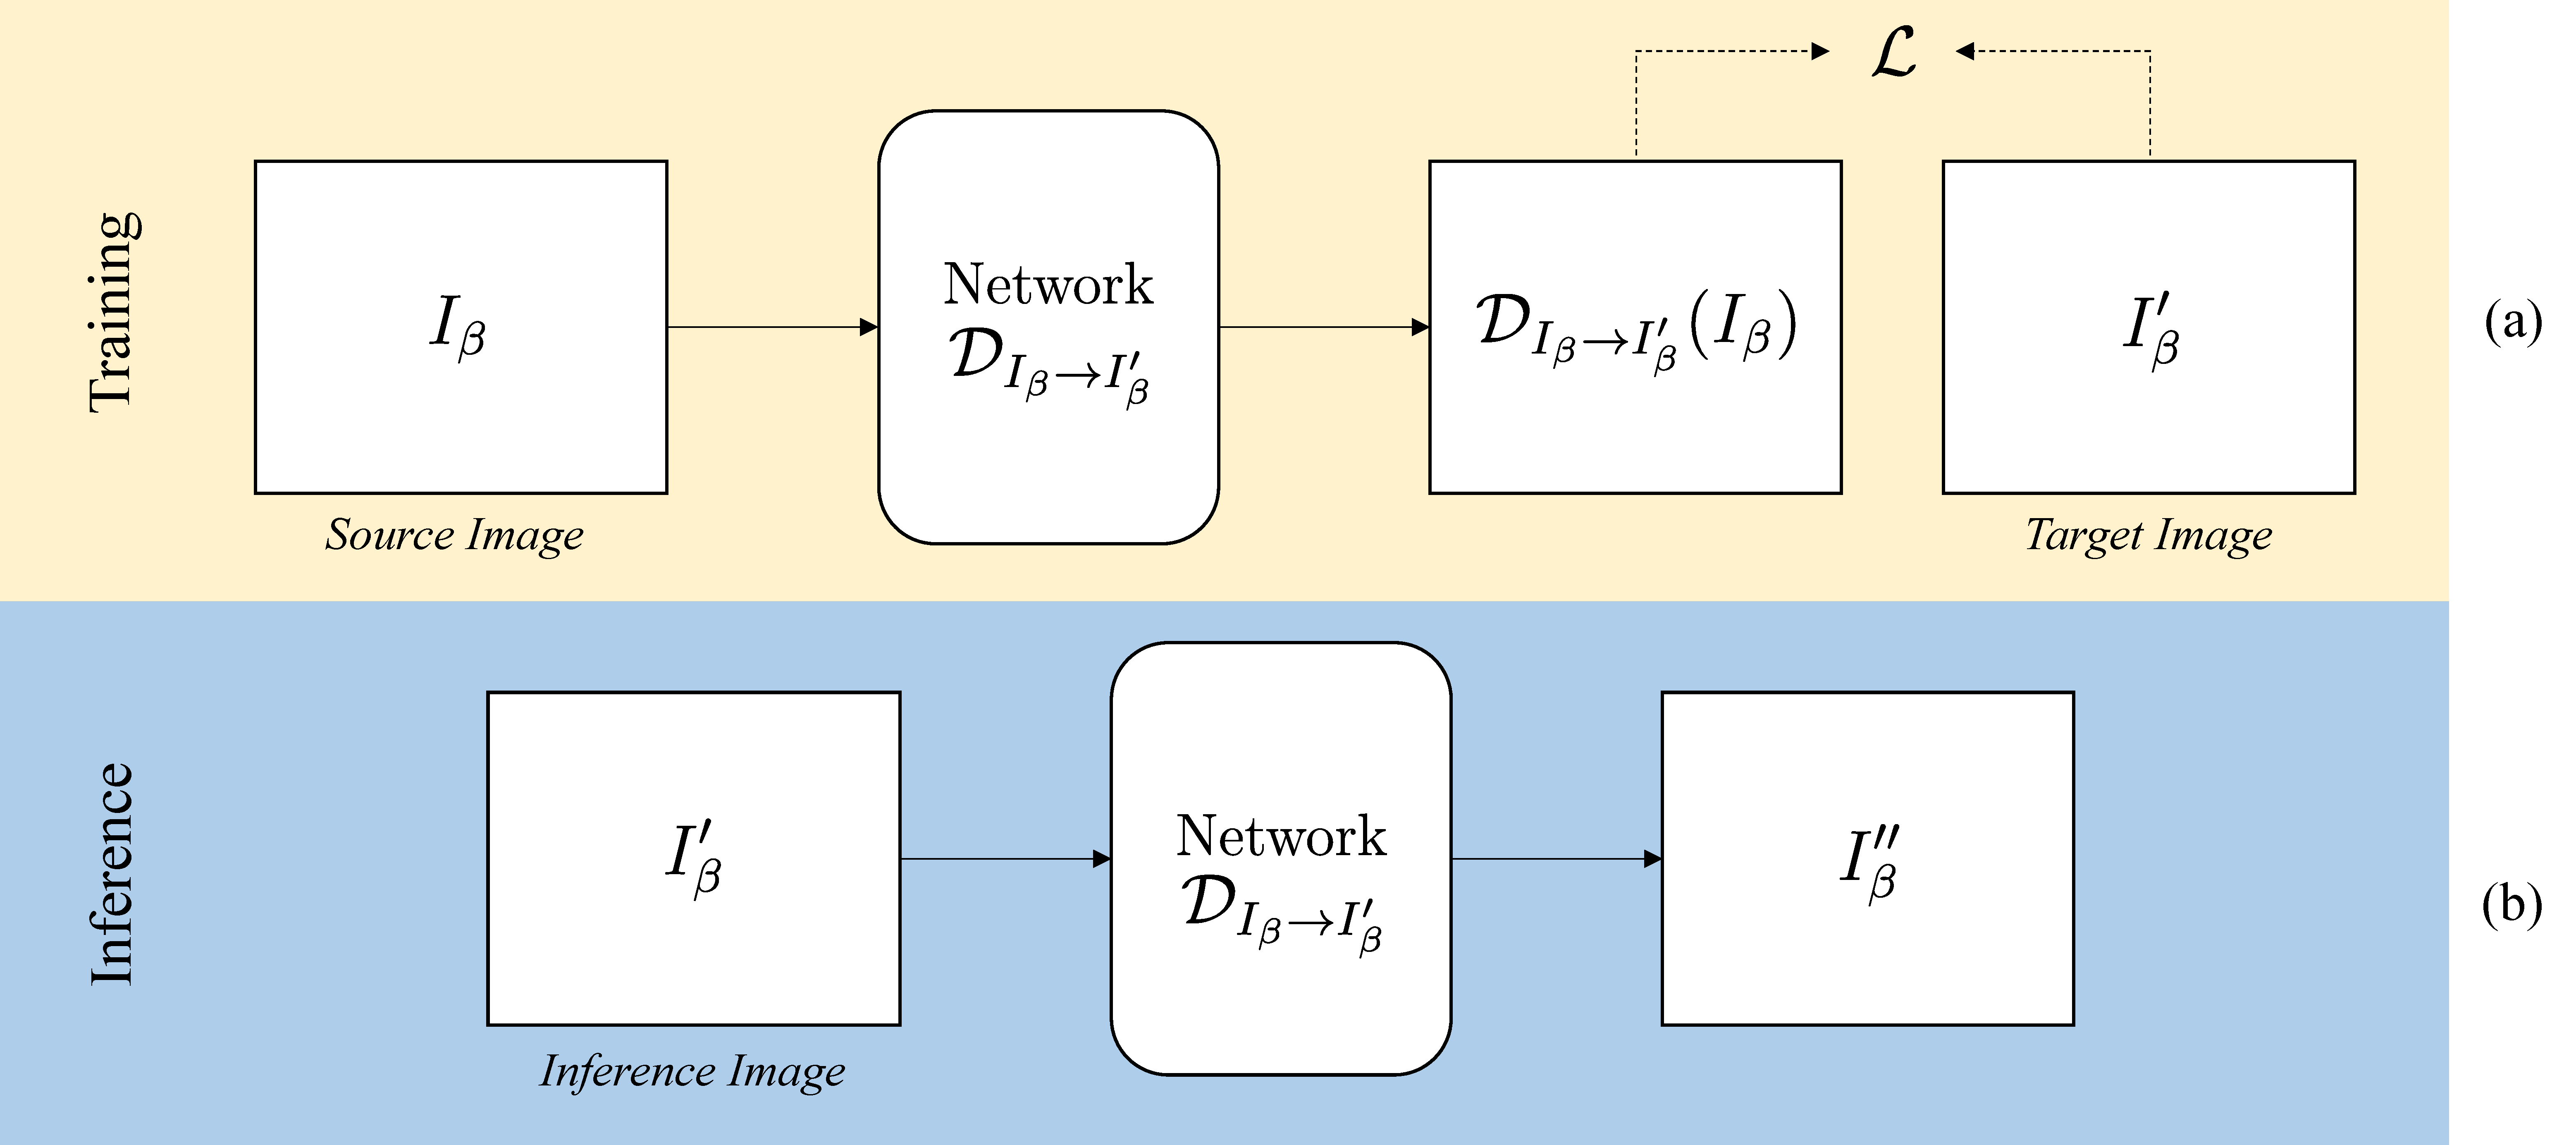
\includegraphics[width=0.7\textwidth]{fig/Ryu-fig6.pdf}
    \caption{RE training and inference process. (a) Training; (b) inference.}
    \label{fig:recurrent_explain}
\end{figure*}
Fig.~\ref{fig:recurrent_explain} shows the training and inference processes of the RE method. It involves the same procedure as O2O; however, the source and target images used are the target and inference results of O2O, respectively.


\subsubsection{ZSSR}
ZSSR is an unsupervised image SR method proposed in~\cite{shocher2018zssr}. Unlike traditional super-resolution methods, ZSSR operates without the need for pre-training on large external datasets. Instead, this method identifies patterns and structures repeated within a single input image and uses these findings as a basis to learn SR transformations. During inference, the model is dynamically trained, allowing the learned model to be immediately used to infer a high-resolution version of the input image. It can adapt to different image settings, thus enabling SR on old photographs, noisy images, biological data, and other images with unknown or non-ideal acquisition processes. The ability of this method to train on a single image renders it particularly suitable for THz images, in which accurately estimating blur and noise is challenging. In addition, because of the general difficulty in obtaining high-resolution THz images, applying ZSSR can yield the best quality images under the resources of the THz imaging system in use. Fig.~\ref{fig:zssr_explain} shows the training and inference processes involved in the ZSSR technique. The inference image $I$, initially downscaled by a scale factor $s$, is then used as the source, with $I$ as the target, to train the SR network. After training, the SR network's weights are used to infer $I$, thus resulting in an image with width and height increase by a factor of $s$.

\begin{figure*}[htbp]
    \centering
    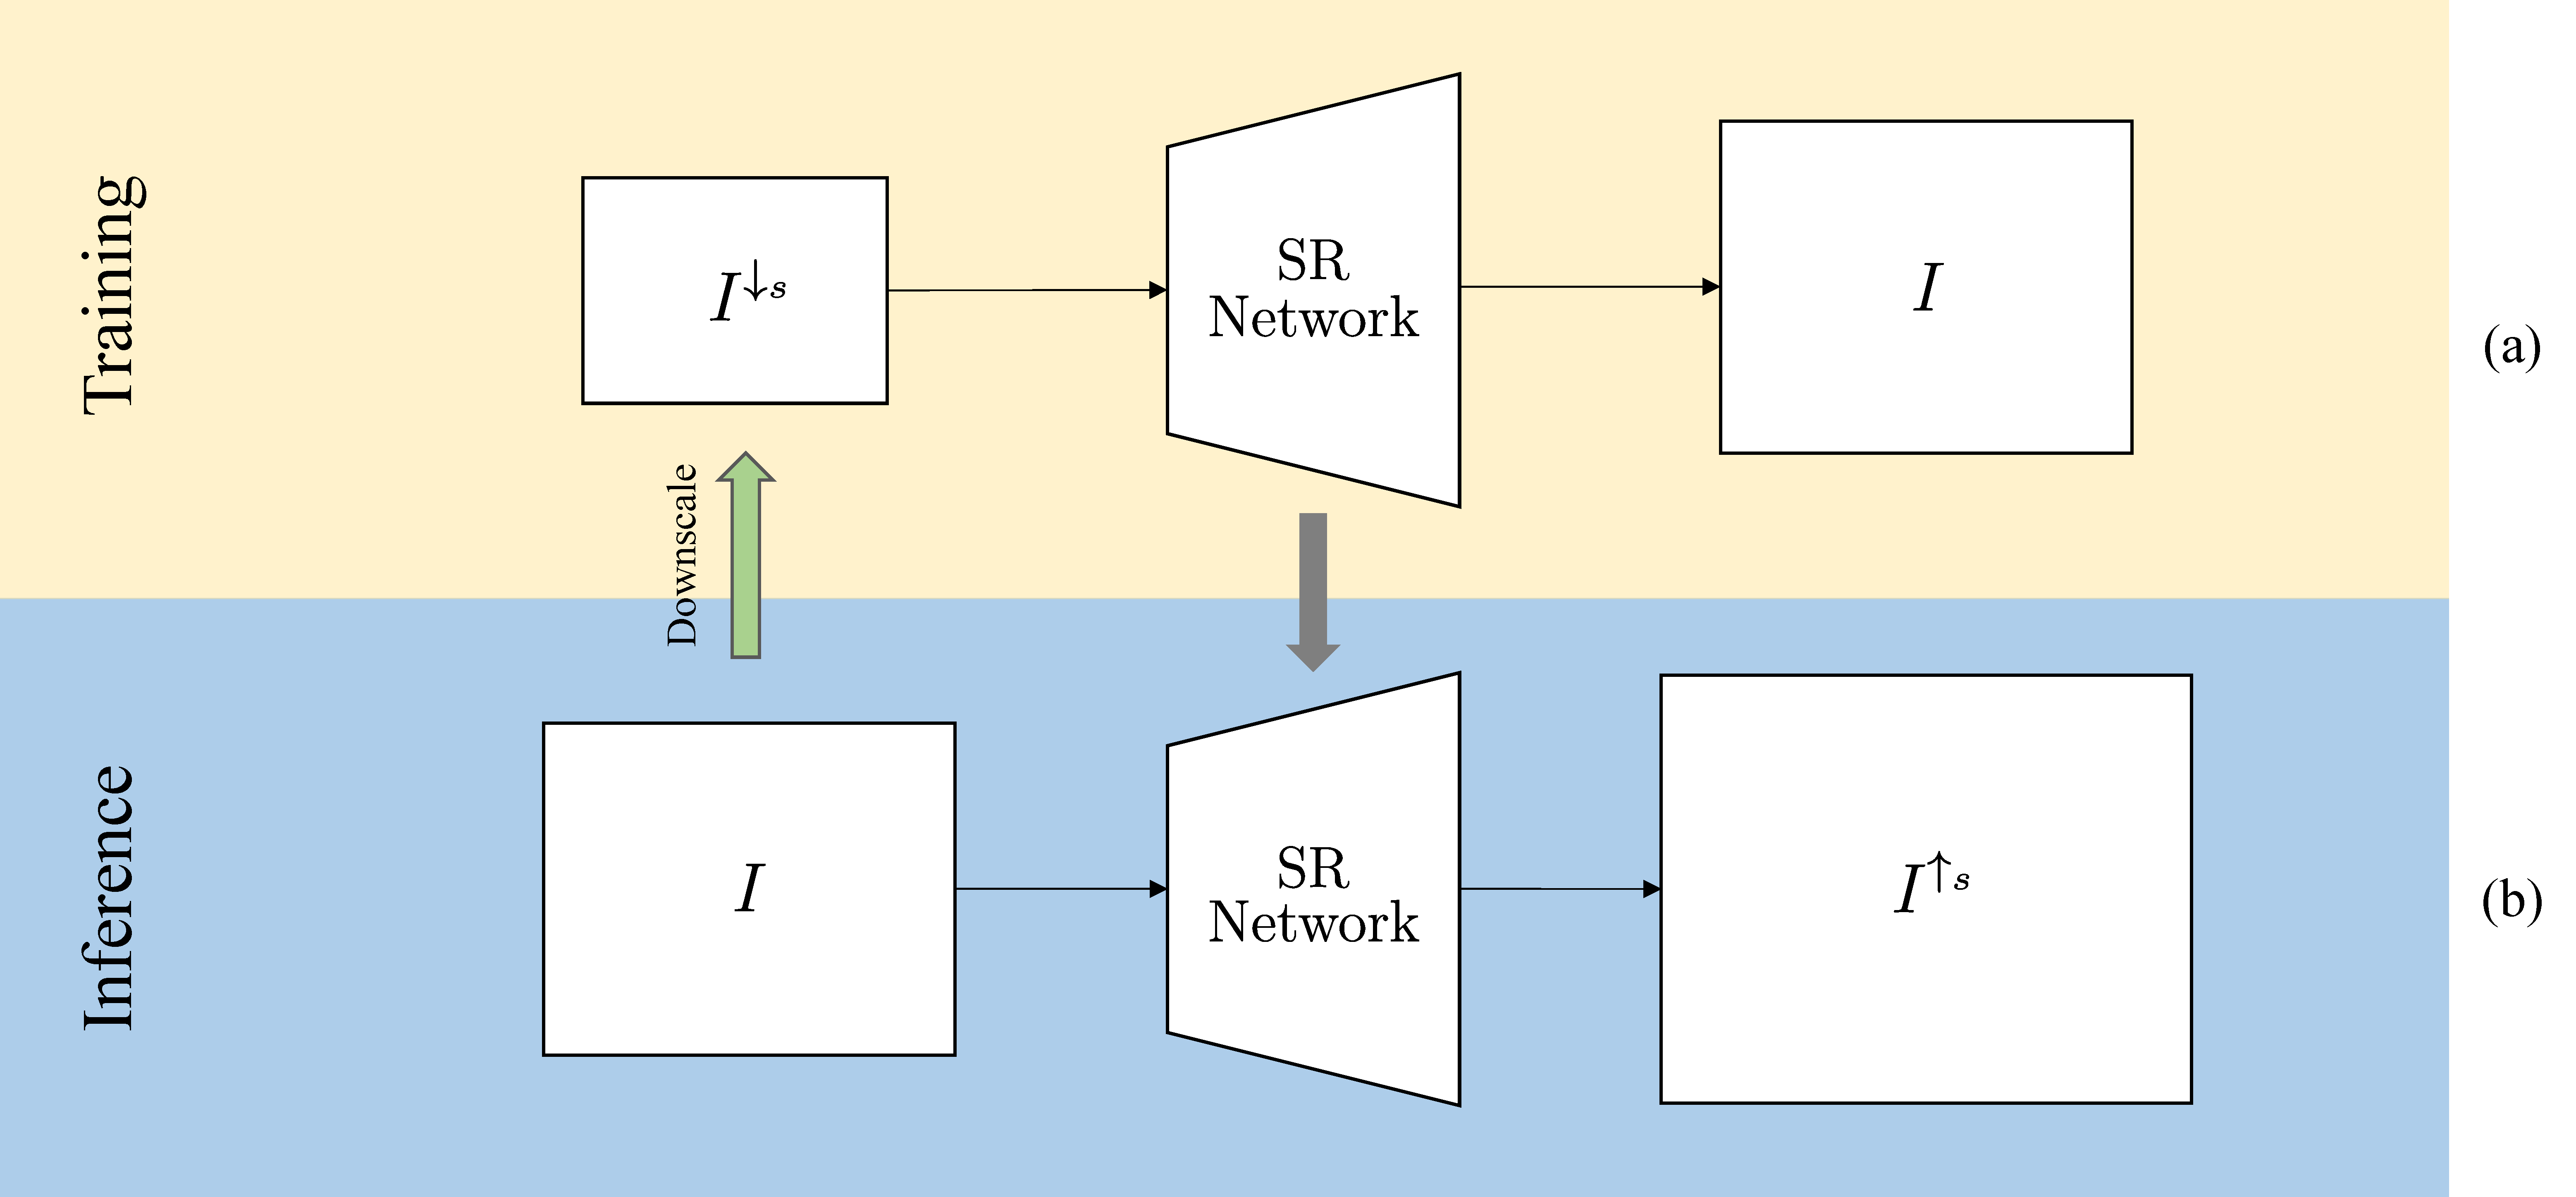
\includegraphics[width=0.65\textwidth]{fig/Ryu-fig7.pdf}
    \caption{ZSSR training and inference process. (a) Training; (b) inference.}
    \label{fig:zssr_explain}
\end{figure*}
\section{Experiments}
\label{sec:exp}
\subsection{Implementation details}
We utilized a simple and lightweight CNN for two reasons. The first is to demonstrate the effectiveness of the proposed method without depending on the complex network structure. The second reason pertains to the nature of the training process, which involves learning from a single pair of images at a time. In the typical image restoration training, a large dataset comprising multiple pairs of degraded and ground-truth images is used. In such cases, the training network tends to be deep and complex to capture the diversity of all possible pairs in the learned weights. However, the training in our proposed method involves either a single pair or a single image, thus resulting in significantly less diversity in relationships; therefore, a relatively smaller and simpler network is sufficient. Fig.~\ref{fig:network} shows the constructed network, which comprises eight hidden layers with 64 channels each. ReLU activation is applied to each layer, and the final layer features a skip connection linked to the input layer. In the ZSSR network, the only addition to the base network is an module that upsamples the input patch by a factor of n, as shown in Fig.~\ref{fig:network}. All the experiments were conducted on an NVIDIA A100 GPU using PyTorch~\cite{paszke2019pytorch}. We optimized the parameters of the network $\mathcal{D}$ by minimizing the $L_1$ pixel loss.
\begin{equation}
    \mathcal{L} = ||\mathcal{D}(I_{source}) - I_{target}||_1,
\end{equation}
where $I_{source}$ is the source image, and $I_{target}$ is the target image. During training, the patch size was set to $96\times96$. An Adam optimizer~\cite{kingma2014adam} with $\beta_1=0.9$ and $\beta_2=0.999$ was
used to train the network for 15,000 iterations. The learning rate was initially set to $1e^{-5}$ which decayed by 10 after 10,000 iterations.

The data used for training comprised THz SAHS images measured using a THz-TDS system based on the USAF 1951 resolution test chart. For each training session, we selected two frequencies from the THz SAHS image to establish input-target mapping.

\begin{figure}[ht]
    \centering
    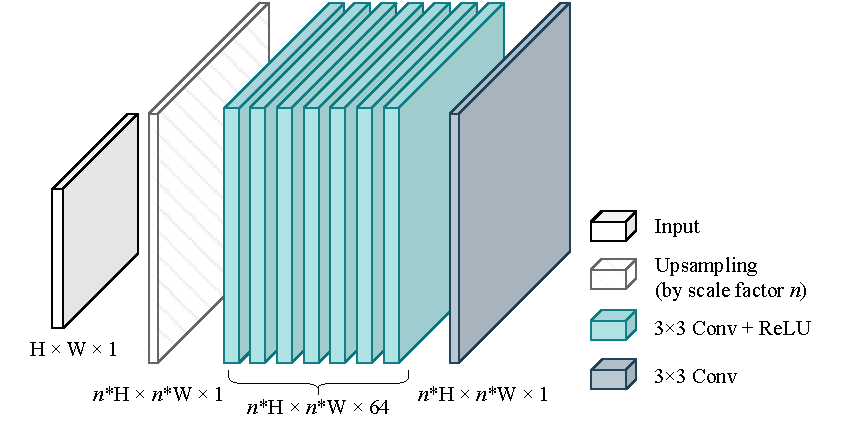
\includegraphics[width=\columnwidth]{fig/Ryu-fig8.pdf}
    \caption{Network architecture used in proposed image restoration framework. Upsampling module is used only for ZSSR training.}
    \label{fig:network}
\end{figure}

\subsection{Data Preprocessing}
To acquire THz SAHS images of the USAF 1951 resolution test chart, the THz-TDS system was used to measure time-domain pulse signals at each pixel composing the image. Each time-domain pulse signal was captured with 1000 points within a 30 ps time window, as shown in Fig.~\ref{fig:system}.
The THz-TDS imaging system employs a fast-scanning method to quickly acquire THz signals. To reduce the image acquisition time, the sample was propagated along a zigzag path and then reshaped into two dimensions based on the path. Because of the hardware limitations of the system in the zigzag scanning process, the pixels in the even and odd rows were not aligned precisely. To resolve this issue, the pixels in the odd rows were shifted by $1/5$ of a pixel to align them with those in the even rows. Additionally, areas with pixel values of 0 around the image edges were removed, i.e., only significant regions of the data were used for training. The time-domain signal data of all pixels measured via THz-TDS were converted into frequency data using the FFT to acquire SAHS images. To perform training, all the pixel intensity values were normalized to between 0 and 255. Fig.~\ref{fig:tds_freq_point} shows the time- and frequency-domain signals of the most intense THz signal pixel in the THz SAHS image, and a 2.0 THz image measuring $282\times282$ pixels. Figs.~\ref{fig:tds_freq_point}a and b show the THz time-domain signal measured at the red dot shown in the 2 THz image in Fig.~\ref{fig:tds_freq_point}c, and the corresponding frequency-domain signal obtained via FFT, respectively.

\begin{figure}[htbp]
    \centering
    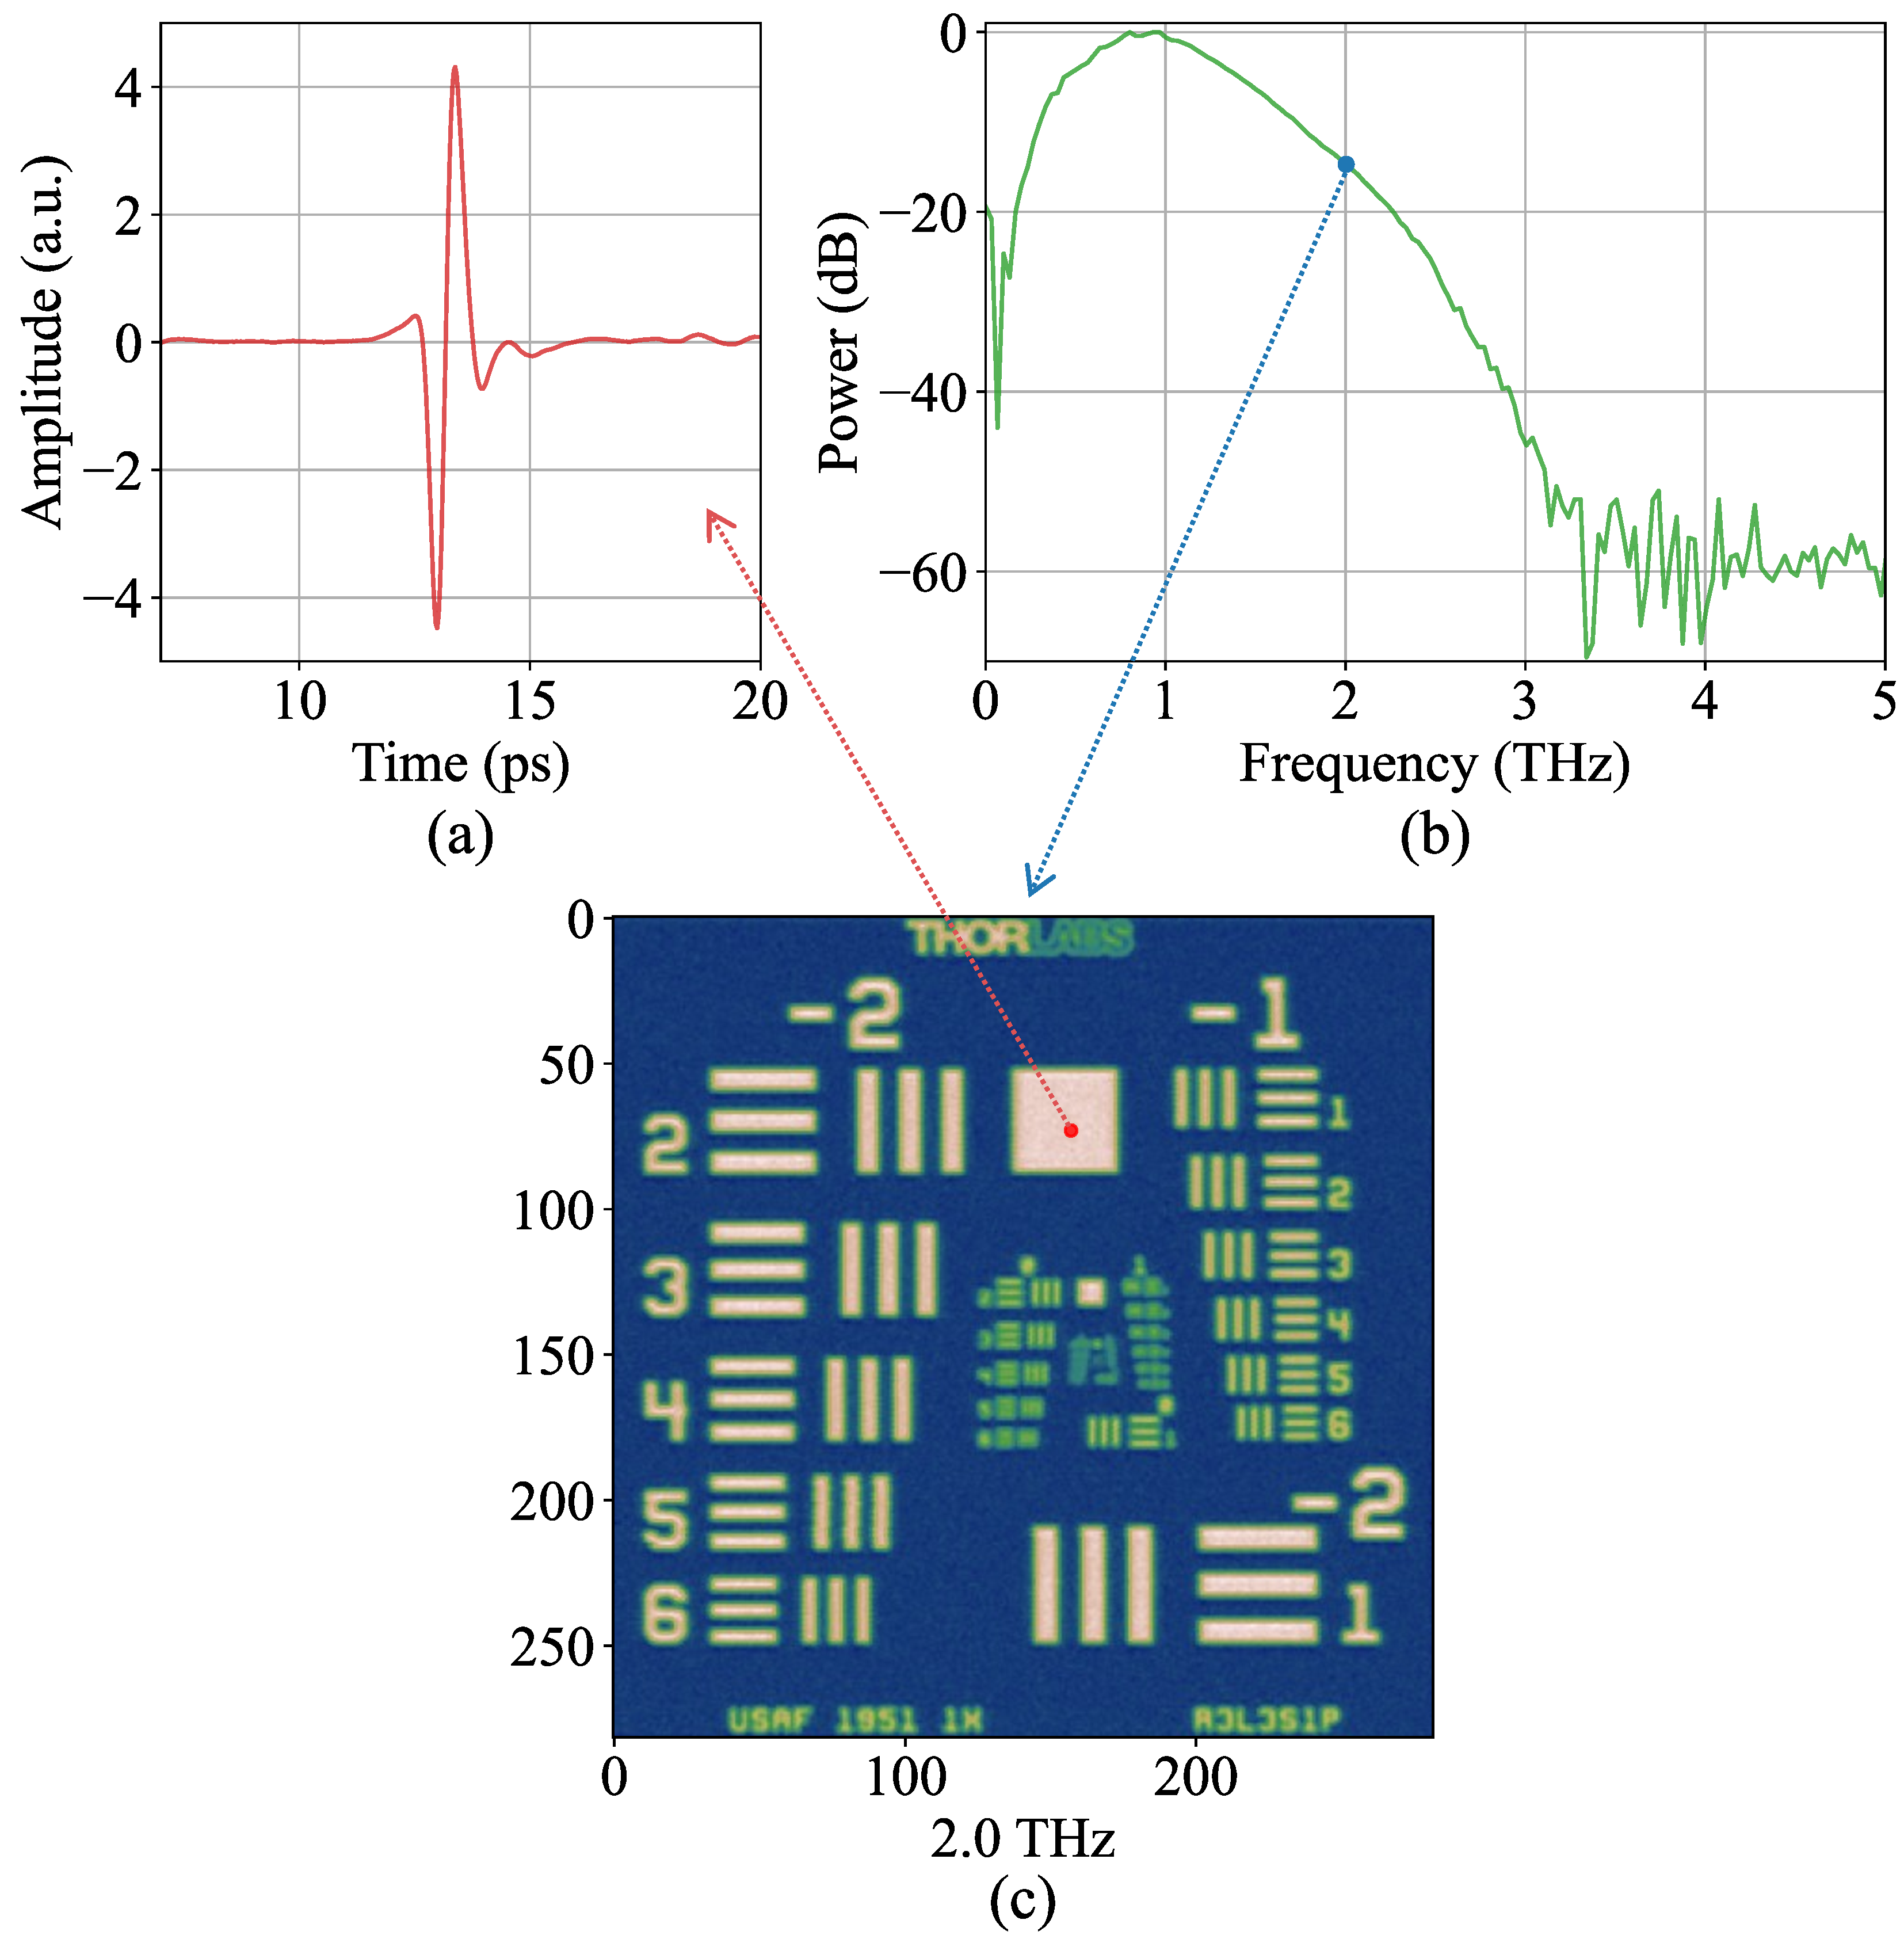
\includegraphics[width=\columnwidth]{fig/Ryu-fig9.pdf}
    \caption{Example of THz data. (a) Maximum power time-domain data (red point at (c)); (b) frequency-domain data; (c) 2.0 THz image (blue point at (b)).}
    \label{fig:tds_freq_point}
\end{figure}

\subsection{Self-Supervised Intra-Data Inference}
\label{sec:intra}
\begin{figure*}[htbp]
    \centering
    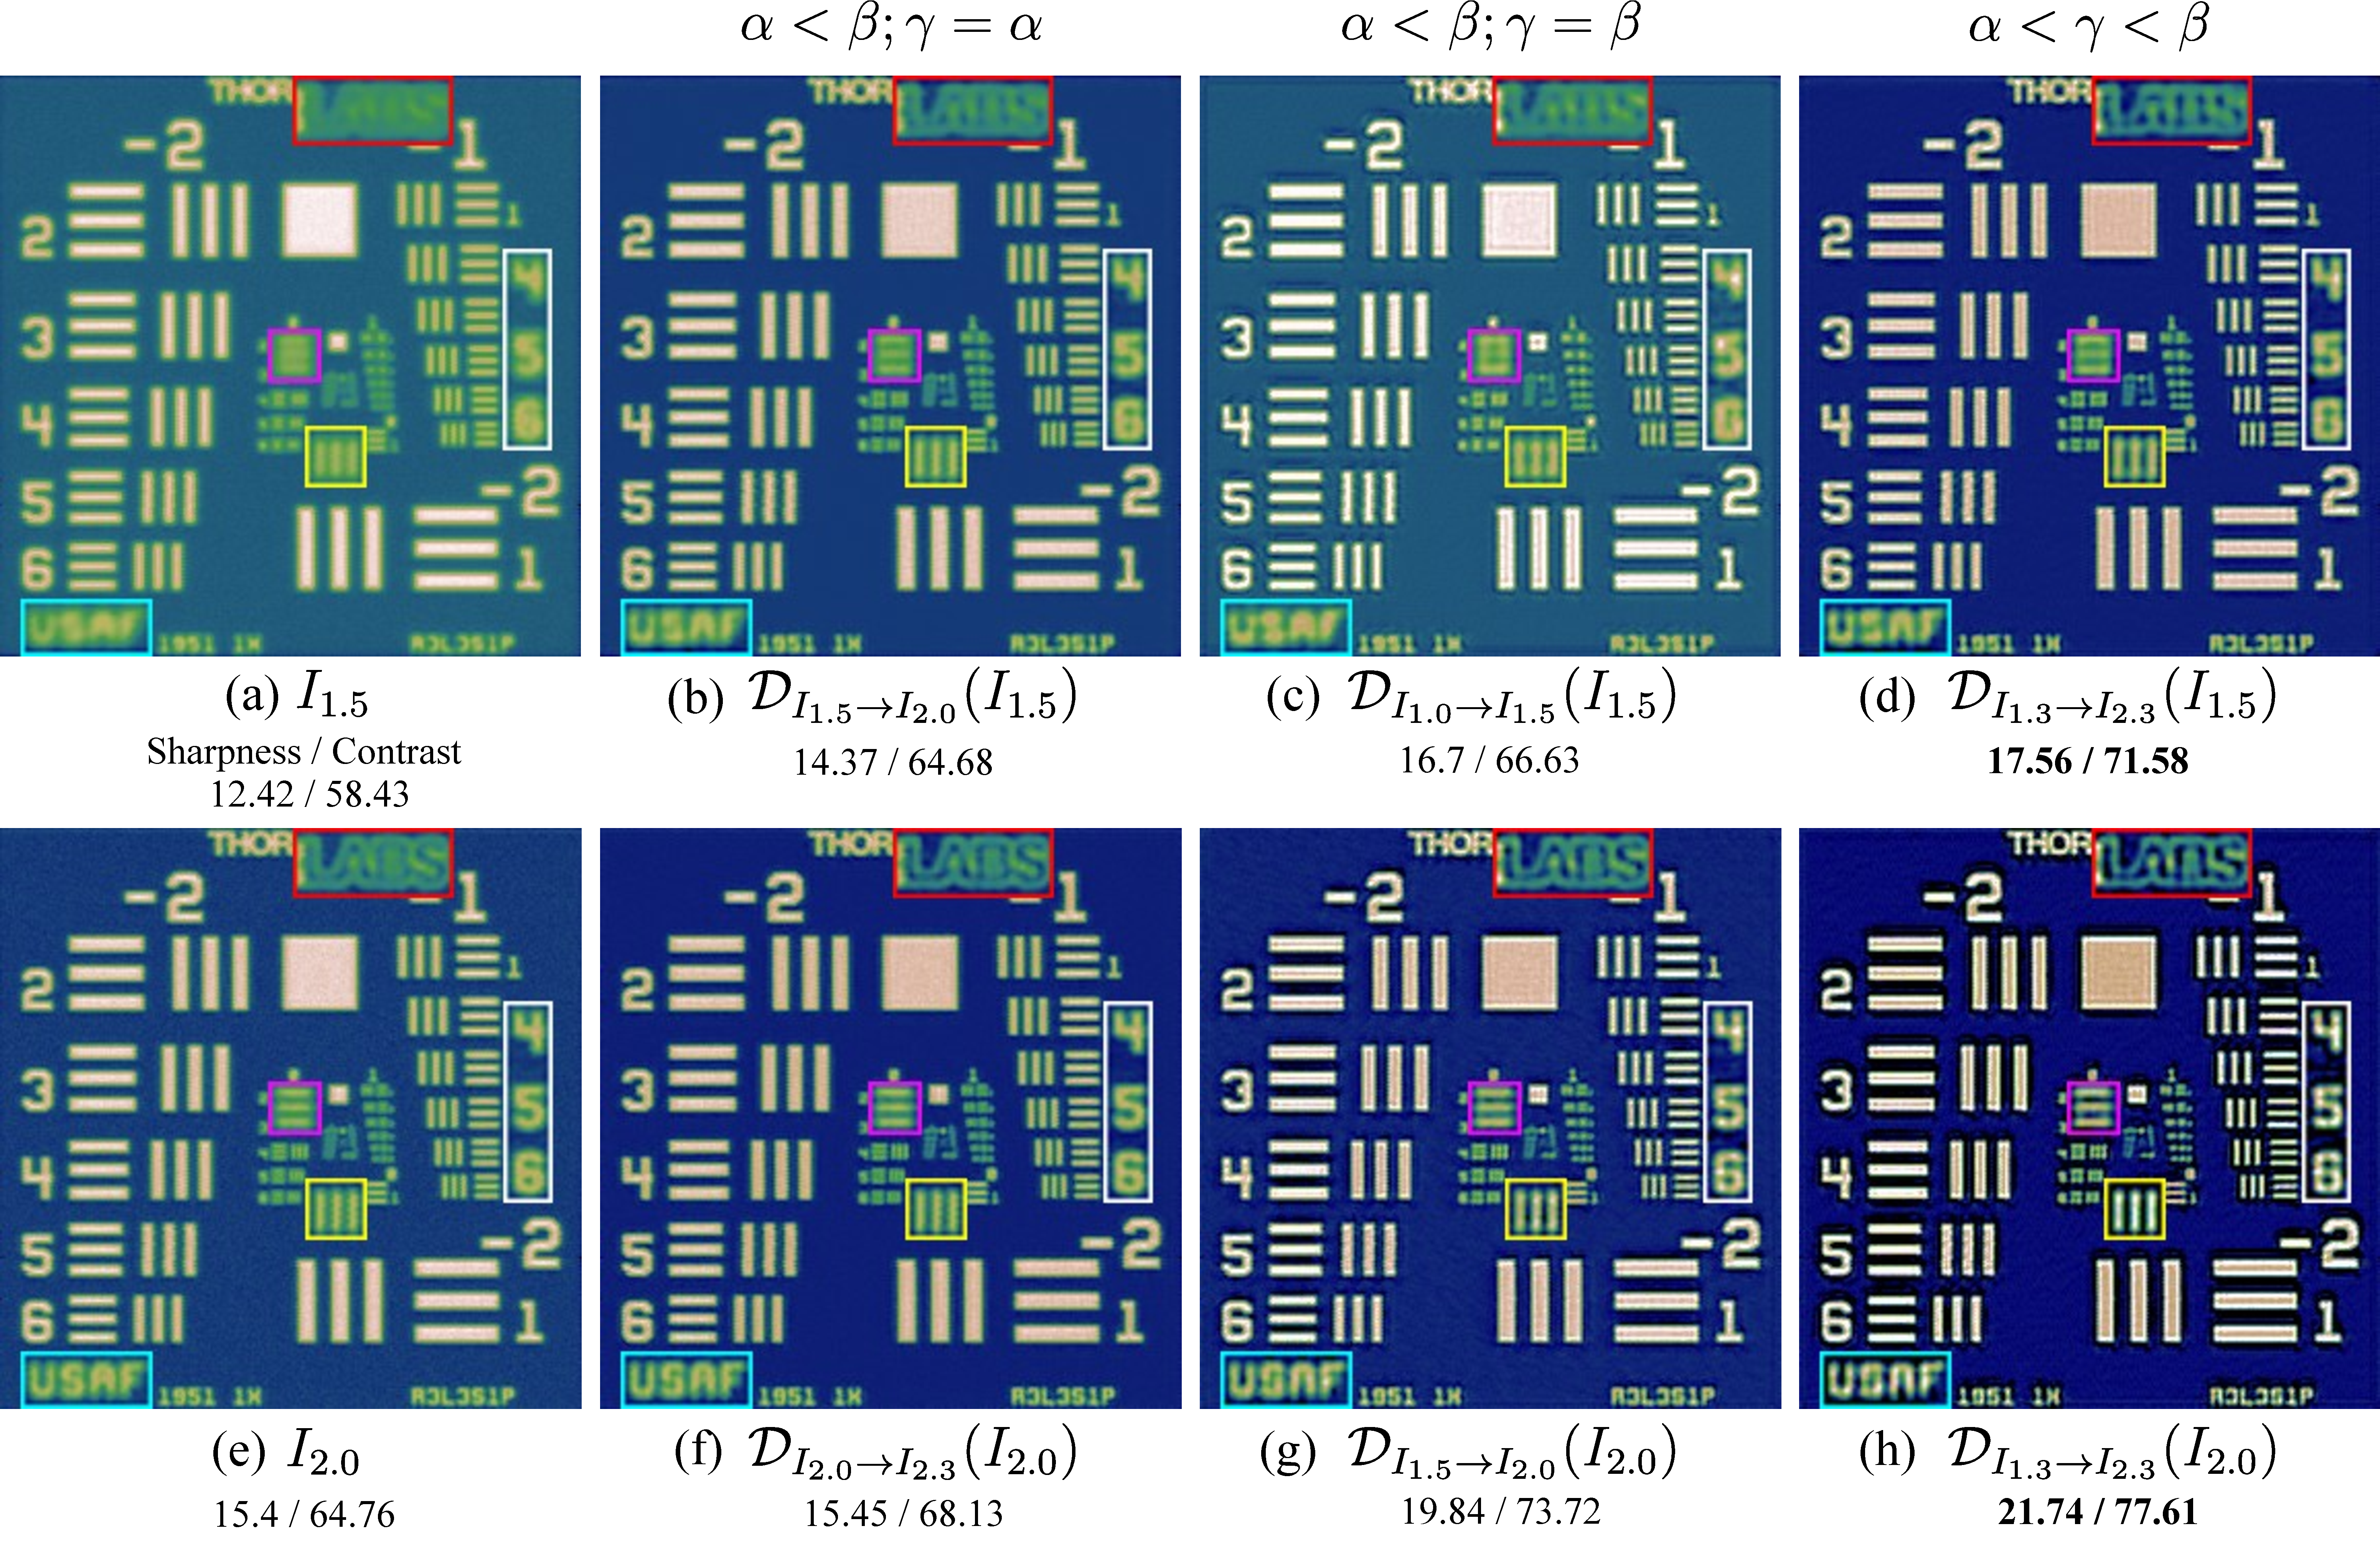
\includegraphics[width=\textwidth]{fig/Ryu-fig10.pdf}
    \caption{Self-supervised intra-data inference deblurring results based on 1.5 and 2.0 THz images. (a) Original 1.5 THz image; (b)-(d) O2O results of 1.5 THz image; (e) original 2.0 THz image; (f)-(h) O2O results of 2.0 THz image.}
    \label{fig:o2o_deblur}
\end{figure*}

The enhancement in image quality was demonstrated by applying the model trained using the O2O method, as depicted in Fig.~\ref{fig:o2o_explain}b, to the images used for training. It illustrates how low-frequency images emulate high-frequency images, thereby overcoming the diffraction limits of low-frequency images. During training, the frequencies of the input and target images are denoted as $\alpha$ and $\beta$, respectively; meanwhile, for inference, the frequency of the input image is denoted as $\gamma$. Generally, if $\alpha < \beta$ during network training, then blurriness can be eliminated by overcoming the low-frequency characteristics. Because high-frequency images exhibit higher sharpness than low-frequency images (see Fig.~\ref{fig:iqa}), learning this mapping can enhance the clarity of the image. However, high-frequency images above a certain frequency may exhibit higher noise levels; therefore, although the sharpness increases, additional noise may be introduced.

Fig.~\ref{fig:o2o_deblur} presents the visual results showing the overcoming of the diffraction limit of low-frequency images for 1.5 THz and 2.0 THz images. Figs.~\ref{fig:o2o_deblur} a and (e) are the original images before model inference, and Figs.~\ref{fig:o2o_deblur} (b) and (f) show the cases where $\gamma=\alpha$, which implies that the frequencies of the source and inference images are identical. Figs.~\ref{fig:o2o_deblur} (c) and (g) show the scenarios where $\gamma=\beta$, which implies that the inference and target image frequencies are the same. Finally, Figs.~\ref{fig:o2o_deblur} (d) and (h) show the results when the frequencies of the source, target, and inference images are different. The corresponding sharpness and contrast values are indicated below each image. As shown in Fig.~\ref{fig:o2o_deblur} a, the magnified area of the original 1.5 THz image exhibited blurry and smudged characteristics. The enhanced images (Figs.~\ref{fig:o2o_deblur} (b)-(d)) showed significantly clearer characteristics and more defined bar indices (see yellow box).  When the frequency of the inference image matched that of the source image, the image quality improved stably, as shown in Fig.~\ref{fig:o2o_deblur} (b). As shown in Fig.~\ref{fig:o2o_deblur} (c), when the frequency of the inference image matched that of the target, the clarity of the image clearly improved, however, it was accompanied by some distortion. Moreover, as shown in Fig.~\ref{fig:o2o_deblur} (d) and (h), when the inference image frequency of the source and target were different, the maximum sharpness and contrast was achieved at a specific frequency. This indicates the importance of selecting the appropriate frequency for the source and target images to enhance the quality of the inference image. The quantitative measures, such as sharpness and contrast, improved differently depending on the frequency matching in the inference results of the 1.5 THz image. When the frequency of the inference image matched that of the source image, the sharpness increased from 12.42 to 14.37, and the contrast increased from 58.43 to 64.68. When the frequency of the inference image matched that of the target, the sharpness and the contrast increased to 16.7 and 66.63, respectively. Finally, at a specific frequency different from those of both the source and target, the sharpness and contrast peaked at 17.56 and 71.58, respectively. Although some distortions occurred with the increased sharpness and contrast, the results were visually pleasant. In particular, Fig.~\ref{fig:o2o_deblur} (d) shows much less blurring compared with Fig.~\ref{fig:o2o_deblur} (a), which resulted in clearer and more defined characters. A similar trend was observed for the 2.0 THz image shown in Fig.~\ref{fig:o2o_deblur} (e).
The 2.0 THz image, owing to its frequency characteristics, was sharper and exhibited higher contrast than the 1.5 THz image. The trend identified in the inference results of the 1.5 THz image was correspondingly observed in the inference results of the 2.0 THz image.
At 2.0 THz, when the frequency of the inference image matched that of the source, the sharpness increased slightly from 15.4 to 15.45, and the contrast increased significantly from 64.76 to 68.13. Based on matching with the target image frequency, the sharpness and contrast increased substantially to 19.84 and 73.72, respectively. Notably, at a specific frequency different from those of both the source and target, the 2.0 THz image achieved the maximum sharpness and contrast values of 21.74 and 77.61, respectively. Matching the frequency of the inference image to that of the source resulted in stable and distortion-free image quality enhancement. However, performing inference at a frequency matching that of the target or one that is different from those of both the source and target can significantly improve image sharpness and contrast. These results emphasize the importance of selecting the appropriate frequency when generating inference images and show that, remarkably, when the frequency of the inference image matches that of the target image, or a specific frequency is chosen arbitrarily, significant improvements in image quality can be achieved. However, some degree of image distortion may occur.


\subsection{Self-Supervised Cross-Data Inference}
Next, we demonstrate that the proposed method can overcome the diffraction limit on images not used for training, as shown in Fig.~\ref{fig:o2o_explain}(c).
We inferred a new image $J$ (unrelated to the images used for training the model), which was trained with a positive USAF 1951 resolution target image. 
To ensure stable image-quality improvement, the frequency $\gamma$ of the inference image $J$ was set to be equal or similar to the frequency $\alpha$ of the input image used for training.
Fig.~\ref{fig:o2o_deblur_cross}(a) shows an optical image of the metal bookmark with a Korean Goryeo celadon shape, and Fig.~\ref{fig:o2o_deblur_cross}(b) presents a 1.0 THz image of the bookmark acquired using the same THz-TDS system. Figs.~\ref{fig:o2o_deblur_cross}(c)-(e) show the cross-data inference results from the trained model $\mathcal{D}$, which was trained on a USAF THz SAHS image. 
These results show a clear improvement in all the original THz images, both in terms of visual appearance as well as quantitatively in terms of sharpness and contrast values. Notably, inference using a model trained to map from 1.0 to 1.5 THz sharpened the image details and increased the contrast, thus resulting in a more distinct image. A model trained to map from 1.0 to 2.5 THz further accentuated these features, as the greater the frequency ratio between the source and target images, the more excessively it emulates the characteristics of the high-frequency image. As shown in Fig.~\ref{fig:o2o_deblur_cross}(e), selecting the appropriate frequencies for source and target images can enhance image quality. Like the intra-data inference, the cross-data inference allows one to improve image quality while adjusting the degree of image distortion by selecting appropriate $\alpha$ and $\beta$ values.

In this study, we validated that the application of a model trained using THz SAHS image data to new THz images can enhance visual quality, sharpness, and contrast. This model, which was trained to emulate the characteristics from low to high frequencies, demonstrated potential for wide application in various imaging systems. Additionally, the proposed method improves the quality beyond the diffraction limit of THz images, thus rendering it promising for applications in fields such as security inspection, medical imaging, and materials science.

\begin{figure*}[htbp]
    \centering
    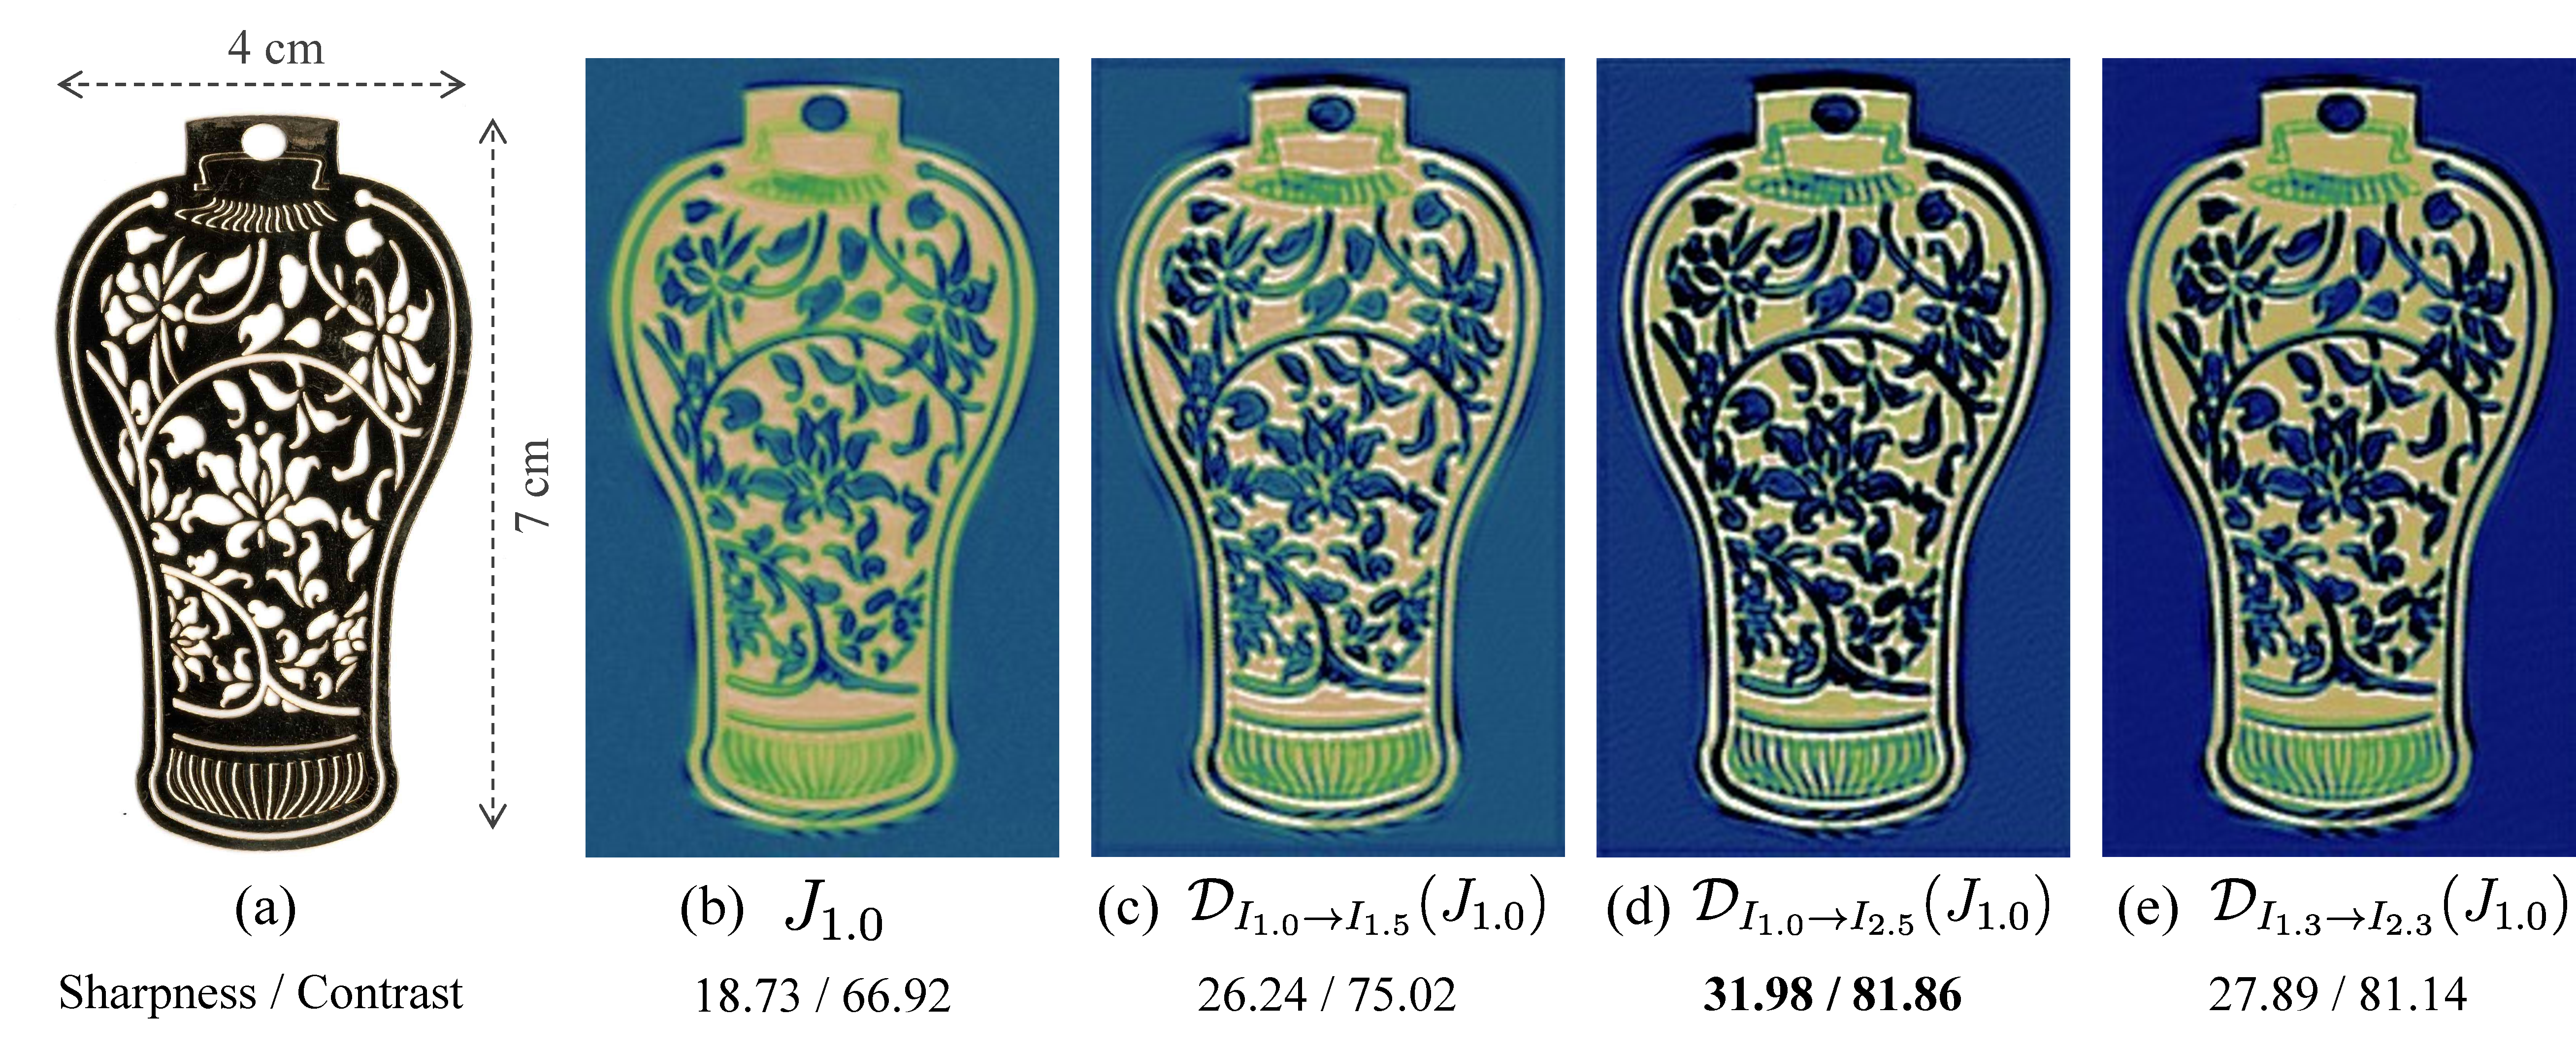
\includegraphics[width=\textwidth]{fig/Ryu-fig11.pdf}
    \caption{Self-supervised cross-data inference deblurring results based on O2O method. (a) Metal bookmark optical image; (b) measured THz image of metal bookmark at 1.0 THz; (c)-(e) cross-data inference results using pretrained model $\mathcal{D}$.}
    \label{fig:o2o_deblur_cross}
\end{figure*}

\subsection{High-Frequency Image Denoising}

\begin{figure*}[htbp]
    \centering
    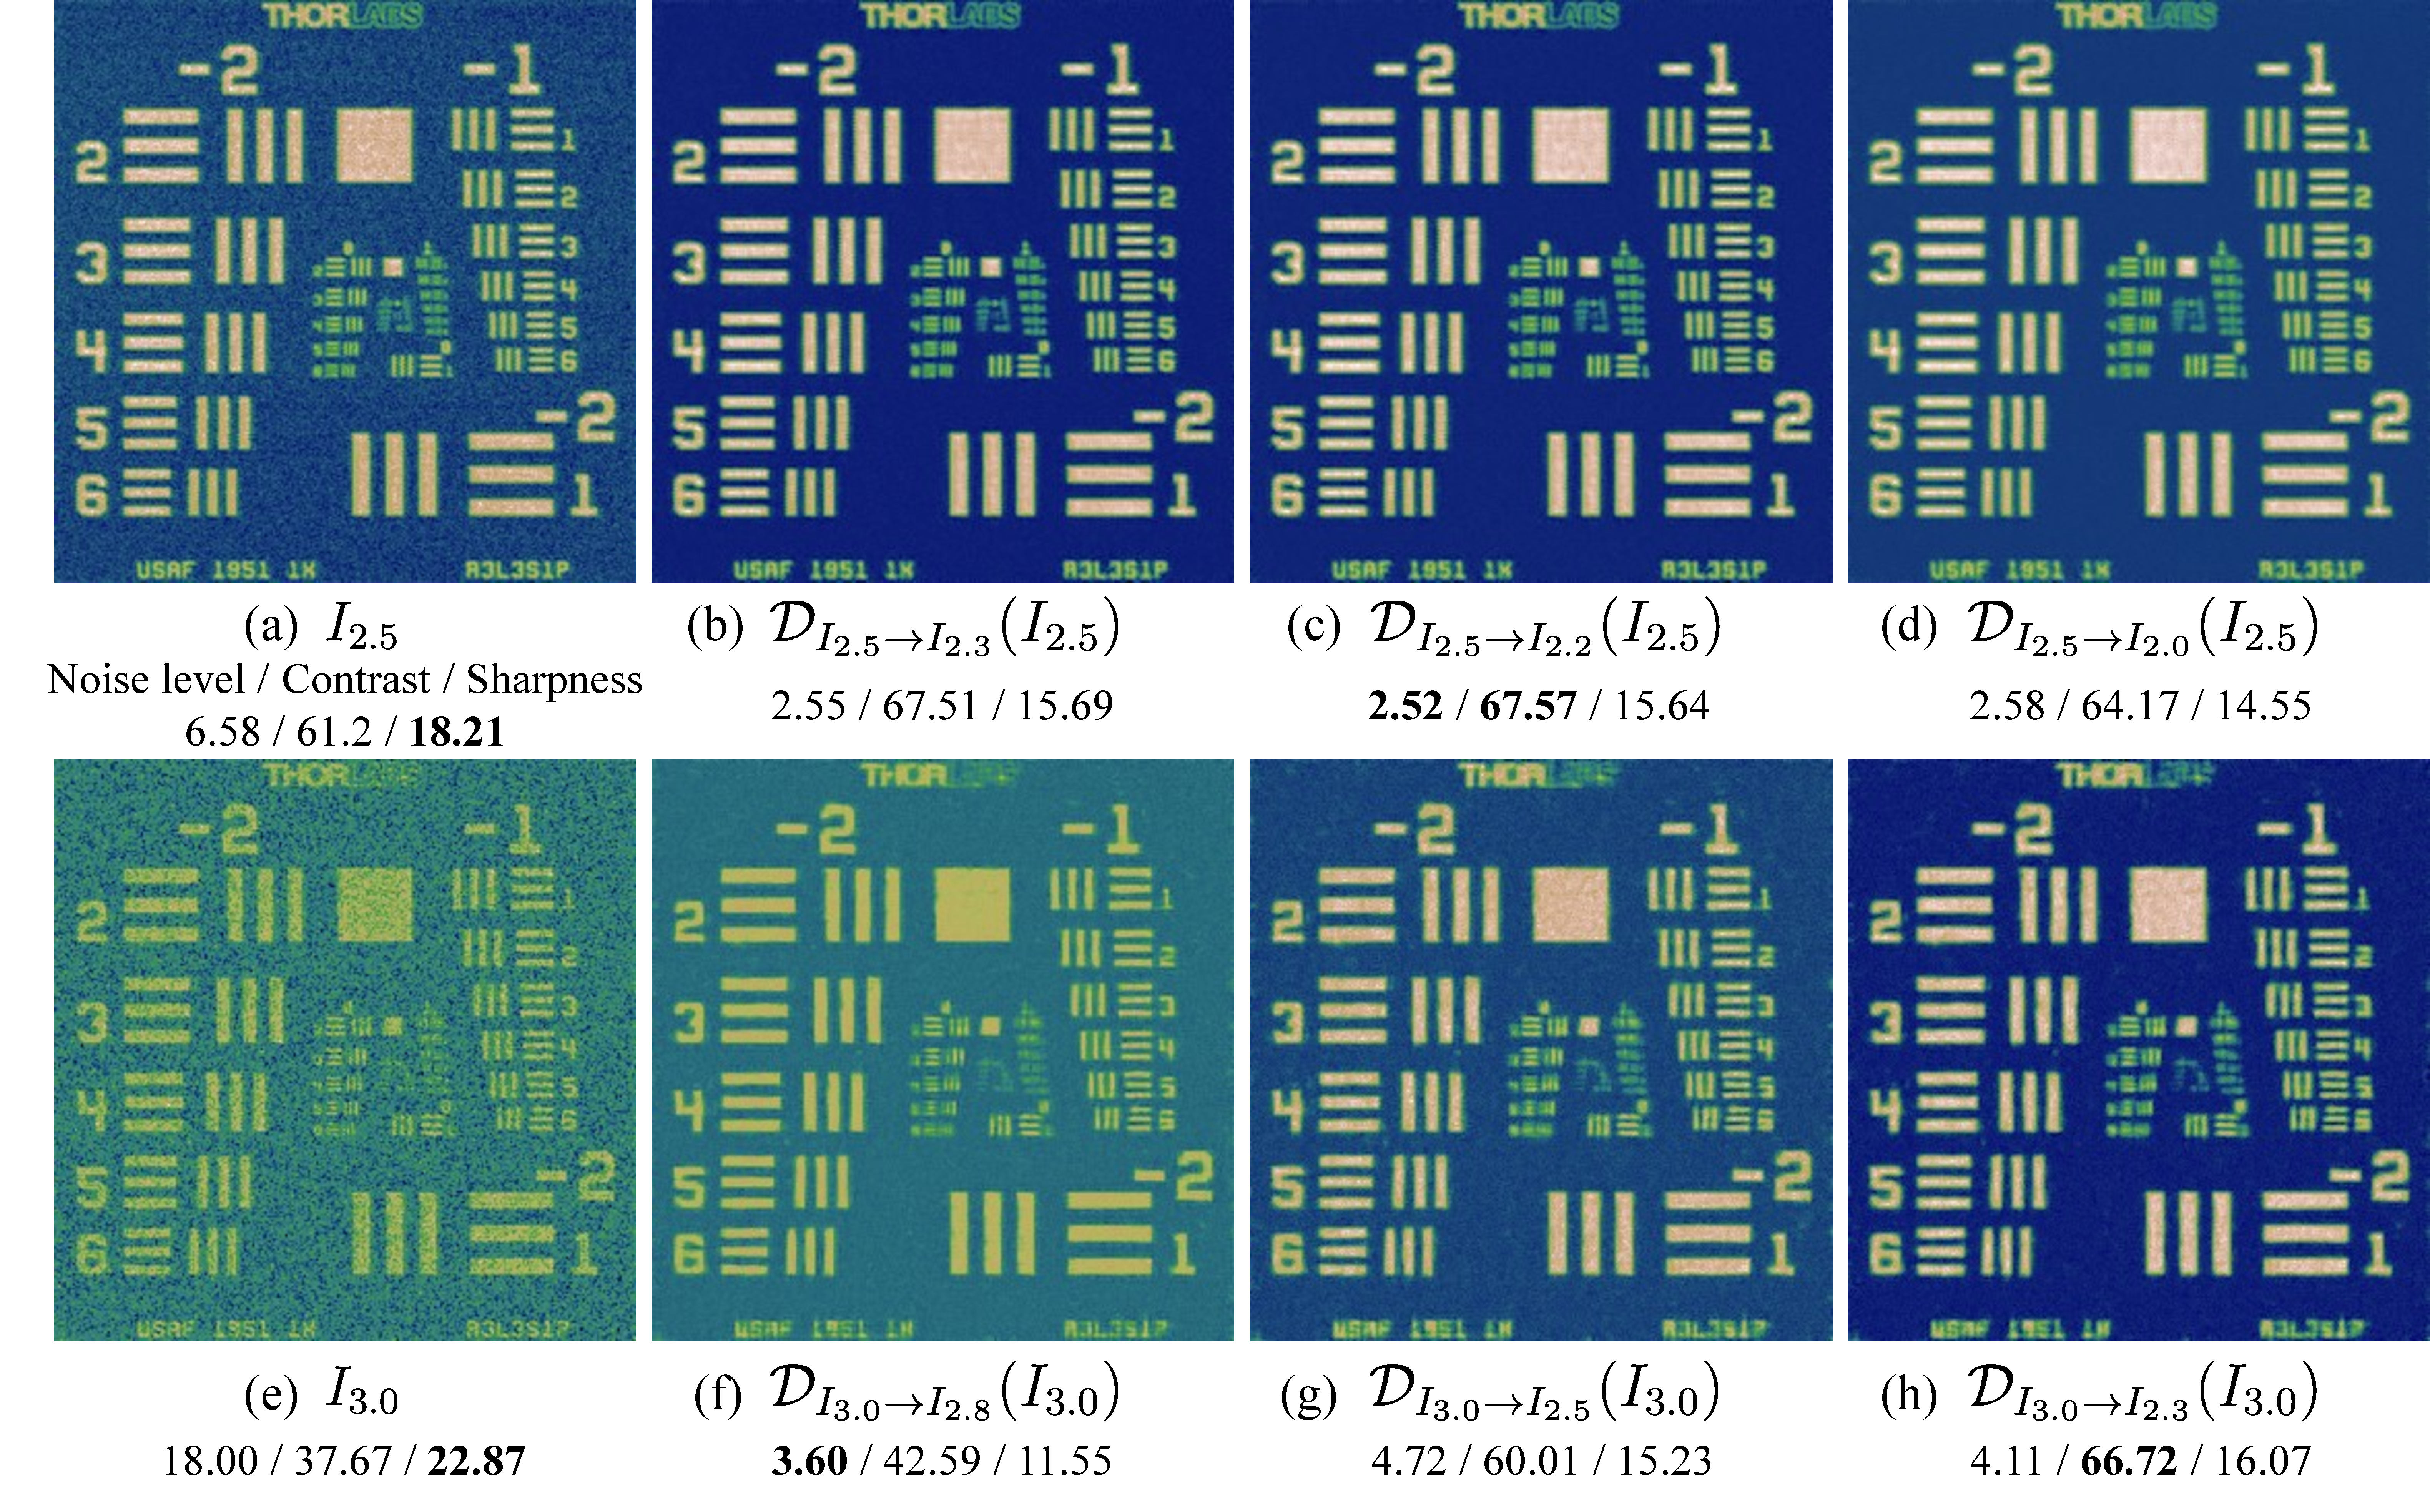
\includegraphics[width=\textwidth]{fig/Ryu-fig12.pdf}
    \caption{Self-supervised intra-data inference denoising results on 2.5 and 3.0 THz images based on O2O method. (a) Original 2.5 THz image; (b)-(d) O2O results of 2.5 THz image; (e) original 3.0 THz image; (f)-(h) O2O results of 3.0 THz image.}
    \label{fig:o2o_denoise}
\end{figure*}

In a THz-TDS system, as the frequency increases, the power of THz waves decreases, thus resulting in increased image noise levels. In this case, by emulating noise-free images at lower frequencies, effective noise reduction can be achieved in high-frequency images with slight loss in sharpness. This corresponds to the case involving the proposed O2O method with $\alpha > \beta$. This approach is key for improving image quality in the THz domain and can solve the issue of image noise at high frequencies.
Fig.~\ref{fig:o2o_denoise} shows the visual results of denoising high-frequency images at 2.5 and 3.0 THz. The first column shows the original images before model inference, and the remaining columns represent the results of noise reduction using models trained by fixing the source-image frequency $\alpha$ and adjusting the target-image frequency $\beta$. The noise levels and contrast values are indicated below each image. In all results, both the visual and quantitative noise levels decreased compared with the result of original images. The contrast improved as the noise decreased. The degree of noise reduction and contrast enhancement varied depending on the $\beta$ value. In the 2.5 THz image, the noise level decreased by approximately 62\% compared with the original, whereas in the 3.0 THz image, it decreased by 74\%-80\% as shown in Figs.~\ref{fig:o2o_denoise}b-\ref{fig:o2o_denoise}d and \ref{fig:o2o_denoise}f-\ref{fig:o2o_denoise}h. However, since the images were trained to target lower frequency images, the sharpness decreased by 14\%-20\% and 30\%-49\% for the 2.5 and 3.0 THz images, respectively, after noise reduction. These results imply that to reduce noise in high-frequency images, which are sharp but noisy, some loss of sharpness should be tolerated.

Cross-data inference has also been applied to the denoising methods using THz SAHS images. Fig.~\ref{fig:o2o_denoise_cross} shows the results of applying cross-data inference to reduce noise in high-frequency images of the metal bookmark with the Korean Goryeo celadon shape. In all the inference results, the noise level decreased by 18\%-24\% and the contrast improved. In particular, more excellent noise reduction effects were observed at larger frequency spans. These results indicate that noise can be effectively reduced in the new THz images with entirely different shapes from the images used in training, thus proving that the proposed method can be universally applied to various types of images. This THz SAHS image-based denoising method decreases in sharpness only slightly owing to the use of low-frequency images. However, considering the high spatial resolution provided by high-frequency images, this learning method, which effectively removes image noise with a slight reduction in spatial resolution to achieve cleaner images can be useful in various fields. In fact, it is expected to be applicable to various imaging areas beyond THz imaging.

\begin{figure*}[htbp]
    \centering
    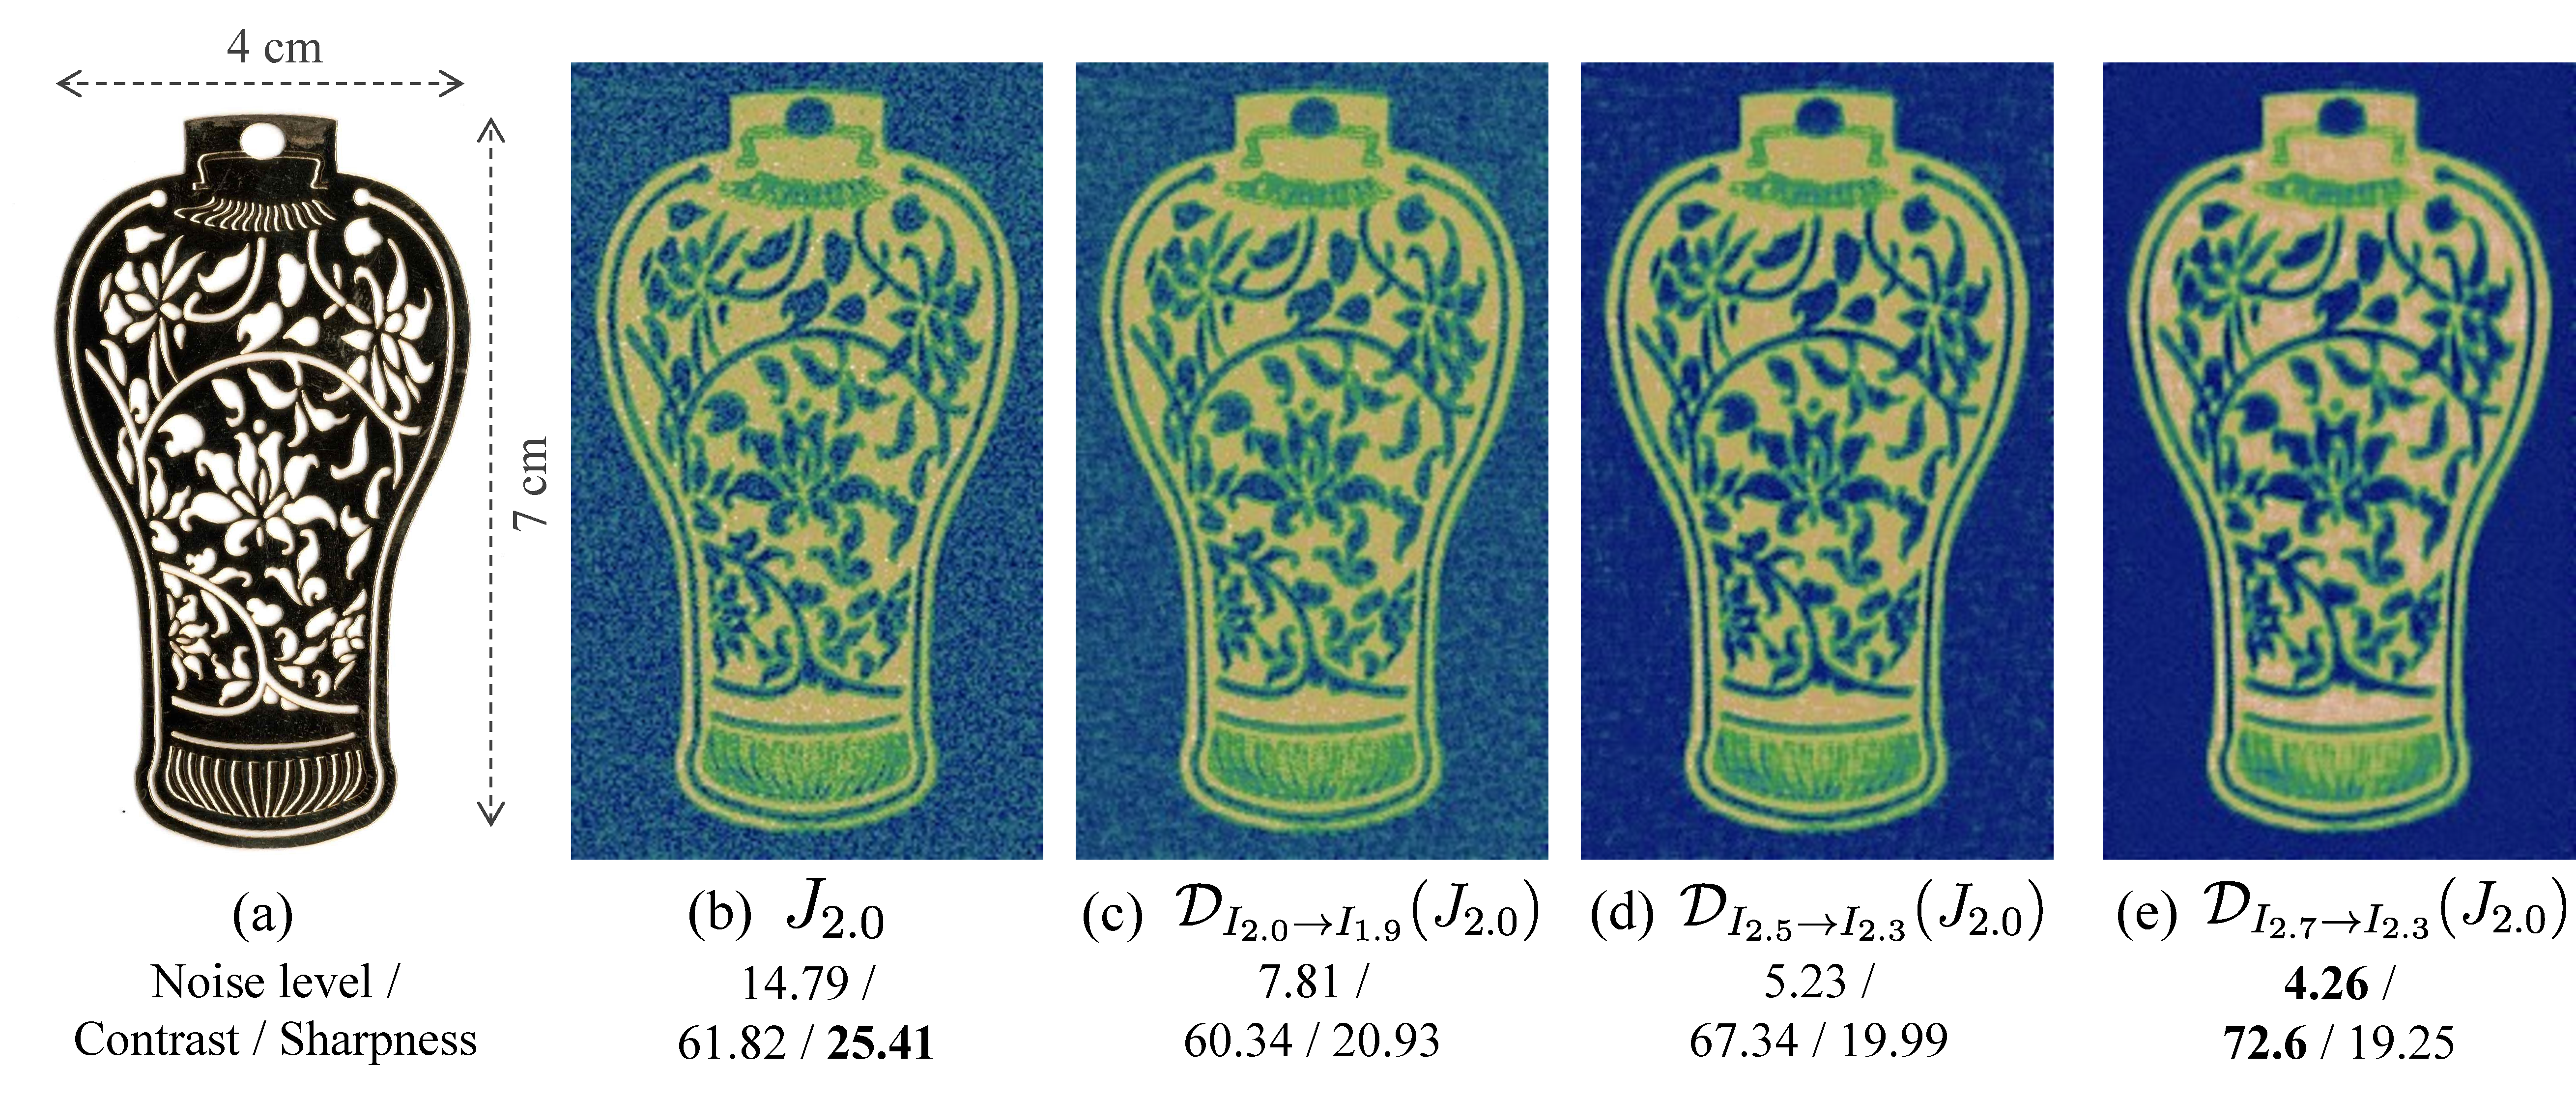
\includegraphics[width=\textwidth]{fig/Ryu-fig13.pdf}
    \caption{Self-supervised cross-data inference denoising results based on O2O method. (a) Metal bookmark optical image; (b) measured THz image of metal bookmark at 2.0 THz; (c)-(e) cross-data inference results using pretrained model $\mathcal{D}$.}
    \label{fig:o2o_denoise_cross}
\end{figure*}

\subsection{RE Results}
The effectiveness of the proposed RE method (Fig.~\ref{fig:recurrent_explain}) for further improving the O2O results described in Section~\ref{sec:intra} was evaluated. Fig.~\ref{fig:recurrent} shows the results of applying the RE method to 1.8 and 2.0 THz images. Figs.~\ref{fig:recurrent}b and f show the results of the O2O inference. And Figs.~\ref{fig:recurrent}c and g show the results of one recurrence, obtained from re-inferring the image using a model trained with the target as the source and the once-inferred result as the target in Figs.~\ref{fig:recurrent}b and f. Figs.~\ref{fig:recurrent}d and h show the results of the two recurrences. In the case of the 1.8 THz image, the sharpness and contrast increased with each recurrence, showing visually sharper and improved results. However, for the 2.0 THz image, the sharpness and contrast were at their best in the result of the first recurrence. Moreover, as the number of recurrences increased, the distinction between the index bars became clearer; however, the pixel values reduced significantly.
\begin{figure*}[htbp]
    \centering
    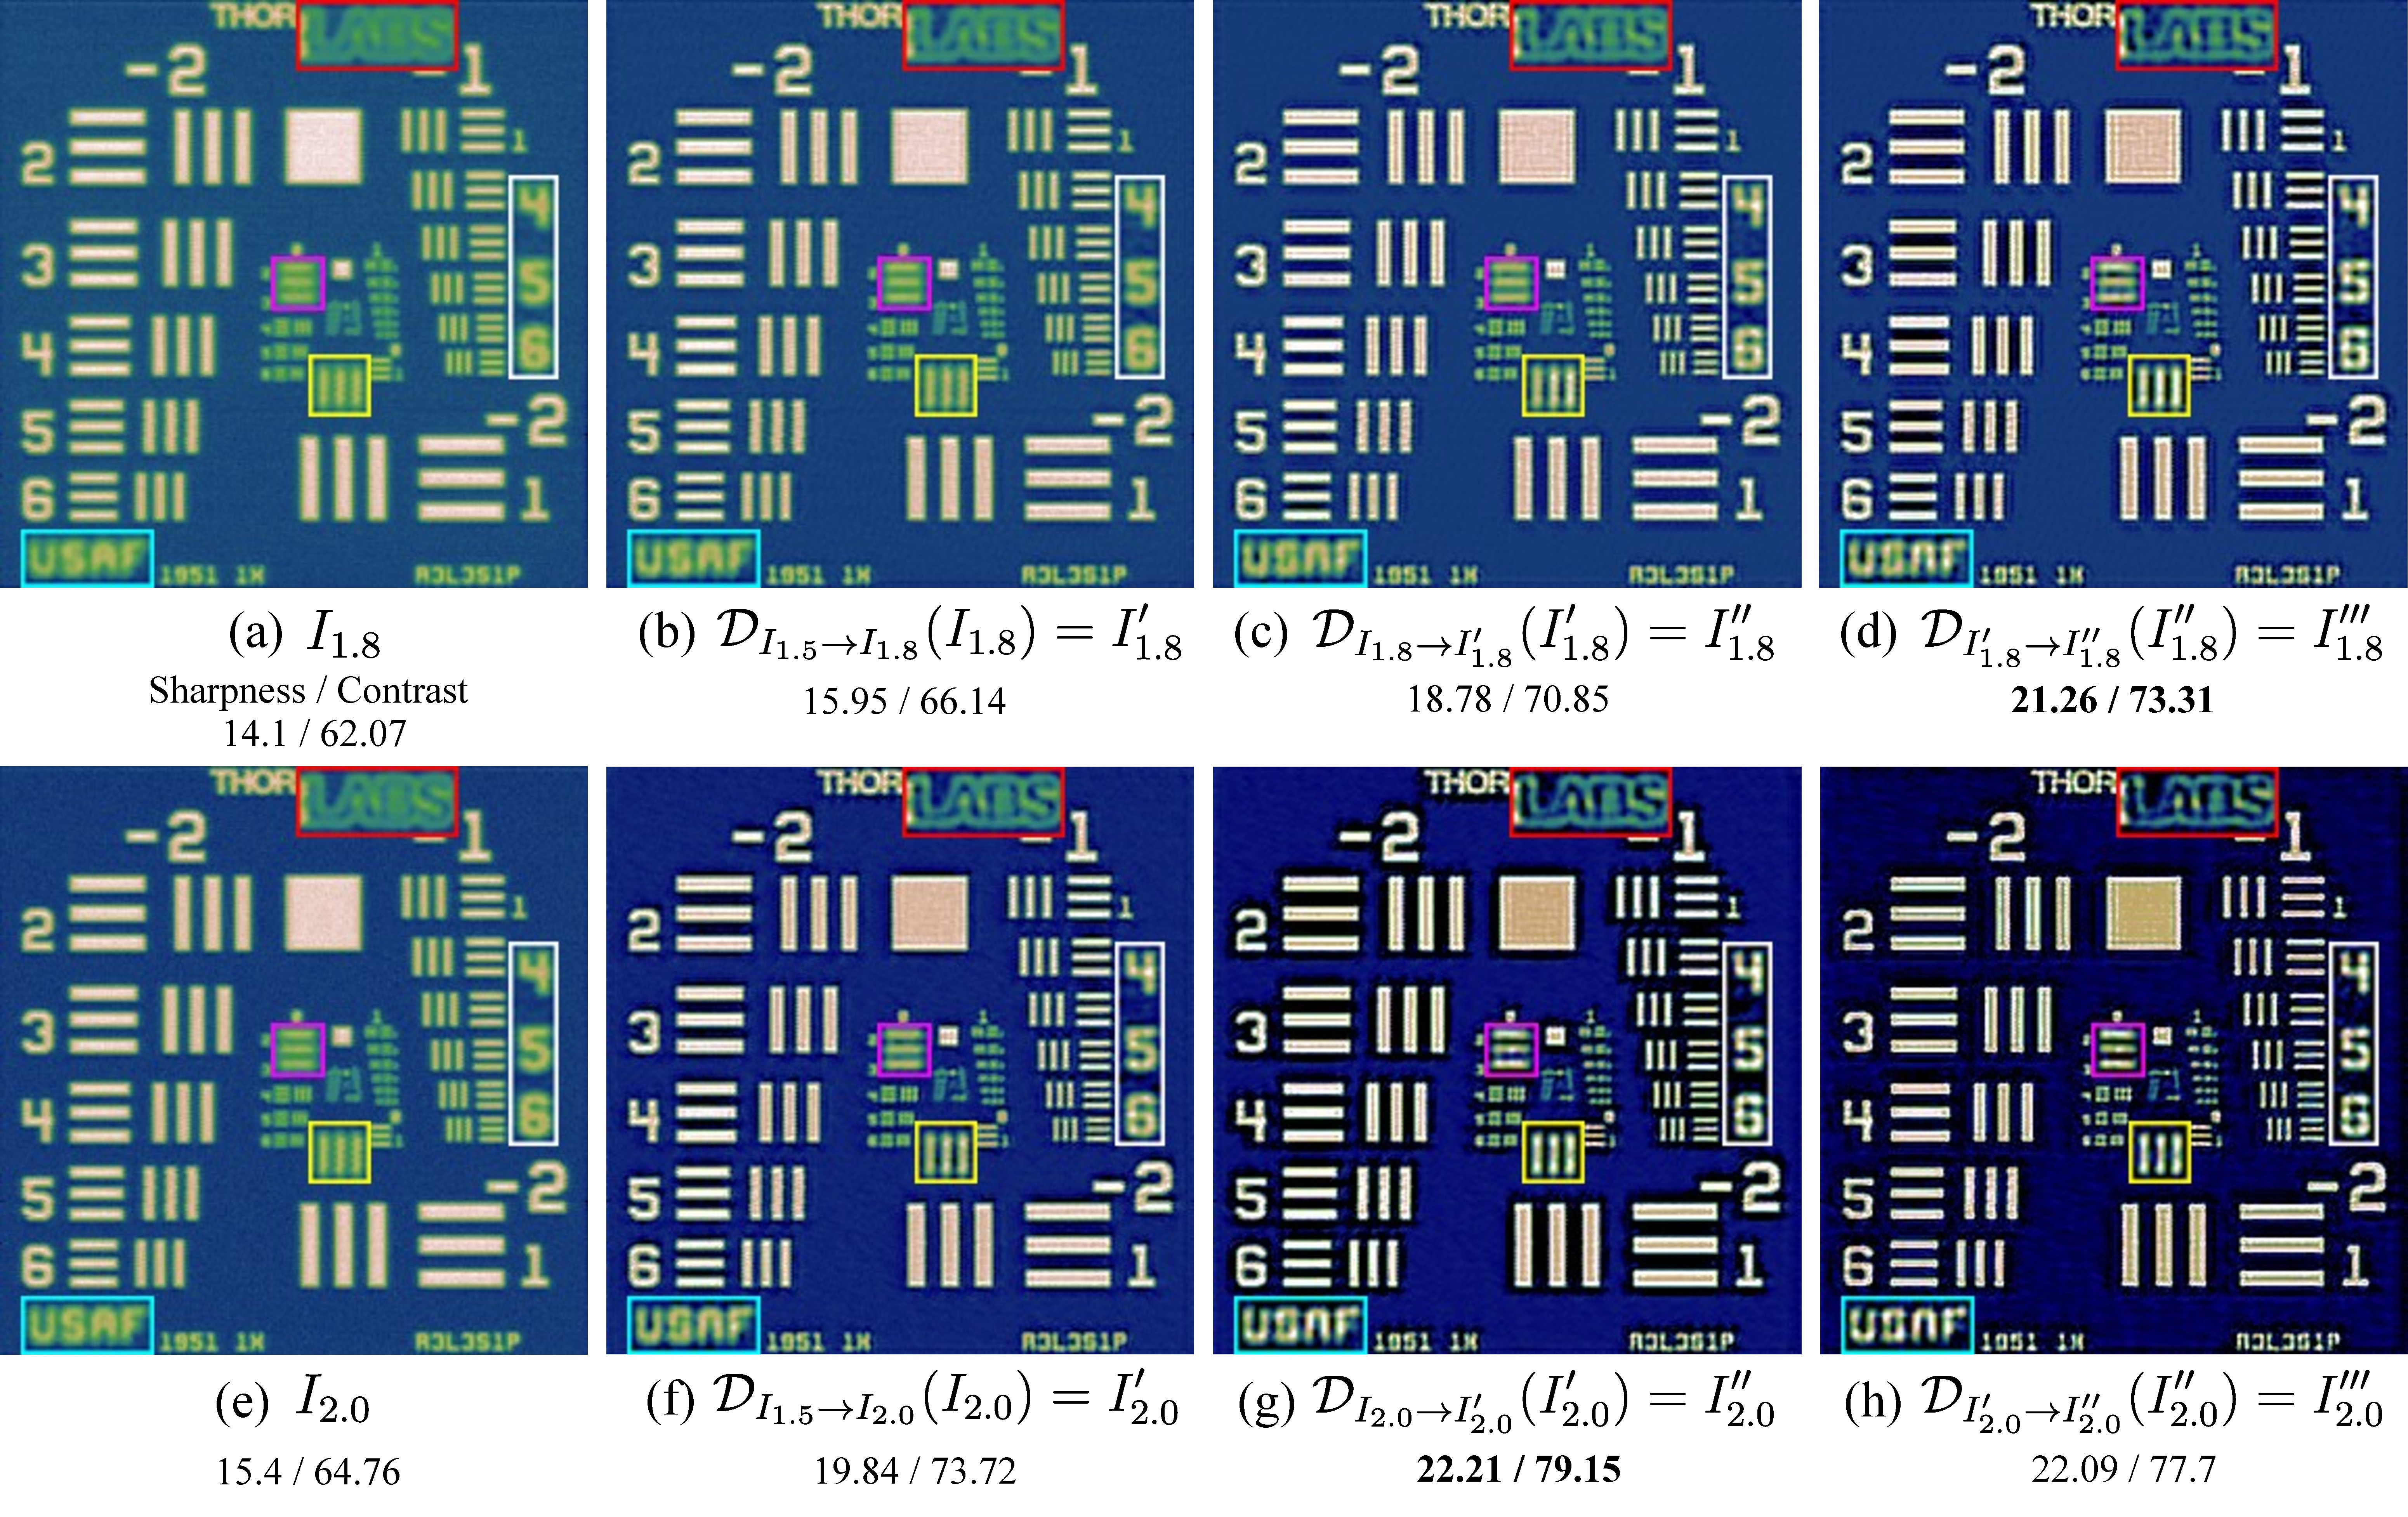
\includegraphics[width=\textwidth]{fig/Ryu-fig14.pdf}
    \caption{RE deblurring results based on 1.8 and 2.0 THz images.}
    \label{fig:recurrent}
\end{figure*}
To analyze the spatial resolution characteristics of the RE inference images shown in Fig.~\ref{fig:recurrent}, spatial-frequency spectrum analysis was conducted and the results are displayed in Fig.~\ref{fig:recurrent_spectrum}.
As the RE inference step advanced, the contrast of the boundaries intensified progressively, and the sharpness improved compared with that of the original image. The increase in contrast at key feature points, such as the central intersection, was more pronounced compared with that at the surrounding areas, thus reflecting sharper edges and a distinct contrast. This indicates that the RE inference process effectively amplifies the high-frequency components of the image, thereby effectively restoring the resolution and sharpness. Additionally, the ratio of the high-frequency energy was calculated and is indicated below each image. This ratio, which represents the energy in the high-frequency region of the spatial-frequency spectrum image, excludes the central section, which represents the low-frequency components. Higher values indicate sharper images. The proportion of high-frequency components increased with the number of recurrences, thus quantitatively confirming that the images became sharper.

\begin{figure*}[htbp]
    \centering
    \includegraphics[width=0.95\textwidth]{fig/Ryu-fig15.pdf}
    \caption{Spatial frequency spectrum of RE deblurring results based on 1.8 and 2.0 THz images.}
    \label{fig:recurrent_spectrum}
\end{figure*}

To analyze the excessive reduction in pixel values between the index bars of the inference image as the RE counts increased, we compared the pixel values of the optical image of the index bars of the positive USAF 1951 resolution target with the pixel values of the results of THz image inference using RE learning (see Figs.~\ref{fig:axial} and~\ref{fig:axial2}).
Figs.~\ref{fig:axial}a and~\ref{fig:axial2}a show the optical images of the USAF target. The pixel values along the red lines in these images were analyzed to evaluate the performance of the models inferred through RE learning. In Figs.~\ref{fig:axial}b and c and Figs.~\ref{fig:axial2}b and c, the cross-sectional pixel values of the optical images are presented alongside the RE inference results of the 1.8 and 2.0 THz images for comparison. The dashed black line represents the optical image, the dotted red line represents the original THz image, and the green line represents the image inferred by the O2O learning model. Additionally, the blue and purple lines represent the results of inferences made after applying RE once and twice, respectively.

Images inferred using the THz SAHS image-based model showed clearer distinctions between lines compared with the original THz images. This was particularly evident when RE model was used, which rendered the distinction between the lines as close as possible to the optical image. However, as the application of the RE model increases, although the distinction between lines becomes clearer, a dip appears at the center of the lines, thus resulting in image distortion. Therefore, the number of applications of the RE method in THz image processing should be determined meticulously based on the purpose of image acquisition.

Table~\ref{tab:beam_width} lists the beam widths calculated from Fig.~\ref{fig:axial2}(a) as full width at half maximum (FWHM) values. As shown, the beam width decreased as the operating frequency and the number of repetitions of the RE model increased. The beam widths for the 1.8 and 2.0 THz images were 0.776 mm and 0.721 mm, respectively. The beam width of the 1.8 THz image was reduced to 0.651 mm after one inference, which is a lower value than the beam width of the 2.0 THz image. The results quantitatively prove that the RE method can surpass the diffraction limit of THz images.

\begin{figure*}[htbp]
    \centering
    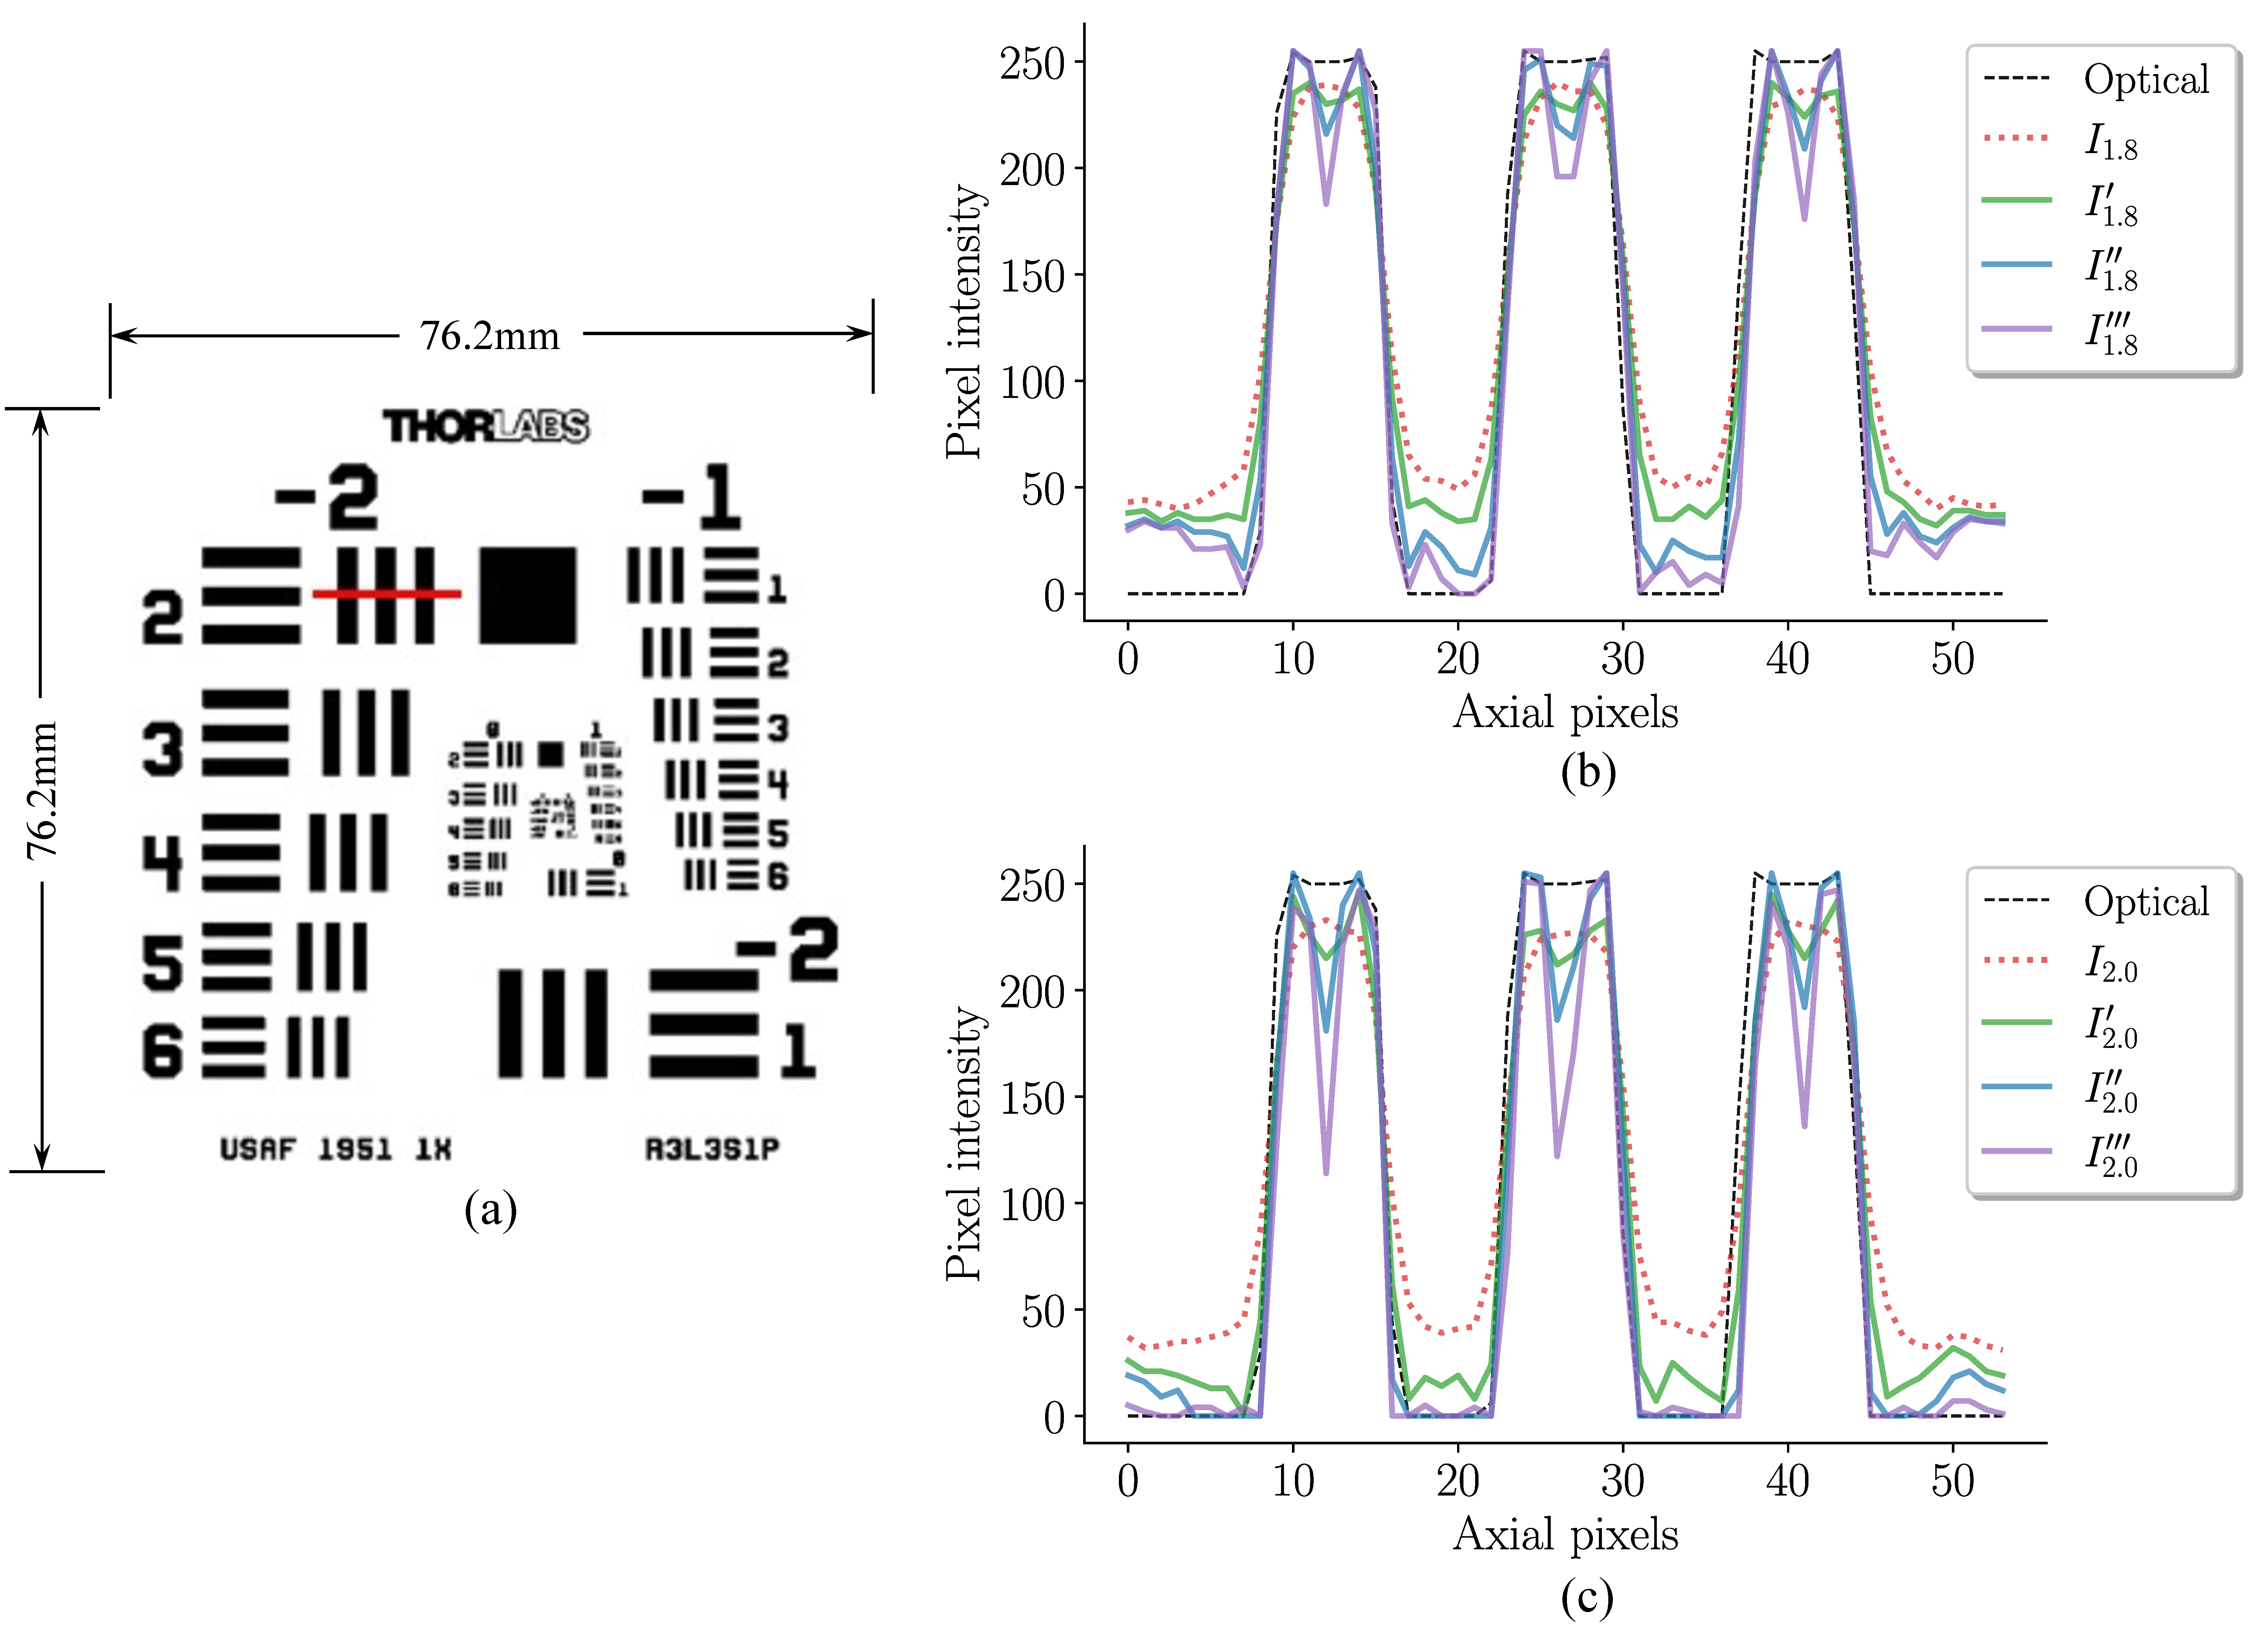
\includegraphics[width=0.7\textwidth]{fig/Ryu-fig16.pdf}
    \caption{Axial line graph comparison of improved results for 1.8 and 2.0 THz images.}
    \label{fig:axial}
\end{figure*}

\begin{figure*}[htbp]
    \centering
    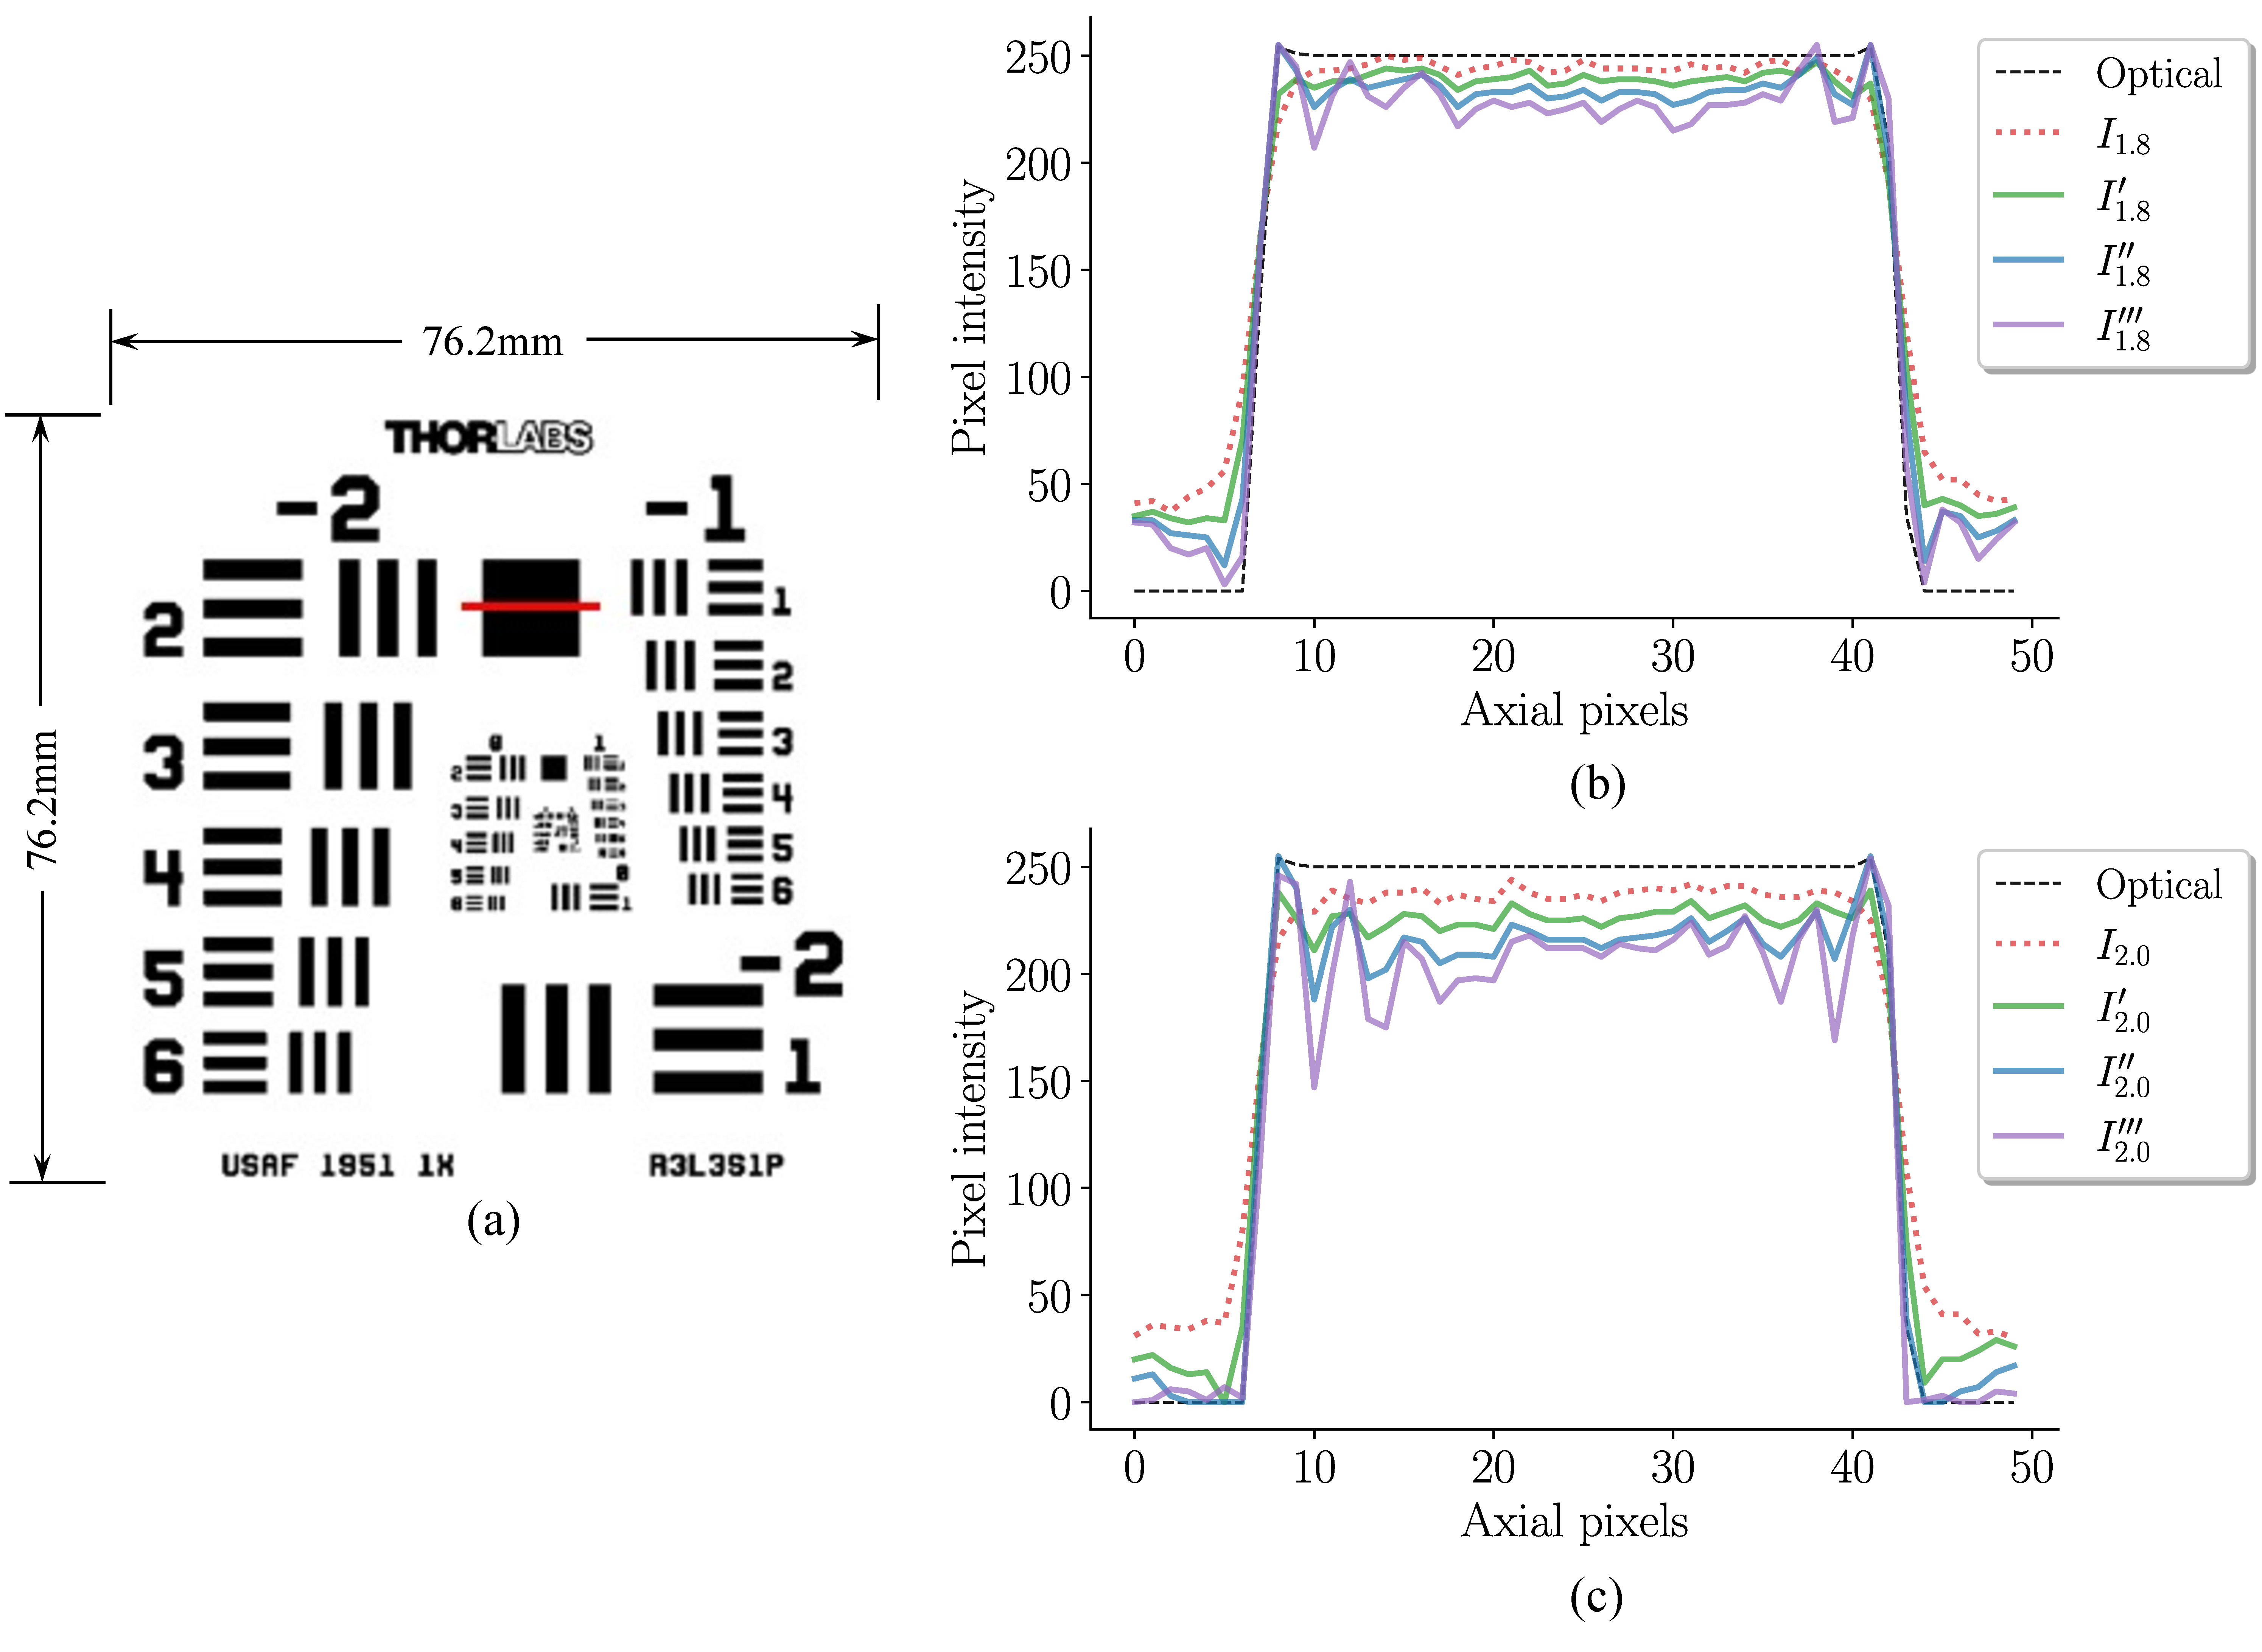
\includegraphics[width=0.7\textwidth]{fig/Ryu-fig17.pdf}
    \caption{Axial line graph comparison of improved results for 1.8 and 2.0 THz images.}
    \label{fig:axial2}
\end{figure*}


\begin{table}
    \centering
    \renewcommand{\arraystretch}{1.5} % Adjust the row height
    \begin{tabular}{c|c||c|c}
         \toprule
         \textbf{Image} & \textbf{Beam Width (mm)} & \textbf{Image} & \textbf{Beam Width (mm)} \\
         \midrule
         $I_{1.8}$ & 0.776 &$I_{2.0}$ & 0.721 \\
         $I_{1.8}'$ & 0.651 &$I_{2.0}'$ & 0.573 \\
         $I_{1.8}''$ & 0.566 &$I_{2.0}''$ & \textbf{0.506} \\
         $I_{1.8}'''$ & \textbf{0.530} &$I_{2.0}'''$ & \textbf{0.506} \\
         \bottomrule
    \end{tabular}
    \caption{Beam width measured as full width at half maximum (FWHM) of RE results.}
    \label{tab:beam_width}
\end{table}

\subsection{Image Super-Resolution}
Owing to the inherently low resolution of THz images, ZSSR was applied to enhance the resolution, as shown in Fig.~\ref{fig:zssr}. Fig.~\ref{fig:zssr}a displays the original 2.0 THz image, Fig.~\ref{fig:zssr}b shows the image with improved quality without scale change, and Fig.~\ref{fig:zssr}c presents the result with a scale factor of two, which resulted in a $584\times 584$ resolution image. The environment for training and inferring ZSSR is identical to that for the O2O learning. Even under the same O2O training, applying ZSSR with a scale factor of two resulted in a sharper image.
Fig.~\ref{fig:zssr_spectrum} illustrates the spatial frequency spectrum and high-frequency energy ratio for the images shown in Fig.~\ref{fig:zssr}. As the process progresses from the original image to the O2O inferred image and the 2x-expanded ZSSR inferred image, the textures and edges became clearer and high-frequency components became more conspicuous. The enlargement of the image scale further highlighted these features. In particular, the high-frequency energy ratio in the original 2.0 THz image increased from 0.1039 to 0.2114 after applying ZSSR, thus providing quantitative evidence of resolution improvement. These results prove that applying ZSSR to SAHS images acquired using a THz-TDS system can significantly improves the image quality compared with the original image.

\begin{figure*}[htbp]
    \centering
    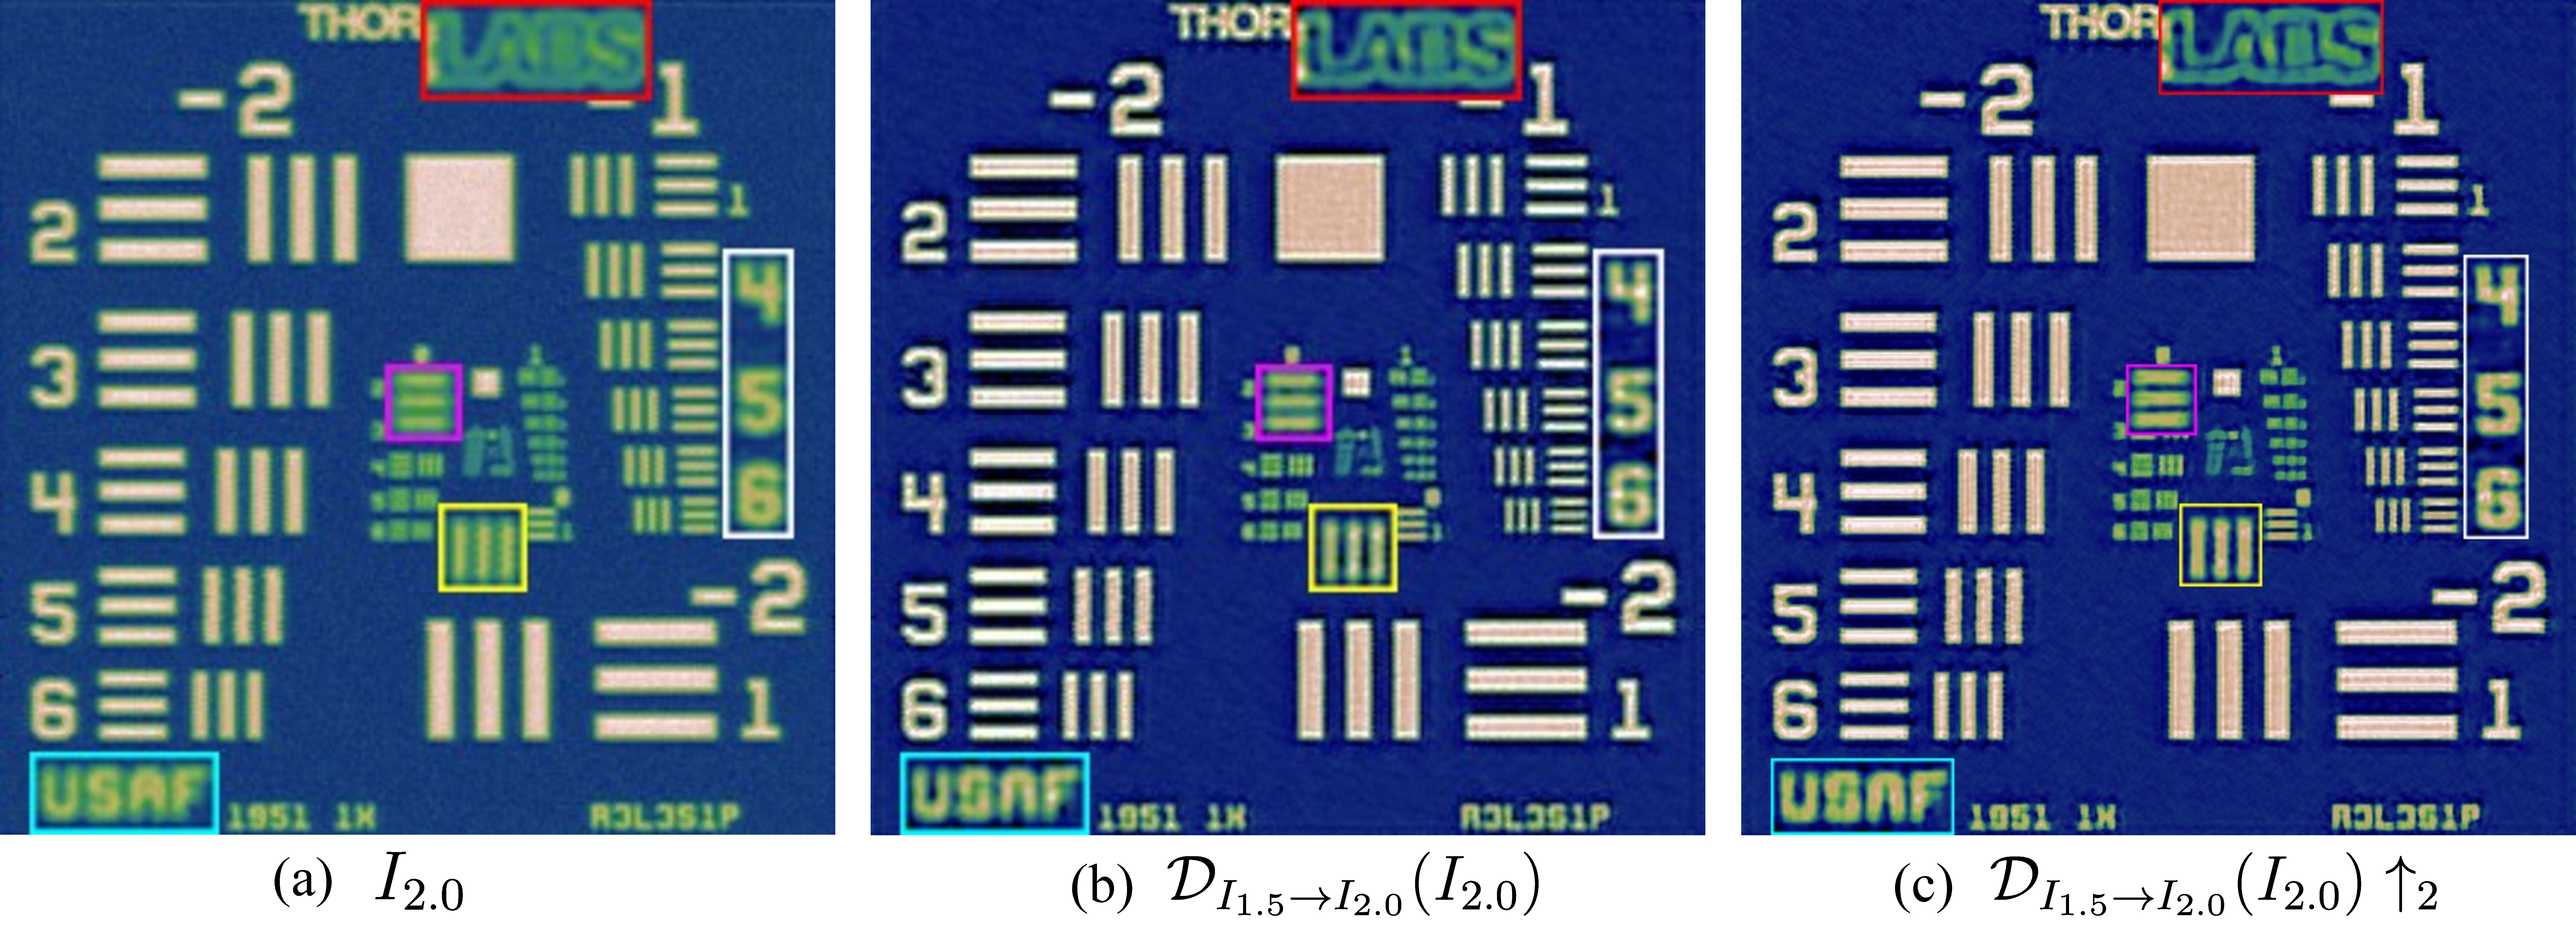
\includegraphics[width=\textwidth]{fig/Ryu-fig18.pdf}
    \caption{ZSSR results after applying O2O method. (a) Original 2.0 THz image; (b) O2O result ($\alpha=1.5,\beta=2.0,\gamma=2.0$); (c) ZSSR result of (b).}
    \label{fig:zssr}
\end{figure*}

\begin{figure*}[htbp]
    \centering
    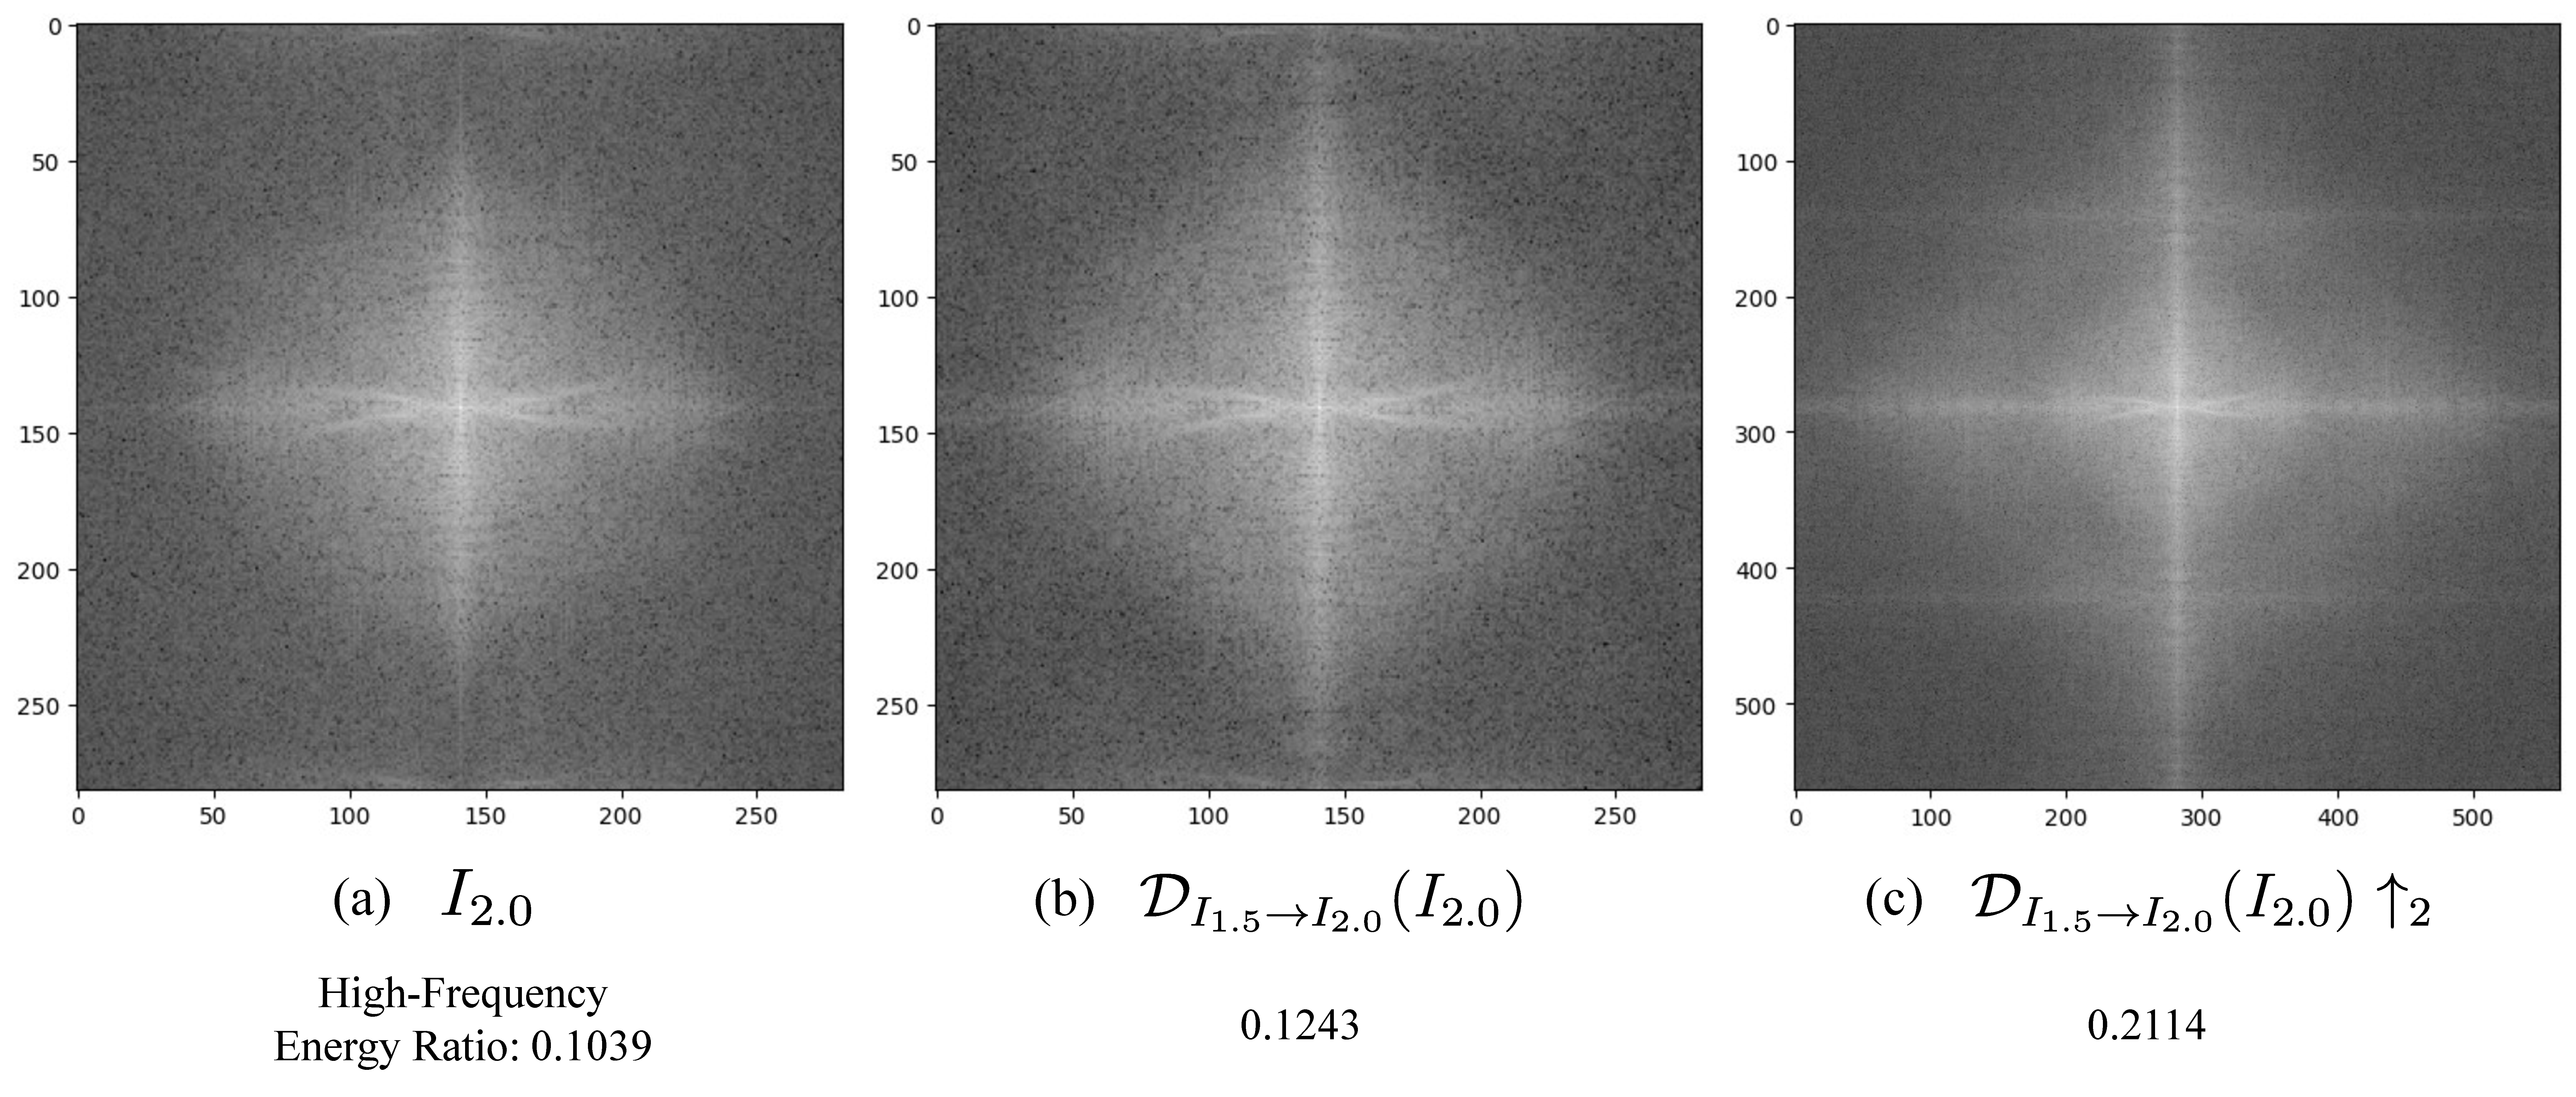
\includegraphics[width=0.95\textwidth]{fig/Ryu-fig19.pdf}
    \caption{Spatial frequency spectrum of ZSSR results.}
    \label{fig:zssr_spectrum}
\end{figure*}


%%% ---------- Subsection: Model Comparison ---------- %%%
\subsection{Model Comparison}
To demonstrate the efficacy of the proposed THz image-restoration method, we compared it with other deep learning-based image restoration methods, as shown in Fig.~\ref{fig:model-comp}. For a unbiased comparison, we applied a 2x resolution-enhancement process to all the other image-restoration methods, similar to our proposed learning method. The original 2.0 THz image has 282$\times$282 pixels, while the other results all have a resolution doubled to 584$\times$584 pixels. Consequently, except for the original image, all inferred images indicated a 2x increase in resolution, which resulted in a relative decrease in sharpness compared with the original image owing to the increased total number of pixels. Therefore, when evaluating the sharpness performance of the inferred images, one should compare the sharpness of the images excluding that of the original image.
Fig.~\ref{fig:model-comp}a shows the original 2.0 THz image. Figs.~\ref{fig:model-comp}b, c, and d show the images with twice the resolutions in the horizontal and vertical directions, which were achieved using networks proposed by Long et al.~\cite{longTerahertzImageSuperresolution2019}, HAN~\cite{niu2020han}, and NAFNetSR~\cite{chu2022nafssr}, respectively. Long et al.~\cite{longTerahertzImageSuperresolution2019} adopted a residual learning network structure, trained using a random degradation model. Figs.~\ref{fig:model-comp}c and d for HAN and NAFNetSR, represent state-of-the-art models in image SR. which were trained using the DIV2K dataset and degraded randomly using blur kernel widths measuring between 0.1 and 3~\cite{longTerahertzImageSuperresolution2019}.
Fig.~\ref{fig:model-comp}e shows the result of blur removal using pretrained NAFNet~\cite{chen2022simple} weights and by applying ZSSR. Fig.~\ref{fig:model-comp}f shows the results of training and inference using a combination of self-supervised learning on THz SAHS images and ZSSR, as proposed in this study. The ZSSR-applied images presented in Figs.~\ref{fig:model-comp}e and f appeared sharper and performed better numerically. In particular, in the yellow box, the edges became sharper and the boundaries were more clearly distinguished. In Figs.~\ref{fig:model-comp}b-\ref{fig:model-comp}d, where artificial Gaussian blur was applied and then restored, the edges became rounded and were smudged. This is because the artificial degradation implemented during the training was not optimized for the characteristics of the actual THz images. Based on Fig.~\ref{fig:model-comp}e, distortion in the form of a new blurred pattern in the background occurred owing to the addition of ZSSR after NAFNet, thus indicating that NAFNet and ZSSR did not integrate organically. As shown in Fig.~\ref{fig:model-comp}f, our proposed method yielded the highest sharpness and contrast, both visually and numerically. This is because our proposed method applies an image restoration method using pure frequency characteristics without artificial manipulation, utilizes THz SAHS images for self-supervised learning, and effectively combines image restoration with SR by integrating ZSSR into the self-supervised learning process.

\begin{figure*}[htbp]
    \centering
    \includegraphics[width=0.9\textwidth]{fig/Ryu-fig20.pdf}
    \caption{Performance comparison of deep THz image restoration methods. (a) Original 2.0 THz image; (b) results of Long et al.~\cite{longTerahertzImageSuperresolution2019}; (c) HAN~\cite{niu2020han}; (d) NAFNetSR~\cite{chu2022nafssr}; (e) NAFNet~\cite{chen2022simple}+ZSSR; (f) our results.}
    \label{fig:model-comp}
\end{figure*}
\section{Conclusion}
In this study, we proposed a deep learning-based self-supervised learning restoration method that leverages SAHS images acquired via a THz-TDS system to improve image quality. This innovative learning approach does not require additional training datasets or artificial image degradation; instead, it directly utilizes the frequency characteristics of THz SAHS images. Low-frequency images, which are constrained by the diffraction limits of their frequencies, typically cannot achieve the sharpness of high-frequency images. However, our method successfully emulates high-frequency images, thereby overcoming the diffraction limits. Additionally, in typical THz systems, the SNR decreases with increasing frequency, thus resulting in noisy images at higher frequencies despite their enhanced sharpness. To address this issue, we used THz SAHS images to train models that learned low-noise images at lower frequencies, thus effectively reducing noise in high-frequency images.

Additionally, we introduce three frameworks based on self-supervised learning using THz SAHS images. First, we propose an O2O-mapping learning method to learn the mapping between two frequencies. This method enhances the sharpness of low-frequency images beyond their diffraction limits and reduces noise in high-frequency areas with a low SNR. The frequency relationship between the source, target, and inference images critically affects the inference performance. Thus, the source and target frequencies as well as the frequency of the inference image frequency must be selected appropriately to optimize the image quality. Furthermore, we demonstrated quality improvements in new THz images not used during training, which signified the broad applicability and potential of the proposed method in various THz imaging systems. Second, we propose an RE learning method that recurrently applies O2O learning to further improve the image quality. As the number of RE iterations increased, the distinctness between the index bars of the target objects in the test images became more pronounced. However, excessive iterations can lead to image distortion, thus highlighting the importance of judiciously determining the number of RE learning applications required for optimal image quality. Finally, we integrated ZSSR into our learning process to enhance image resolution. This method utilizes purely natural frequency relationships in THz SAHS images to achieve SR while overcoming diffraction limits. Integrating ZSSR into the proposed self-supervised learning process significantly enhanced image quality compared with other state-of-the-art image restoration methods.

The main contribution of this study is the proposal of a novel framework for improving image quality based on self-supervised learning using THz SAHS images. This methodology has proven to be effective in significantly enhancing the sharpness of THz images in the low-frequency domain and reducing noise in the high-frequency domain. Our method is applicable to both trained and new images, thus indicating its potential for application in various THz imaging systems. Additionally, by leveraging pure frequency relationships, our proposed learning approach is expected to improve image quality when applied across a wide range of imaging systems.

\section*{Acknowledgements}
This work was supported by the Basic Science Research Program through the National Research Foundation (NRF) funded by the Ministry of Science and ICT (grant no. NRF-2021R1F1A1059493) and Institute of Information \& Communications Technology Planning \& Evaluation (IITP) grant, funded by the Korea government (MSIT) (Grant No. 2022-0-01044, Development of terahertz wave-based real-time intelligent brain tumor diagnosis system and technology).

\bibliographystyle{IEEEtran}
\bibliography{egbib}

% ========== Biography ============ %
\vspace{-10mm}
\begin{IEEEbiography}[{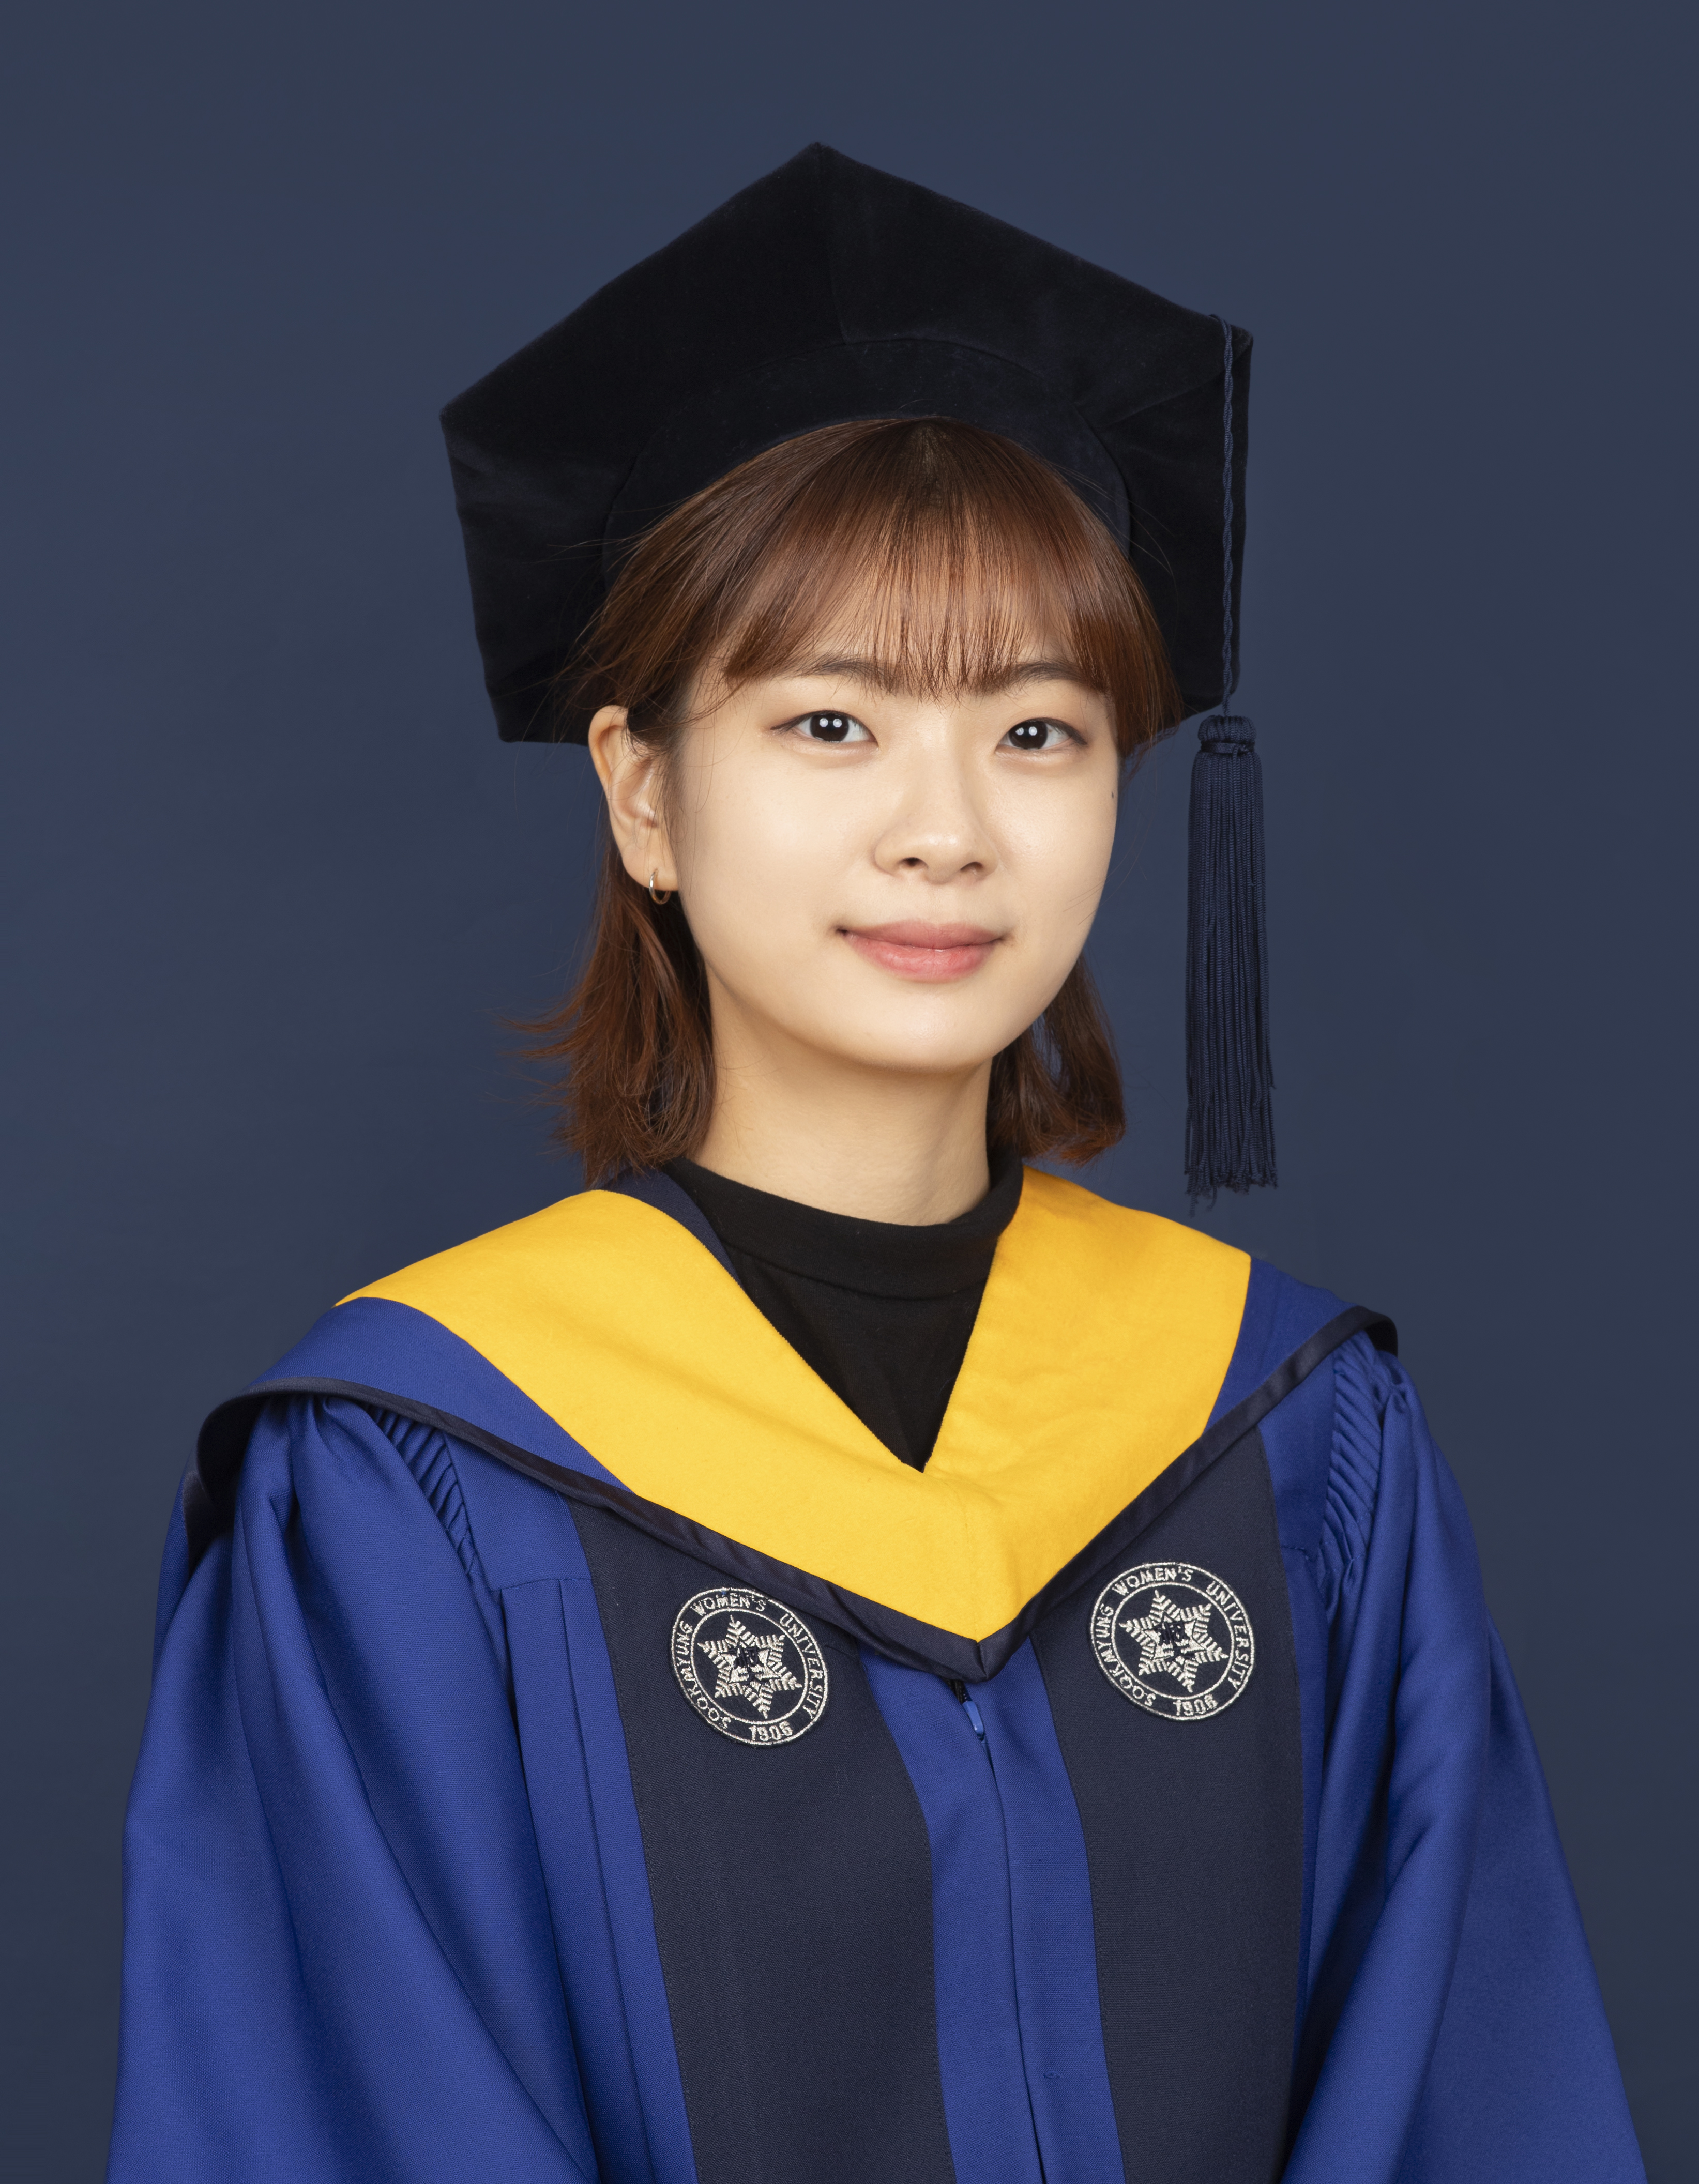
\includegraphics[width=1in,height=1.25in,clip,keepaspectratio]{biography/yeo}}]{Woon-Ha Yeo}
received her B.Eng. and M.Eng. in IT Engineering from Sookmyung Women's University, South Korea, in 2019 and 2021. She is currently a Ph.D. student at Sahmyook University and a researcher affiliated to TAIIPA, South Korea. Her research interests include deep learning, computer vision and terahertz image processing.
\end{IEEEbiography}
\vspace{-10mm}
\begin{IEEEbiography}[{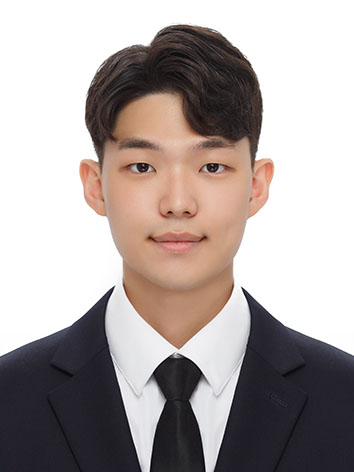
\includegraphics[width=1in,height=1.25in,clip,keepaspectratio]{biography/jung}}]{Seung-Hwan Jung}
received his B.Eng. in IT Convergence Engineering from Sahmyook University, South Korea, in 2023. He is currently a Ph.D. student at Sahmyook University and researcher affiliated to TAIIPA, South Korea, His research interests include deep learning, computer vision and terahertz signal and image denoising.
\end{IEEEbiography}
\vspace{-10mm}
\begin{IEEEbiography}[{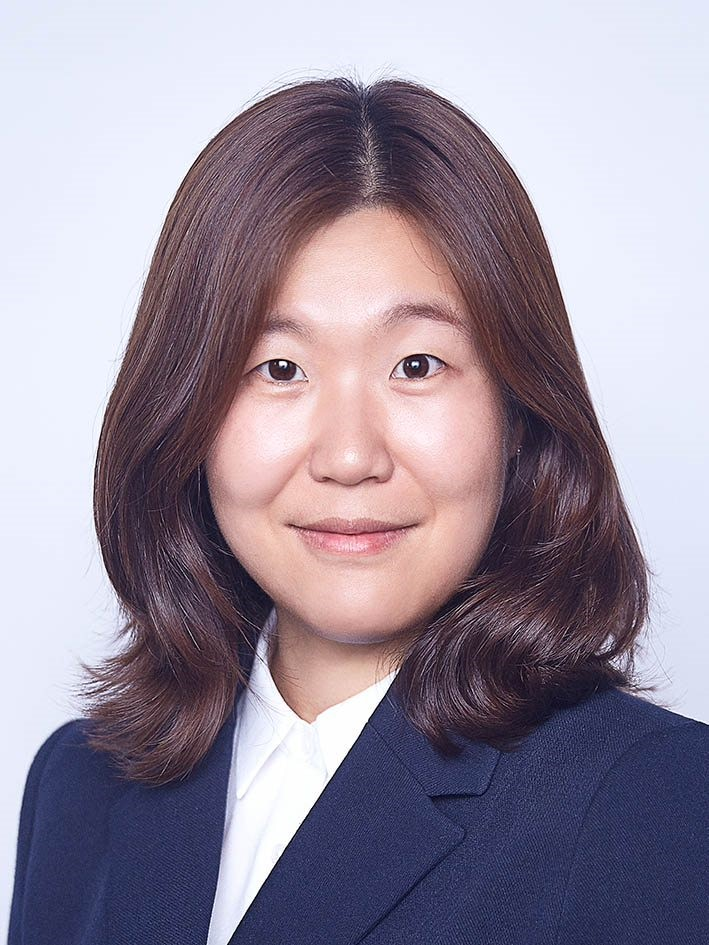
\includegraphics[width=1in,height=1.25in,clip,keepaspectratio]{biography/maeng}}]{Inhee Maeng}
is currently a research assistant professor at the YUHS-KRIBB, Medical Convergence Research Institute, Yonsei University. She received her Ph.D. from the Department of Physics at University of Seoul under the supervision of Professor Joo-Huik Son in 2012. Her research interests focus on the design and construction of various terahertz systems and their applications using emerging materials. In particular, she focuses on organic–inorganic hybrid perovskite materials for THz sensors.
\end{IEEEbiography}
\vspace{-10mm}
\begin{IEEEbiography}[{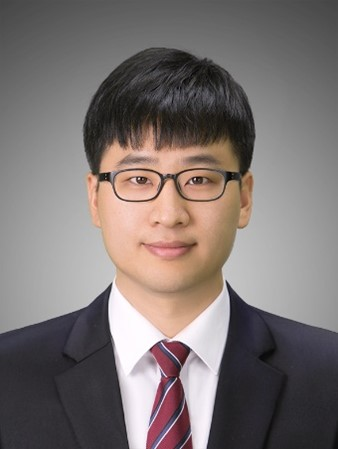
\includegraphics[width=1in,height=1.25in,clip,keepaspectratio]{biography/ji}}]{Youngbin Ji}
(Member, IEEE) was born in Busan, Republic of Korea, in 1980. He received the B.S. degree, M.S. degree and Ph.D. degree in electrical and electronic engineering from the Korea Maritime University, Busan, Republic of Korea, in 2006, 2008, and 2013, respectively. From 2013 to 2015, a Postdoctoral Fellow at the Yonsei University, Seoul, Republic of Korea. From 2015 to 2017, he was a Research assistant professor at the Yonsei University College of Medicine, Seoul, Republic of Korea. From 2017 to 2023, he was a senior researcher at the Gimhae Biomedical Industry Promotion Agency, Gyeongsangnam-do, Republic of Korea. He is currently a research associate professor at the Gwangju Institute of Science and Technology, Gwangju, Republic of Korea. His research has been concerned with medical and industrial application research using terahertz waves.
\end{IEEEbiography}
\vspace{-10mm}
\begin{IEEEbiography}[{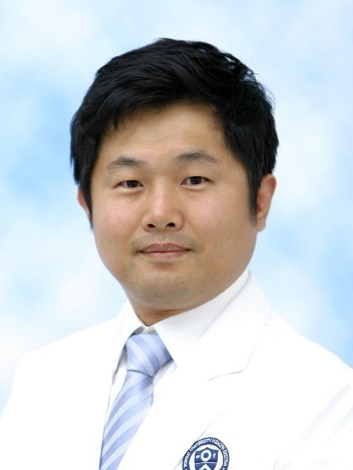
\includegraphics[width=1in,height=1.25in,clip,keepaspectratio]{biography/oh}}]{Seung Jae Oh}
received his B.S., M.S. and Ph.D. degrees in physics from the University of Seoul in 2000, 2002 and 2007, respectively. He was a post-doctoral research fellow at College of Medicine, Yonsei Univertisy since 2007 to 2009. In 2009, he was a research fellow at Department of Radiology, Yonsei University. He has been with YUHS-KRIBB Medical Convergence Research Institute, Yonsei University as a research assistant professor from 2010 to 2020 and research associate professor since 2020. His research interest is in the area of biomedical optics imaging that includes terahertz wave imaging and ultrafast laser biomedical application.
\end{IEEEbiography}
\vspace{-10mm}
\begin{IEEEbiography}[{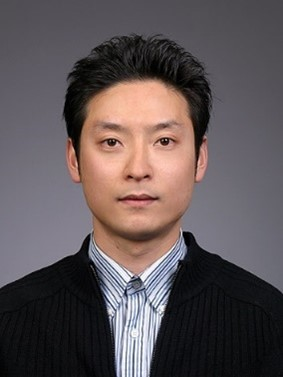
\includegraphics[width=1in,height=1.25in,clip,keepaspectratio]{biography/ryu}}]{Han-Cheol Ryu}
received a Ph.D. in electronic engineering from KAIST (Korea Advanced Institute of Science and Technology), Korea 2011. From 2002 to 2013, he worked as a senior researcher at ETRI (Electronics and Telecommunications Research Institute) in Korea. Since 2013, he has been a professor at Sahmyook University in Seoul, Korea. His research interests include artificial intelligence (machine learning and deep learning), microwave and terahertz-wave technology, and their applications in wireless communications, sensing, and imaging systems. In particular, he is focusing on research that applies deep learning techniques to terahertz imaging technology.
\end{IEEEbiography}
\vfill

\end{document}